\documentclass{article}
\usepackage[utf8]{inputenc}
\usepackage{hyperref}
\usepackage{amsmath}
\usepackage{amsfonts}
\usepackage{graphicx}
\usepackage{enumitem}
\usepackage{wrapfig}
\graphicspath{ {./images} }


\title{Freshman Physics}
\author{
    Tan Chien Hao\\
    \texttt{www.tchlabs.net}\\
    \texttt{Telegram @tch1001}
    % new collaborators add your name and contact here!
}

\date{\today}
\begin{document}
\newif\ifpaper

% TOGGLE ANSWER HERE
\papertrue

\maketitle

Updated notes are available at \url{https://bit.ly/physicsolympiadnotes}. Please inform me of any errors. Feel free to message me to explain something in greater detail :) I also run a weekly SJPO / SPhO class if you're interested.
\tableofcontents

\section{Math: Functions}
Lecture: \url{https://youtu.be/-Ia9Wv5USaE}\\[10pt]
Functions are maps from one set to another set. We denote them as $f: A \rightarrow B$ or $f(x) \in B$ where $x\in A$. \\
\\
Examples of functions $f: \mathbb R \to \mathbb R$:
\begin{itemize}
    \item Particle's x coordinate $x(t) = 5 \sin (2t)$
    \item Particle's x component of velocity $v_x(t) = 10 \cos (2t)$
    \item Particle's x component of acceleration $a_x(t) = - 20 \sin (2t)$
    \item Potential Energy of spring mass system $U(x) = \frac{1}{2} k(x-x_0)^2$
    \item Current flowing through Resistor Capacitor circuit $I(t) = I_0 e^{-{t}/{RC}}$
    \item Kinetic Energy in terms of speed $T(|\vec{v}|) = \frac{1}{2} m |\vec{v}|^2$
\end{itemize}
\leavevmode \\
Examples of functions $f: \mathbb R \to \mathbb R^3$:
\begin{itemize}
    \item Particle path in 3D $\vec{s}(t) = \left(\begin{array}{l}
         x(t) \\
         y(t) \\
         z(t) 
    \end{array}\right) $
\end{itemize}
\leavevmode \\
Examples of functions $f: \mathbb R^3 \to \mathbb R$:

\begin{itemize}
    \item Gravitational Potential $\phi(x,y,z) = -\frac{GM}{\sqrt{x^2+y^2+z^2}}$
    \item Electric Potential Energy $\phi(\vec{r}) = -\frac{kQq}{|\vec{r}|}$. The arrow above $\vec{r}$ means it is a vector (more on this later)
    \item Temperature $T(\vec{r})$
\end{itemize}
\leavevmode \\
Examples of functions $f: \mathbb R^3 \to \mathbb R^3$:

\begin{itemize}
    \item Gravitational Force $\vec{F}(x,y,z) = -\frac{GMm}{(x^2 + y^2 + z^2)^{3/2}} \left(\begin{array}{l}
x \\
y \\ 
z
\end{array}\right)$
    \item Electrostatic Force $\vec{F}(\vec{r}) = \frac{kQq}{|\vec{r}|^2} \hat{r}$. The hat above $\hat{r}$ means it is a unit vector (scaled $\vec{r}$ to have length $1$).
\end{itemize}

\section{Math: Differentiation}
You probably know how to calculate the gradient of a linear (aka straight) graph.
$$m = \frac{y_1 - y_0}{x_1 - x_0}$$
This works if the graph is linear, i.e. $y=mx+c$. But what happens if the graph is not linear? e.g. $y = x^2$. How can we calculate the gradient of this curvy graph? Answer is \textbf{Differentiation}.

(Most) functions can be differentiated \textbf{with respect to} their parameters. \textbf{Algebraically}, differentiation involves following a set of rules. \textbf{Geometrically}, differentiation is the slope of the tangent line to the function's graph. 

\subsection{Geometric Intuition}
Lecture: \url{https://youtu.be/JYnXMoB288Q} \\[10pt]
\url{https://www.desmos.com/calculator/b6ts3ls1zf} Desmos visualization. Given a function $f(x)$, here's what the derivative $\frac{d}{dx}f = \frac{df}{dx} = f'(x)$ means:
\begin{itemize}
    \item Draw the graph $y=f(x)$.
    \item For each $x = x_0$ value, find the point on the graph $(x_0,f(x_0))$.
    \item Draw a (straight) tangent line to the graph at that point.
    \item Calculate the gradient of that tangent line.
    \item This gradient is the "derivative of $f$ \textbf{at }$x=x_0$".
    \item If you chose a different $x=x_1$ value, you would get a different value for gradient, and that would be "derivative of $f$ \textbf{at }$\mathbf{x=x_1}$".
    \item So the derivative of a function $f(x)$ is another function $f'(x)$.
\end{itemize}
\subsection{Algebraic Calculations}
Lecture: \url{https://youtu.be/QpSQmggia74} \\[10pt]
From the above geometric explanation, one can calculate the derivative of $f(x) = x^2$ to be $f'(x) = 2x$. This method of differentiation is called "from first principles".
\begin{align*}
f^{\prime}(x) & =\lim _{h \rightarrow 0} \frac{f(x+h)-f(x)}{h} \\
& =\lim _{h \rightarrow 0} \frac{\left((x+h)^2\right)-\left(x^2\right)}{h} \\
& =\lim _{h \rightarrow 0} \frac{x^2+2 h x+h^2-x^2}{h} \\
& =\lim _{h \rightarrow 0} \frac{2 h x+h^2}{h} \\
& =\lim _{h \rightarrow 0} \frac{h(2 x+h)}{h} \\
& =\lim _{h \rightarrow 0} 2 x+h \\
& =2 x
\end{align*}

Lecture: \url{https://youtu.be/Zg_6w0urW5Q} \\[10pt]
One can use first principles to derive the following rules of differentiation for common functions:

\begin{itemize}
    \item Linearity (Adding) 
    \begin{align}
        \frac{d}{dx} [f(x) + g(x)] &= \frac{df}{dx} + \frac{dg}{dx} \\
    \frac{d}{dx} [c f(x)] &= c \frac{df}{dx}
    \end{align}
    \item Polynomial $$ \frac{d}{dx} x^n = nx^{n-1} $$
    \item Trigonometry \begin{align}
        \frac{d}{dx} \sin(x) & = \cos(x) \\
        \frac{d}{dx} \cos(x) & = -\sin(x)
    \end{align}
    \item Exponential $$\frac{d}{dx} e^x = e^x$$
    \item Product Rule $$\frac{d}{dx} [f(x) g(x)] = f(x) \frac{dg}{dx} + g(x) \frac{df}{dx}$$
    \item Chain Rule $$\frac{d}{dx} f(y(x)) = \frac{df}{dy} \frac{dy}{dx}$$
\end{itemize}


\subsubsection{Finding Maximum / Minimum}
Lecture: \url{https://youtu.be/McI7tyS_BCo} \\[10pt]
When the function $f(x)$ has a maximum $x_{\text{max}}$, the derivative at that maximum point is zero $$\left. \frac{df}{dx} \right|_{x_{\text{max}}} = 0$$
Likewise for minimum.\\[10pt]
So if the function has $0$ derivative at some $x=x_0$, how do we determine if it's a maximum or minimum point? We can perform the 2nd derivative test.\\

\begin{align}
    \left. \frac{d^2 f}{dx^2} \right|_{x_0} > 0 &: \text{Minimum}\\
    \left. \frac{d^2 f}{dx^2} \right|_{x_0} < 0 &: \text{Maximum}\\
    \left. \frac{d^2 f}{dx^2} \right|_{x_0} = 0 &: \text{Not enough information to conclude}
\end{align}

\subsection{Exercises}
Try differentiating the following functions with respect to $x$ or $t$. You can check your answer against Wolfram Derivative Calculator \url{https://www.wolframalpha.com/calculators/derivative-calculator/}.

\begin{itemize}
    \item $\frac{d}{dx} x^4 + x^2$
    \item $\frac{d}{dt} 5t + 3$
    \item $\frac{d}{dx} \frac{1}{x}$
    \item $\frac{d}{dt} \sin (2t)$
    \item $\frac{d}{dt} e^{-5t}$
    \item $\frac{d}{dx} \tan x$
\end{itemize}
\textbf{Extra:} If the function of \textbf{multiple variables} is differentiated, it's called \textbf{multivariate calculus}. Multivariate calculus is used in Electromagnetism (Maxwell's Equations).



\section{Math: Integration / Anti-Differentiation }

Geometrically, (definite) integration gives you the area under the graph. Algebraically, there are a few techniques for common functions but integration is tricky in general. 

\subsection{Indefinite Integration / Antiderivative}
Lecture: \url{https://youtu.be/Nm8WVmlnxN8} \\[10pt]
Q: If I give you a function $f(x)$ and told you that it's derivative is $f'(x) = 2x + 1$, can you find out what $f(x)$ is? \\
A: $f(x) = x^2 + x + C$ where $C$ is an arbitrary constant. Why are there multiple answers?\\[10pt]
Mathematically, we say $$\int 2x + 1\ dx = x^2 + x + C$$
More generally, $$\int f'(x) dx = f(x) + C$$

\subsection{Exercises}
You can check whether you are correct by putting your answer in the derivative calculator and checking if you get the function to be integrated!
\begin{itemize}
    \item $\int 5\ dx$ 
    \item $\int \left( \int -10 dt \right) dt$
    \item $\int \sin(5t) \ dt$
    \item $\int (1/x^2) dx$
\end{itemize}


\textbf{Extra:} Some functions have antiderivatives that cannot be even expressed analytically, such as $$\int e^{-x^2} dx$$

\subsection{Definite Integration / Area under graph}
Lecture: \url{https://youtu.be/0IHvAyIaY44}\\[10pt]
Lecture (Side Note about Signed Area): \url{https://youtu.be/g_tr0sqJxM8}\\[10pt]
You can calculate the area under a curve by performing a \textbf{definite} integral.
\begin{align}
    \text{Area under }f'(x)\text{ from }(x=a)\text{ to }(x=b) &= \int_a^b f'(x)\ dx  \\
    &= \left[f(x) + C\right]^b_a \\
    &= f(b) - f(a)
\end{align}

Q: Why does the arbitrary constant $C$ not appear in the formula for area under the graph? 

A: It cancels out: $[f(b) + C] - [f(a) + C]$. Can you imagine this graphically? 

\subsection{Exercises}
Lecture: \url{https://youtu.be/ZlvM1BZRFXo}\\[10pt]
\begin{itemize}
    \item Energy in Spring
        $$\int_0^x kr\ dr$$
    \item Energy in Capacitor
        $$\int_0^Q \frac{q}{C} dq$$
    \item Gravitational Potential
        $$\int_{r}^{\infty} \frac{1}{x^2} dx$$
\end{itemize}

\section{Physics: Kinematics}
Lecture: \url{https://youtu.be/c527UZUQM0s} \\[10pt]
After picking a direction which you define as "increasing x direction" as well as an origin for x, you can start describing 1D motion $x(t)$.\\
\\
If you want to describe 2D motion, pick a perpendicular y-axis. \\
\\
If you want to describe 3D motion, z-axis is defined using RHR (for the cross product).
\subsection{Path of Particle / Object}
Lecture: \url{https://youtu.be/vszG98TSd6Q}\\[10pt]
Mathematically, paths are functions $\vec{s}(t)$ of a parameter $t$ representing time. 
\begin{itemize}
    \item In 1D motion, $x(t)$ 
    \item In 2D motion, $x(t),\ y(t)$
    \item In 3D motion, $x(t),\ y(t),\ z(t)$
\end{itemize}
To understand an object's behaviour, our goal is to solve for the 3 functions $x(t),\ y(t),\ z(t)$, meaning we obtain a formula like $y(t) = 2 t - 5 t^2$. Knowing where the object is at every snapshot in time allows us to calculate it's velocity $\vec{v}(t)$, it's acceleration $\vec{a}(t)$, how long it'll take to travel from A to B ($\Delta t = t_B - t_A$), the forces $\vec{F}(\vec{s}(t))$ acting on it at any time, etc.

\subsection{SUVAT}
\begin{align}
v(t)&=u+a t \label{eq:vuat} \\
s(t)&=u t+\frac{1}{2} a t^2 \label{eq:suat}\\
 v(s)^2&=u^2+2 a s \label{eq:vuas} \\
 s(t)&=\frac{v(t)+u}{2} t \label{eq:svut}\\
 s(t)&=v(t) t-\frac{1}{2} a t^2 \label{eq:svat}
\end{align}
SUVAT laws can be derived from calculus with the following definitions.\\[10pt]
Let $s(t)$ be the function representing the particle's (1D) coordinate.
\begin{align}
    v(t) &:= \frac{ds}{dt} \\
    a(t) &:= \frac{dv}{dt} = \frac{d^2 s}{dt^2}
\end{align}
\\
If acceleration is constant, i.e. $$a(t) = \frac{d^2 s}{dt^2} = a_0$$ for some constant $a_0$, then one can integrate the above equation once and twice to get 2 of the SUVAT laws 

\begin{align}
    v(t) &= a_0 t + v_0 \\
    s(t) &= \frac{1}{2} a_0 t^2 + v_0 t + s_0 
\end{align}
\\
where we identify $a_0 \equiv a$, $v_0 \equiv u$, $s_0 \equiv 0$ to match \ref{eq:vuat} and \ref{eq:suat}.\\
\\
The other 3 equations can be obtained from the first 2 with a bit of algebra.\\

\subsection{Geometric Intuition}
SUVAT can be visualized as an area of a trapezium in the $v\text{-}t$ graph. [Demonstrate in class]


\subsection{Exercises}
\begin{samepage}
\subsubsection{SJPO 2018 General Round Q13}
Travelling with an initial speed of $70 \mathrm{~km} / \mathrm{h}$, a car accelerates at $6000 \mathrm{~km} / \mathrm{h}^2$ along a straight road. How long will it take to reach a speed of $120 \mathrm{~km} / \mathrm{h}$ ?
\begin{itemize}
\item[] (A) $30 \mathrm{~s}$
\item[] (B) $45 \mathrm{~s}$
\item[] (C) $60 \mathrm{~s}$
\item[] (D) $70 \mathrm{~s}$
\item[] (E) $180 \mathrm{~s}$
\end{itemize}
Ans: \ifpaper A \fi

\subsubsection{SJPO 2015 General Round Q13}
Lecture: \url{https://youtu.be/j9qWyWCTjrM} \\[10pt]
An object is travelling on a straight path and exhibiting a constant acceleration $a$ starts off with an initial velocity $v=2.0 \mathrm{~ms}^{-1}$. It has traversed $4.5 \mathrm{~m}$ in the third second (from $t=2$ to $t=3$), its acceleration $a$ is
\begin{itemize}\item[](A) $0.5 \mathrm{~ms}^{-2}$
\item[](B) $1.0 \mathrm{~ms}^{-2}$
\item[](C) $1.5 \mathrm{~ms}^{-2}$
\item[](D) $2.0 \mathrm{~ms}^{-2}$
\item[](E) $2.5 \mathrm{~ms}^{-2}$
\end{itemize}
Ans: \ifpaper B \fi
\end{samepage}
\\[20pt]
% SJPO 2015 General Round Q28: The Moon is approximately $380,000 \mathrm{~km}$ from Earth. The time a laser light beam takes to travel from the Earth to the Moon and back is most nearly
% \begin{itemize}\item[](A) 2 microseconds.
% \item[](B) 2 milliseconds.
% \item[](C) 2 seconds.
% \item[](D) 2 minutes.
% \item[](E) 2 hours. 
% Ans:C
\begin{samepage}
\subsubsection{SJPO 2016 General Round Q8}
Lecture: \url{https://youtu.be/Q3ZbXLegdos} \\[10pt]
A train moving on straight horizontal tracks slows down from $66 \mathrm{~ms}^{-1}$ to $22 \mathrm{~ms}^{-1}$ at a constant rate of $2.0 \mathrm{~ms}^{-2}$. What distance does it travel while slowing down?
\begin{itemize}
\item[](A) $490 \mathrm{~m}$
\item[](B) $650 \mathrm{~m}$
\item[](C) $740 \mathrm{~m}$
\item[](D) $970 \mathrm{~m}$ 
\item[](E) $1100 \mathrm{~m}$ \end{itemize}
Ans: \ifpaper D \fi
\end{samepage}
\\[20pt]
% SJPO 2016 General Round Q9 A (Projectile Motion)
% SJPO 2016 General Round Q11 E (Projectile)
\begin{samepage}
\subsubsection{SJPO 2018 General Round Q10} 
Lecture: \url{https://youtu.be/gLHMK0g8JYc} \\[10pt]
The position of an object moving along a linear track is plotted as a function of time. It started from rest and underwent a positive acceleration for some time, followed by a constant velocity. Which of the following graphs correctly shows this situation?\\
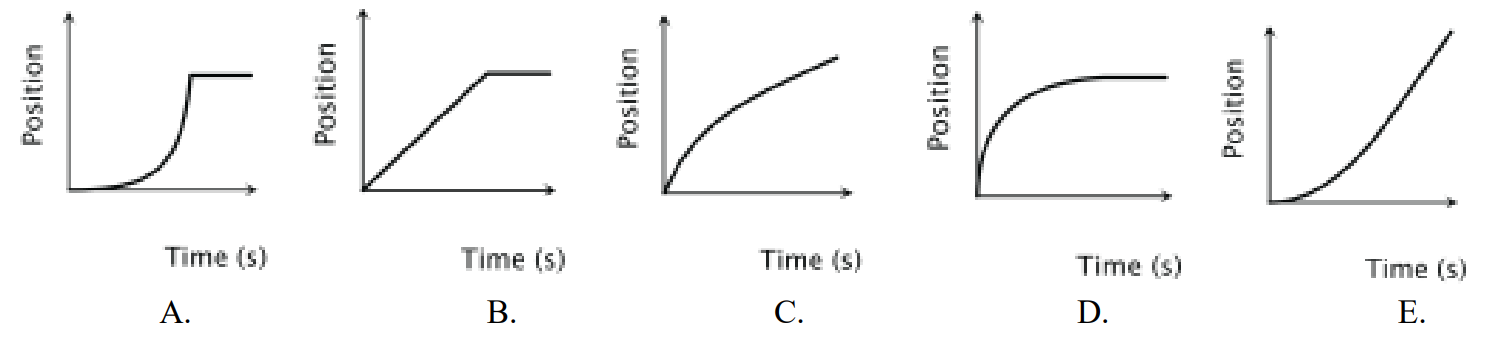
\includegraphics[width=\linewidth]{2018q10.png}\\
Ans: \ifpaper E \fi\\
\end{samepage}


\subsubsection{SJPO 2018 General Round Q16 \& Q17}
Lecture: \url{https://youtu.be/5M1mQjZJWI4} \\[10pt]
A car travels along a straight road with the speed shown by the 
v-t graph. \\ 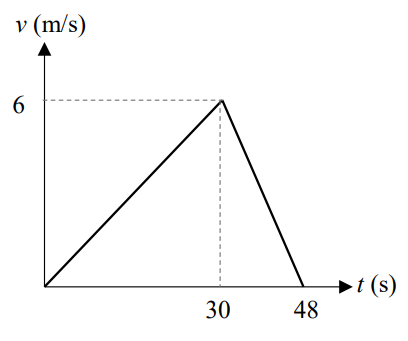
\includegraphics[width=0.5\linewidth]{images/2018q16.png} \\
\\
\begin{samepage}
16. What is the acceleration of the car from $t=30$ to $t=48 \mathrm{~s}$ ?
\begin{itemize}
\item[] (A) $-54 \mathrm{~m} / \mathrm{s}^2$ 
\item[] (B) $\quad 48 \mathrm{~m} / \mathrm{s}^2$ 
\item[] (C) $-3.0 \mathrm{~m} / \mathrm{s}^2$ 
\item[] (D) $\quad 3.0 \mathrm{~m} / \mathrm{s}^2$
\item[] (E) $-0.33 \mathrm{~m} / \mathrm{s}^2$\end{itemize}
Ans: \ifpaper E \fi
\end{samepage}
\\[20pt]
\begin{samepage}
17. What is the total displacement of the car after $48 \mathrm{~s}$ ?
\begin{itemize}
\item[] (A) $36 \mathrm{~m}$
\item[] (B) $48 \mathrm{~m}$
\item[] (C) $144 \mathrm{~m}$
\item[] (D) $180 \mathrm{~m}$
\item[] (E) $210 \mathrm{~m}$ 
\end{itemize}
Ans: \ifpaper C \fi\\
\end{samepage}
\\
\begin{samepage}
\subsubsection{SJPO 2017 General Round Q1} 
Lecture: \url{https://youtu.be/TW3sIS0lprI} \\[10pt]
An electron in a vacuum, starting from rest falls $5 \mathrm{~cm}$ near the surface of the earth. Considering only the gravitational force acting on the electron, how long does it take for the electron to travel $5 \mathrm{~cm}$?
\begin{itemize}
\item[] (A) $\quad 0.1 \mathrm{~s}$
\item[] (B) $\quad 0.03 \mathrm{~s}$
\item[] (C) $\quad 0.01 \mathrm{~s}$
\item[] (D) $\quad 0.001 \mathrm{~s}$
\item[] (E) $\quad 0.0001 \mathrm{~s}$
\end{itemize}
Ans: \ifpaper A \fi
\end{samepage}
% SJPO 2018 General Round Q18 C

\subsection{1D Dynamics}
Lecture: \url{https://youtu.be/xWJjy_5M4lA} \\[10pt]
If we know the acceleration as a function of time $a(t)$, as well as the initial velocity $v(t=0) \equiv v_0$ and position $s(t=0) \equiv s_0$, then we can integrate $a(t)$ twice to get the position as a function of time 
$$s(t) = \int \left(\int a(t)\ dt\right)\ dt$$

To obtain this $a(t)$, we use Newton's 2nd law 
$$F_{\text{net}}(t) = \frac{d(mv)}{dt} = m \frac{dv}{dt} + v \frac{dm}{dt}$$
In (most) cases where $m(t)$ is a constant wrt time, 
$$F_{\text{net}}(t) = ma(t)$$



\subsection{Extra: $v^2 = u^2 + 2as$ Connection with Work Energy Theorem}
Lecture: \url{https://youtu.be/1Z9V-1STA_Y} \\[10pt]
$v^2 = u^2 + 2as$ is slightly special because it is related to "work energy theorem" in dynamics. One can derive it by integrating $a(t)$ wrt $s(t)$ instead of $t$ 
\begin{align}
    \frac{d^2 s}{dt^2} &= a_0 \\
    \frac{d}{dt} \left(\frac{ds}{dt}\right) \frac{ds}{dt} dt &= a_0 ds \\
    \frac{1}{2} \frac{d}{dt} \left( v(t)^2 \right) dt &= a_0 ds \\
    \int_{t_A}^{t_B} \frac{1}{2} \frac{d}{dt} \left( v(t)^2 \right) dt &= \int_{s_A}^{s_B} a_0 ds \\
    \int_{v_A}^{v_B} \frac{1}{2} d\left( v^2 \right) &= a_0 (s_B - s_A) \\
    \frac{1}{2} (v_B^2 - v_A^2) &= a_0 (s_B - s_A) \\
    v_B^2 &= v_A^2 + 2a_0(s_B - s_A)
\end{align}

where we identify $v_B \equiv v$, $v_A \equiv u$, $s_B \equiv s$, $s_A \equiv 0$, $a_0 \equiv a$ to match \ref{eq:vuas}.
\\
 

\section{Math: 3D Vectors}

I made some H2 math videos on vectors 
\begin{itemize}
    \item \url{https://youtu.be/zohpKrmHkc0} Adding, scaling, subtraction of vectors
    \item \url{https://youtu.be/LhXac_HUw-0} Dot product
    \item \url{https://youtu.be/1qruXfQRQJU} Cross product
\end{itemize}
\leavevmode \\
In order to describe 3D motion we have 3 functions $x(t),y(t),z(t)$. To avoid writing three equations, we often package them into a position vector.
\begin{align}
    \vec{r}(t) = \left(
    \begin{array}{c}  
         x(t) \\
         y(t) \\
         z(t)
    \end{array}
    \right)
\end{align}

Geometrically, a vector can be thought of as an arrow. It is the "displacement between 2 points in 3D space", and points in a particular \textbf{direction} and has a \textbf{length/magnitude}. 

\subsection{Vector Operations}
\subsubsection{Adding}
Algebraically, just add each component individually
$$\left(
    \begin{array}{c}  
         x_1 \\
         y_1 \\
         z_1
    \end{array}
    \right) + \left(
    \begin{array}{c}  
         x_2 \\
         y_2 \\
         z_2
    \end{array}
    \right) = \left(
    \begin{array}{c}  
         x_1 + x_2 \\
         y_1 + y_2 \\
         z_1 + z_2
    \end{array}
    \right) 
$$
Geometrically, \\
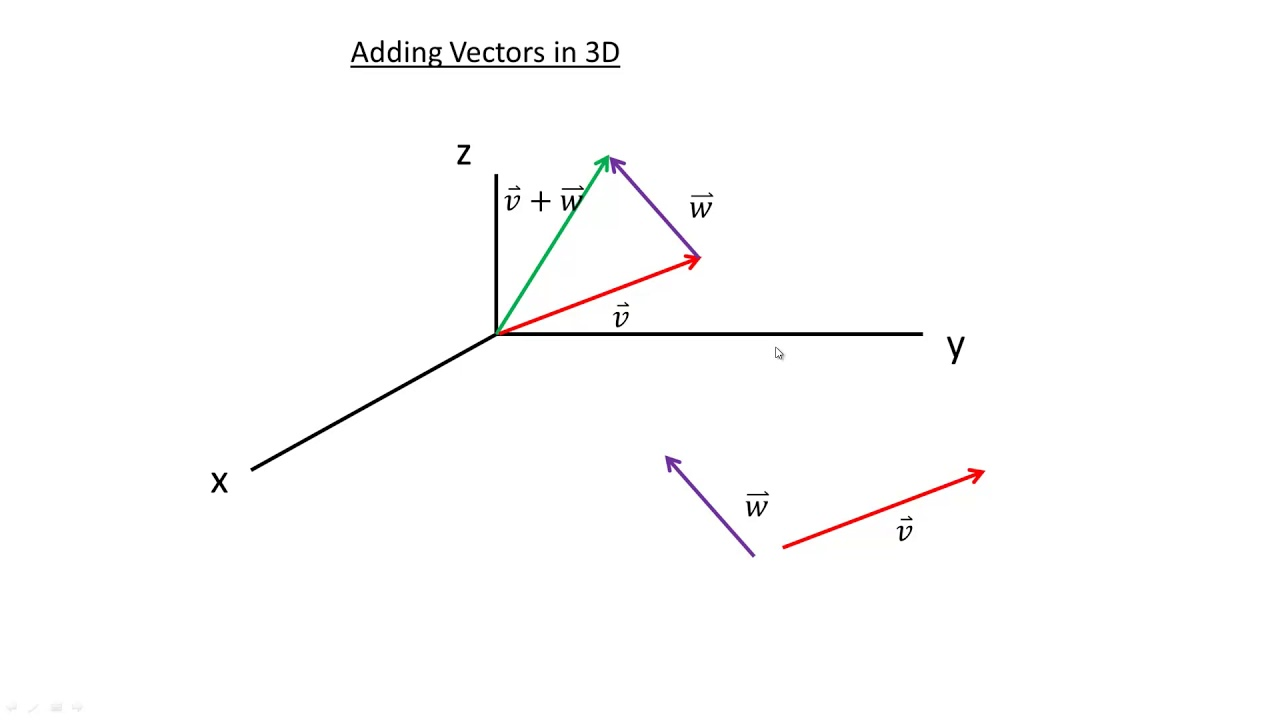
\includegraphics[width=\linewidth]{images/addingvectors.jpg}
\subsubsection{Scaling}
Algebraically, scale each component individually
$$
\lambda \left(
    \begin{array}{c}  
         x \\
         y \\
         z
    \end{array}
    \right) = \left(
    \begin{array}{c}  
         \lambda x \\
         \lambda y \\
         \lambda z
    \end{array}
    \right)
$$

Geometrically, if you scale a vector by a positive real number, direction stays the same but length is changed. \\
\begin{center}
    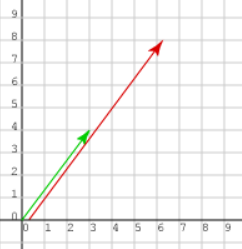
\includegraphics[width=0.3\linewidth]{images/scalingvector.png}
\end{center}
If scaled by a negative number, the direction flips (and length changes too).

\subsubsection{Length}
Algebraically, length is calculated using Pythagoras' theorem.
$$\left| \left(
    \begin{array}{c}  
         x \\
          y \\
          z
    \end{array}
    \right) \right| = \sqrt{x^2 + y^2 + z^2}
    $$

\subsubsection{Dot Product}
Dot product takes 2 vectors and outputs a single real number.
$$\left(
    \begin{array}{c}  
         x_1 \\
         y_1 \\
         z_1
    \end{array}
    \right) \cdot \left(
    \begin{array}{c}  
         x_2 \\
         y_2 \\
         z_2
    \end{array}
    \right) = x_1 x_2 + y_1 y_2 + z_1 z_2 
$$
Geometrically, dot product is a measure of how similar the direction of the 2 vectors are.
$$\vec{a} \cdot \vec{b} = |\vec{a}| |\vec{b}| \cos \theta $$
where $\theta$ is the angle between the 2 vectors.\\[10pt]
The dot product is used to define 
\begin{itemize}
    \item Work Done $W.(D) = \int \vec{F} \cdot d\vec{r}$
    \item Magnetic Flux $\Phi = \int \vec{B} \cdot d\vec{A}$
\end{itemize}

\subsubsection{Cross Product}
Cross product takes 2 vectors and outputs another vector.
$$\left(
    \begin{array}{c}  
         x_1 \\
         y_1 \\
         z_1
    \end{array}
    \right) \times \left(
    \begin{array}{c}  
         x_2 \\
         y_2 \\
         z_2
    \end{array} 
    \right) = \left(
    \begin{array}{c}  
         y_1 z_2 - z_1 y_2 \\
         z_1 x_2 - x_1 z_2 \\
         x_1 y_2 - y_1 x_2
    \end{array}
    \right)
$$

Geometrically, the length of the cross product is the area of the parallelogram. The direction of the cross product is perpendicular (following right hand rule). \\
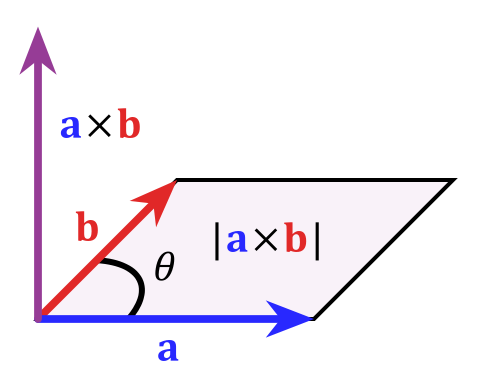
\includegraphics[width=0.49\linewidth]{images/crossproduct.png}
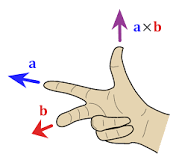
\includegraphics[width=0.49\linewidth]{images/crossproduct2.png}\\
The cross product is used to define 
\begin{itemize}
    \item Torque $\vec{\tau} = \vec{r} \times \vec{F}$
    \item Angular Momentum $\vec{L} = \vec{r} \times \vec{p}$
    \item Lorentz Force $\vec{F} = q(\vec{E} + \vec{v}\times \vec{B})$
    \item Poynting Vector $\vec{S}=\frac{1}{\mu_0} \vec{E} \times \vec{B}$
\end{itemize}
\subsubsection{Derivatives}
Also done component wise
$$\frac{d\vec{r}}{dt} = \frac{d}{dt}\left(
    \begin{array}{c}  
         x \\
         y \\
         z
    \end{array} 
    \right) = \left(
    \begin{array}{c}  
         dx/dt \\
         dy/dt \\
         dz/dt
    \end{array} 
    \right)
$$
\subsection{Basis Vectors}
We sometimes write a vector as 
\begin{align}
    \vec{r} &= \left(
    \begin{array}{c}  
         x(t) \\
         y(t) \\
         z(t)
    \end{array} 
    \right) \\
    &= x(t) \left(
    \begin{array}{c}  
         1 \\
         0 \\
         0
    \end{array} 
    \right) + y(t) \left(
    \begin{array}{c}  
         0 \\
         1 \\
         0
    \end{array} 
    \right) + z(t) \left(
    \begin{array}{c}  
         0 \\
         0 \\
         1
    \end{array} 
    \right)  \\
    &\equiv x(t) \hat{i} + y(t) \hat{j}  + z(t) \hat{k} 
\end{align}
Common synonyms for $\hat{i}$ are $\hat{x}$ and $\hat{e}_x$. The collection of vectors $\{ \hat i, \hat j, \hat k \}$ are called a set of \textbf{basis vectors}, which means that linear combinations of these vectors make up / span the set of all possible vectors. In particular, this set $\{ \hat i, \hat j, \hat k \}$ is called the \textbf{Cartesian coordinate basis}. In future, we will learn about other coordinate systems and other basis vectors.
\subsection{Exercises}
\begin{samepage}
\subsubsection{SJPO 2015 General Round Q11}
A force $\vec{F} = \vec{F}_1 + \vec{F}_2$ can be decomposed as the sum of 2 vectors $\vec{F}_1$ and $\vec{F}_2$. Only the magnitude of $\vec{F}_1$ and the direction of $\vec{F}_2$ are known. Which of the following is the most accurate statement?
\begin{itemize}
\item[](A) Only one combination of $\vec{F}_1$ and $\vec{F}_2$ exists.
\item[](B) There exists exactly two combinations of $\vec{F}_1$ and $\vec{F}_2$.
\item[](C) There exists infinite combinations of $\vec{F}_1$ and $\vec{F}_2$.
\item[](D) At least three combinations of $\vec{F}_1$ and $\vec{F}_2$ exist but the total number of combinations is finite.
\item[](E) Only one or two combinations of $\vec{F}_1$ and $\vec{F}_2$ exist.
\end{itemize}
Ans: \ifpaper E \fi
\end{samepage}
\begin{samepage}
\subsubsection{SJPO 2016 General Round Q21}
Initially, a $1\mathrm{~kg}$ box was sliding on frictionless surface at a constant velocity of $4\mathrm{~ms}^{-1}$ in the $\mathrm{x}$ direction. A constant force of $1\mathrm{~N}$ was applied on the box in a fixed direction for a time duration of $5\mathrm{~s}$. After $5\mathrm{~s}$ the speed of the box is $3\mathrm{~ms}^{-1}$. What is the magnitude of the change in momentum of the box?
\begin{itemize}
\item[](A) $1 \mathrm{kgms}^{-1}$
\item[](B) $2 \mathrm{kgms}^{-1}$
\item[](C) $3 \mathrm{kgms}^{-1}$
\item[](D) $4 \mathrm{kgms}^{-1}$
\item[](E) $5 \mathrm{kgms}^{-1}$
\end{itemize}
Ans: \ifpaper E \fi \\[10pt]
Extra: What are the possible directions of the applied force? 
\end{samepage}
\newpage
\section{Physics: Newtonian Mechanics}
The following quantities are scalars (real numbers)
\begin{itemize}
    \item mass $m$
    \item speed $|\vec{v}|$
    \item kinetic energy $E = \frac{1}{2} m|\vec{v}|^2$
    \item potential energy $U$
\end{itemize}
The following quantities are vectors
\begin{itemize}
    \item position $\vec{r}(t)$
    \item velocity $\vec{v}(t) \equiv \frac{d\vec{r}}{dt}$
    \item acceleration $\vec{a}(t) \equiv \frac{d^2\vec{r}}{dt^2}$
    \item force $\vec{F}(t)$
    \item momentum $\vec{p}(t) \equiv m\vec{v}(t)$
\end{itemize}
\leavevmode \\
\subsection{Newton's Three Laws}
\url{https://youtu.be/M6uYi0lcOvU}
Newton's 1st law defines what an inertial reference frame is: \textbf{In an inertial reference frame}, an object at rest remains at rest, or if in motion, remains in motion at a constant velocity unless acted on by a net external force.\\[10pt]
\textbf{In an inertial reference frame}, Newton's 2nd law
$$\vec{F}_{\text{net}} = \frac{d(m\vec{v})}{dt}$$
Newton's 3rd law 
$$\vec{F}_{\text{A on B}}(t) = -\vec{F}_{\text{B on A}}(t)$$

\subsection{Momentum \& Impulse}
\label{sec:momimp}
\url{https://youtu.be/TiOSscc8TKw}
Change in a particle's momentum is equal to the impulse it experiences. \\[10pt]
Newton's 2nd law: Let $\vec{F}(t)$ be the net force on a particle, then
$$\vec{F}(t) = \frac{d\vec{p}}{dt}$$
Let's focus on one component of the vector equation (say $F_x, p_x$)
$$F_x(t) = \frac{dp_x}{dt}$$
Integrating both sides wrt time $t$ from $t=t_A$ to $t=t_B$ yields

\begin{align}
    \int_{t_A}^{t_B} F_x(t) dt &= \int_{t_A}^{t_B} \frac{dp_x}{dt} dt \\
    \int_{t_A}^{t_B} F_x(t) dt &= \int_{p_x(t_A)}^{p_x(t_B)} dp_x \\
    &= p_x(t_B) - p_x(t_A) \\
    &= \Delta p_x
\end{align}
If a particle experiences a force $\vec{F}(t)$ over a time period $t_A$ to $t_B$, it's ($x$-component of) momentum will change by $\Delta p_x = \int_{t_A}^{t_B} F_x(t) dt$.\\[10pt]
This is true for each component $x,y,z$ so actually it is a vector equation 
$$\Delta \vec{p} = \int_{t_A}^{t_B} \vec{F}(t) dt$$
The quantity on the right hand side is called \textbf{impulse}.

\subsection{Kinetic Energy \& Work}
\url{https://youtu.be/DYRDr_ADIAM}
Often in physics, it is unnecessary to know the exact path $x(t)$ of a particle. Sometimes, the question only requires us to know $v(t)$. \\[10pt]
Example: A particle of mass $m$ experiences a force $F(x(t)) = \frac{A}{x(t)^2}$. It starts at $x(0)=x_0,\ x_0 > 0$ with an initial speed of $v_0$ toward $x=0$. Where will the particle come to a rest? \\[10pt]
One way of solving this is to find the function $x(t)$ that satisfies $F=ma$
$$\frac{A}{x^2} = m \frac{d^2x}{dt^2}$$
This is a differential equation, which we will cover later. We realise we cannot integrate wrt $t$ because the LHS itself is a function of $t$ we do not know the expression for. We will actually integrate wrt $x(t)$. We need to massage the equation into a different form first.\\[10pt]
By chain rule,
\begin{align}
\frac{d}{d t}\left[\left(\frac{d x}{d t}\right)^2\right]&=2  \frac{d x}{d t} \frac{d^2 x}{d t^2} 
\end{align}
Substituting this back in and simplifying
\begin{align}
\frac{A}{x^2}&=\frac{m}{2 \frac{d x}{d t}} \frac{d}{d t}\left[\left(\frac{d x}{d t}\right)^2\right] \\
& =\frac{m}{2} \frac{d}{d x}\left[\left(\frac{d x}{d t}\right)^2\right] \\
& =\frac{m}{2} \frac{d}{d x} v^2 
\end{align}
Then integrating from the starting to the stopping point wrt $x$ instead of $t$,
\begin{align} 
\int_{x_0}^{x_{\text {stop }}} \frac{A}{x^2} d x&=\frac{m}{2} \int_{v_0^2}^{v_{\text {stop }}^2=0} d\left[\left(\frac{d x}{d t}\right)^2\right] \\
\left[-\frac{A}{x}\right]_{x_0}^{x_\text{stop}} &= \left[\frac{1}{2} m v^2\right]_{v^2=v_0^2}^{v^2=0} \\
\frac{A}{x_0}-\frac{A}{x_\text {stop }}&=-\frac{1}{2} m v_0^2 \\
\frac{A}{x_0}+\frac{1}{2} m v_0^2&=\frac{A}{x_\text {stop }} \label{eq:pepke}\\
x_{\text{stop}} &= A \left(\frac{A}{x_0}+\frac{1}{2} m v_0^2\right)^{-1}
\end{align}
The left hand side of Equation \ref{eq:pepke} is actually potential energy + kinetic energy. We will talk about potential energy in future, but for now we observe that integrating $F$ with respect to $x$ instead of $t$ was a useful trick. Generalizing this to a general force $F$,

\begin{align}
    F &= ma \\
    \int_{x_A}^{x_B} F dx &= m \int_{x_A}^{x_B} a dx 
\end{align}
Claim: $a\ dx = v\ dv$. Proof: 
\begin{align}
v\ dv
& = \frac{1}{2} d\left(v^2\right) \\
& =\frac{1}{2} \frac{d}{d t}\left(v^2\right) d t \\
& =\frac{1}{2} 2 v a\ d t \\
& =a\ v\ d t \\
& =a \ d x
\end{align}
So by a change in variables, $a\ dx = v\ dv$. 
\begin{align}
    \int_{x_A}^{x_B} F dx &= m \int_{x_A}^{x_B} a dx \\
    &= m \int_{v_A}^{v_B} v dv \\
    &= \frac{1}{2} m \left[v^2\right]_{v_A}^{v_B} \\
    &= \frac{1}{2} m v_B^2 - \frac{1}{2} mv_A^2 \\
    &= \Delta K.E.
\end{align}
In other words, if a particle experiences a force $F(x)$ over a distance interval from $x_A$ to $x_B$, it's change of kinetic energy $\Delta\left(\frac{1}{2}mv^2\right)$ is given by $$\Delta K.E. = \int_{x_A}^{x_B} F(x)\ dx$$
which we call the \textbf{work done} on the particle. This is the \textbf{Work Energy theorem}.\\[10pt]
Extra: Mathematically, what we have actually done is we have transformed a 2nd order ODE $a(x)$ into a 1st order ODE $v(x)$, which should be easier to integrate in general.

\section{Physics: Projectile Motion}
\url{https://youtu.be/-Yq6wzXTU84}
\begin{align}
\vec{F}_{\text{net}} &= m \vec{a} \\
\Rightarrow \left(
    \begin{array}{c}  
         0 \\
         -mg \\
         0
    \end{array} 
    \right) &= m \left(
    \begin{array}{c}  
         d^2x/dt^2 \\
         d^2y/dt^2 \\
         d^2z/dt^2
    \end{array} 
    \right)
\end{align}
Integrating twice with respect to time $t$,
\begin{align}
    \left(
    \begin{array}{c}  
         x(t) \\
         y(t) \\
         z(t)
    \end{array} 
    \right) = \left(
    \begin{array}{c}  
          {u}_x t + {r_0}_x\\
         -\frac{1}{2}gt^2 + {u}_y t + {r_0}_y\\
          {u}_z t + {r_0}_z
    \end{array} 
    \right)
\end{align}
We need to know the initial position $\vec{r}_0 \equiv \vec{r}(t=0)$ and initial velocity $\vec{u} \equiv \vec{v}(t=0)$. For example, 
\begin{align}
    \vec{r}(t=0) &= \left(
    \begin{array}{c}  
         0 \\
         0 \\
         0
    \end{array} 
    \right) \\
    \vec{v}(t=0) &= \left(
    \begin{array}{c}  
         u \cos \theta \\
         u \sin \theta \\
         0
    \end{array} 
    \right)
\end{align}   
Then that gives us the path of the projectile with respect to time
\begin{align}
    x(t) &= u \cos \theta\ t \label{eq:xt} \\
    y(t) &= u \sin \theta\ t - \frac{1}{2} gt^2 \\
    z(t) &= 0
\end{align}
This is also known as a parametric curve, with time $t$ being the parameter. Every value of $t$ gives us a point in space $(x(t),y(t),z(t))$. 

\subsection{From parametric to $y(x)$}
\url{https://youtu.be/IfFNoepeMow}
If we want to convert parametric curve into a formula for the graph $y(x)$, then we need to invert Equation \ref{eq:xt} to yield $$t(x) = {\frac{x}{u \cos \theta}}$$
Substituting $t(x)$ into $y(t)$ gives us $y(x)$
\begin{align}
    y(x) &= \tan \theta\ x - \frac{g}{2u^2 \cos^2 \theta} x^2
\end{align}
\subsection{Finding Range}
There are 2 solutions to $y(x) = 0$: the starting one being $x_{\text{start}}=0$. The other is 
$$x_{\text{end}} = \frac{2u^2}{g} \sin \theta \cos \theta = \frac{u^2}{g} \sin 2\theta$$

We now have range as a function of angle $x_{\text{end}}(\theta)$. We can differentiate this with respect to $\theta$ and set the derivative $dx_{\text{end}}/d\theta = 0$ to find the maximum range. Strictly speaking, we have to check the second derivative too.
% \subsubsection{Region of Reachability}
\subsection{Exercises}
\begin{samepage}
\subsubsection{SJPO 2016 General Round Q9}
\url{https://youtu.be/gBjapzk5Tws}\\[10pt]
A fruit drops from a tree. A boy, $1.5 \mathrm{~m}$ tall, stands on the flat ground just under the fruit. The fruit was initially $10 \mathrm{~m}$ above the boy's head. A woman standing on the level ground $10 \mathrm{~m}$ from the boy immediately throws a ball from a height of $1.5 \mathrm{~m}$ above the ground, and deflected the fruit from its path towards the boy's head. Assume that air resistance and her reaction time are negligible. Calculate the minimum speed of the ball?
\begin{itemize}
\item[](A) $10 \mathrm{ms}^{-1}$
\item[](B) $15 \mathrm{ms}^{-1}$
\item[](C) $20 \mathrm{ms}^{-1}$
\item[](D) $25 \mathrm{ms}^{-1}$
\item[](E) $30 \mathrm{ms}^{-1}$
\end{itemize}
Ans: \ifpaper A \fi \\[10pt]
\end{samepage}

\begin{samepage}
\subsubsection{SJPO 2016 General Round Q11: Region of Reachability}
\url{https://youtu.be/axU4CSp8UqI}\\[10pt]
A projectile is launched at velocity $v_0$ into an ideal ball istic trajectory from the origin of a coordinate system. Given that: when the launch angle is varied, all the possible points that can be hit by the projectile are exactly contained within a parabola with equation $y=a+b x^2$ where $y$ is the vertical height, $x$ is the horizontal displacement from the origin, while $a$ and $b$ are constants. What could be the expression for $a$ and $b$ ?\\
 \begin{wrapfigure}{r}{0.4\textwidth} 
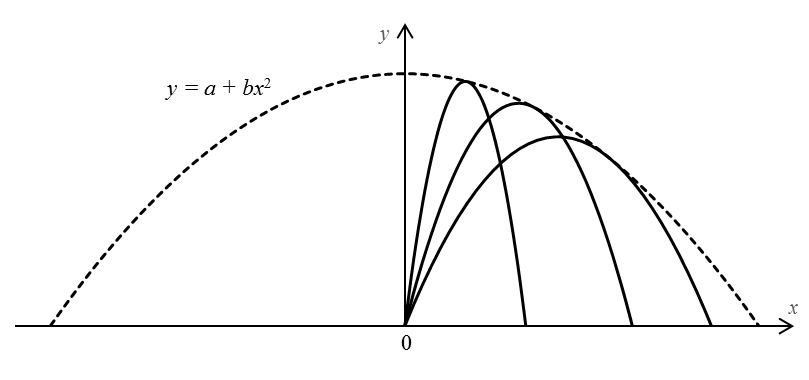
\includegraphics[width=\linewidth]{images/sjpo2016q11.png}
\end{wrapfigure}
\begin{itemize}
\item[](A) $\quad a=\frac{v_0{ }^2}{2 g}, b=\frac{g}{v_0{ }^2}$
\item[](B) $\quad a=\frac{v_0{ }^2}{2 g}, b=\frac{g}{2 v_0{ }^2}$
\item[](C) $\quad a=\frac{v_0{ }^2}{2 g}, b=\frac{2 g}{v_0{ }^2}$
\item[](D) $\quad a=\frac{v_0{ }^2}{g}, b=-\frac{g}{v_0{ }^2}$
\item[](E) $\quad a=\frac{v_0{ }^2}{2 g}, b=-\frac{g}{2 v_0{ }^2}$
\end{itemize}
Ans: \ifpaper E \fi \\[10pt]
Extra: Prove that the envelope is a parabola. \url{https://en.wikipedia.org/wiki/Envelope_(mathematics)}
\end{samepage}

\begin{samepage}
\subsubsection{SJPO 2014 General Round Q12: Projectile on Slope}
\url{https://youtu.be/l4lq6dXTug0}\\[10pt]
As shown in the figure below, a ball is thrown out horizontally from a slope. The slope makes an angle $\theta$ with the ground. At the first throw, the ball is ejected with a speed $v_1$ and at the second throw, it is ejected with a speed $v_2$. The angles that the ball made with the slope are measured to be $\alpha_1$ and $\alpha_2$ respectively. If $v_1$ is greater than $v_2$,\\
 \begin{wrapfigure}{r}{0.4\textwidth} 
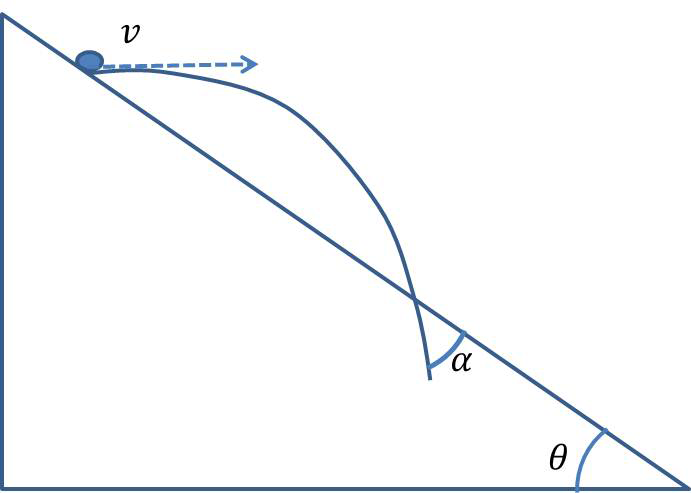
\includegraphics[width=\linewidth]{images/2014q12.png}
\end{wrapfigure}
\begin{itemize}
\item[](A) $\alpha_1=\alpha_2$
\item[](B) $\alpha_1>\alpha_2$
\item[](C) $\alpha_1<\alpha_2$
\item[](D) $\alpha<\theta$
\item[](E) It is not possible to infer much as the mass of the ball is not given.
\end{itemize}
Ans: \ifpaper A \fi \\[10pt]
\end{samepage}



% Hitting a slope\\
% Starting from a height \\
% Minimum velocity to cross a wall (spot)\\
% (ODE) With air resistance

\section{Physics: Constraining Forces}
\label{sec:fnt}
Constraint forces are generally forces that will \textbf{adjust} their magnitude to \textbf{prevent some form of motion}. For example, normal contact force prevents objects from sinking into each other. Friction prevents rough objects from sliding with respect to each other. And tension in an inextensible string limits the distance between two objects. 
\subsection{Normal Contact Force}
Normal contact force $N$ between two rigid bodies \textbf{in contact} is a vector:
\begin{itemize}
    \item Direction: Always normal to the surfaces in contact, opposes "sinking"
    \item Magnitude: can range from $0$ to $\infty$. If magnitude is $0$, the two bodies is about to \textbf{lose contact}.
\end{itemize}
Normal contact force obeys N3L.
\subsection{Friction}
Frictional force between two rough bodies \textbf{in contact} is a vector: 
\begin{itemize}
    \item Direction: Always parallel to the surfaces in contact, opposes sliding
    \item Magnitude: can range from $|F_{\text{fric}}| \leq \mu_s N$. If friction is maxed out at $\mu_s N$, it will soon be unable to counteract the external forces, and the two bodies will \textbf{start sliding}.
\end{itemize}
$\mu_s$ is the static coefficient of friction. \\[10pt]
When sliding starts, the magnitude will be limited by the kinetic coefficient of friction $\mu_k$ instead of $\mu_s$. Usually $\mu_k < \mu_s$, which is why you will lose control of your car if your tyres skid.

\subsubsection{SJPO 2015 General Round Q12}
\label{sec:sjpo2015q12sec_static}
As shown in the figure below, the block with mass $M$ is stationary upon the plank and the angle of the slope $\theta$ is increased. Which of the following is true for the normal force of the block on the wooden plank, $N$ and the frictional force on the plank, $f$? \\
\begin{wrapfigure}{r}{0.36\textwidth}
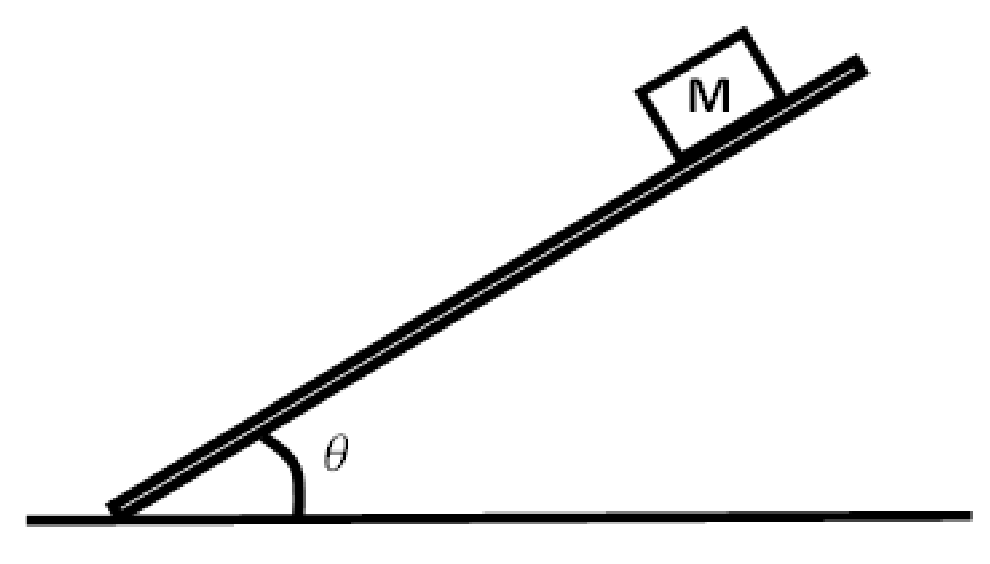
\includegraphics[width=1.0\linewidth]{images/sjpo2015q12.png}
\end{wrapfigure}


\begin{itemize}
\item[] (A) Both $N$ and $f$ increase.
\item[] (B) Both $N$ and $f$ decrease.
\item[] (C) $N$ increases and $f$ decreases.
\item[] (D) $N$ decreases and $f$ increases.
\item[] (E) The response differs when the value of $M$ is different.
\end{itemize}
Ans: \ifpaper D \fi \\[10pt]
Extra: If the static coefficient of friction is $\mu$, at what angle $\theta_{\text{max}}$ does the block begin slipping?



\subsubsection{SJPO 2016 General Round Q4}
A box is pulled using a string up a 0.1 radian slope at constant speed of $2.0 \mathrm{~ms}^{-1}$. The string is cut suddenly and the box comes to a stop after moving up a further distance of $1.0 \mathrm{~m}$. What is the value of the coefficient of friction?
{
\begin{wrapfigure}{r}{0.6\textwidth}
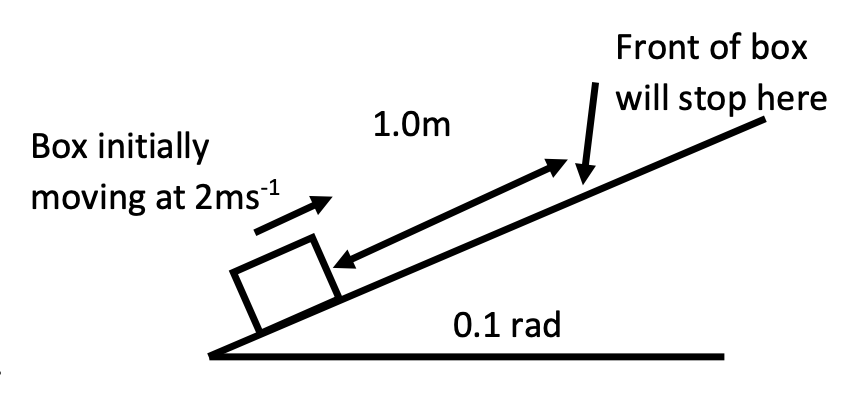
\includegraphics[width=1.0\linewidth]{images/sjpo2016q4.png}
\end{wrapfigure}
\begin{itemize}
\item[] (A) $\quad 0.00$
\item[] (B) $\quad 0.10$
\item[] (C) $\quad 0.20$
\item[] (D) $\quad 0.30$
\item[] (E) The situation is impossible.
\end{itemize}
}
Ans: \ifpaper B \fi
\subsection{Tension}
Tension in the string connecting two bodies is a vector:
\begin{itemize}
    \item Direction: \textbf{Isotropic} and constant anywhere \textbf{along the string}. Parallel and toward the string at \textbf{endpoints of string}.
    \item Magnitude: can range from $0$ to $\infty$, unless question specifies a limit. If the tension is $0$, the string is loose.
\end{itemize}
For a massless string (whether straight or curved on a pulley), tension is equal everywhere along the string (can be easily proven). This is particular useful for pulley questions. \\[10pt]
We will deal with massive string after talking about "mass distributions" (Topic of Moment of Inertia).\\[10pt]
Extra: A string on a pulley with friction has an exponential effect in increasing tension. See \url{https://en.wikipedia.org/wiki/Capstan_equation}. We will cover this in future too.

\subsubsection{SJPO 2014 General Round Q41}
A block of mass $m$ is attached to a horizontal inextensible string and is moving upwards as shown in the figute below. Breaking strength of the string is $4 \mathrm{mg}$. The maximum positive and negative accelerations that the block can have are
{
\begin{wrapfigure}{r}{0.4\textwidth}
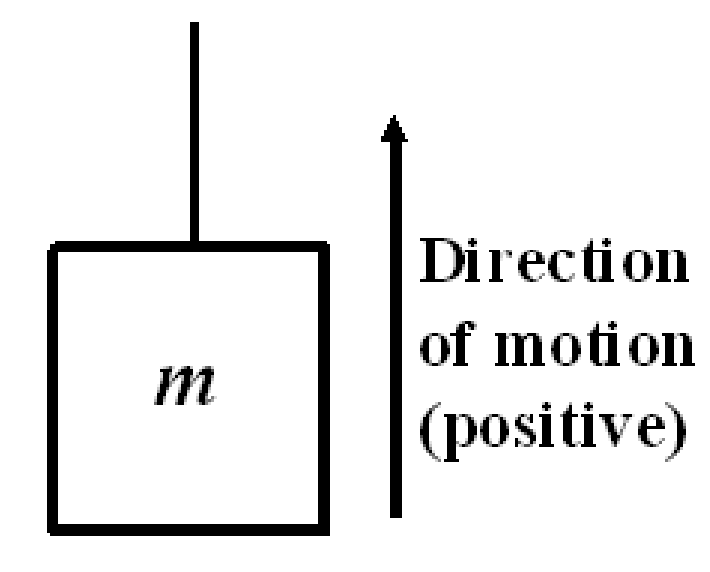
\includegraphics[width=1.0\linewidth]{images/sjpo2014q41.png}
\end{wrapfigure}

\begin{itemize}
\item[] (A) $4 \mathrm{~g}$ and $3 \mathrm{~g}$ respectively.
\item[] (B) $4 \mathrm{~g}$ and g respectively.
\item[] (C) $3 g$ and $4 \mathrm{~g}$ respectively.
\item[] (D) $3 \mathrm{~g}$ and g respectively.
\item[] (E) $3 \mathrm{~g}$ and $3 \mathrm{~g}$ respectively.
\end{itemize}
}
Ans: \ifpaper D \fi
\clearpage
\subsubsection{SJPO 2018 General Round Q6}
\label{sec:sjpo2018q6sec_static}
\begin{wrapfigure}{r}{0.5\textwidth}
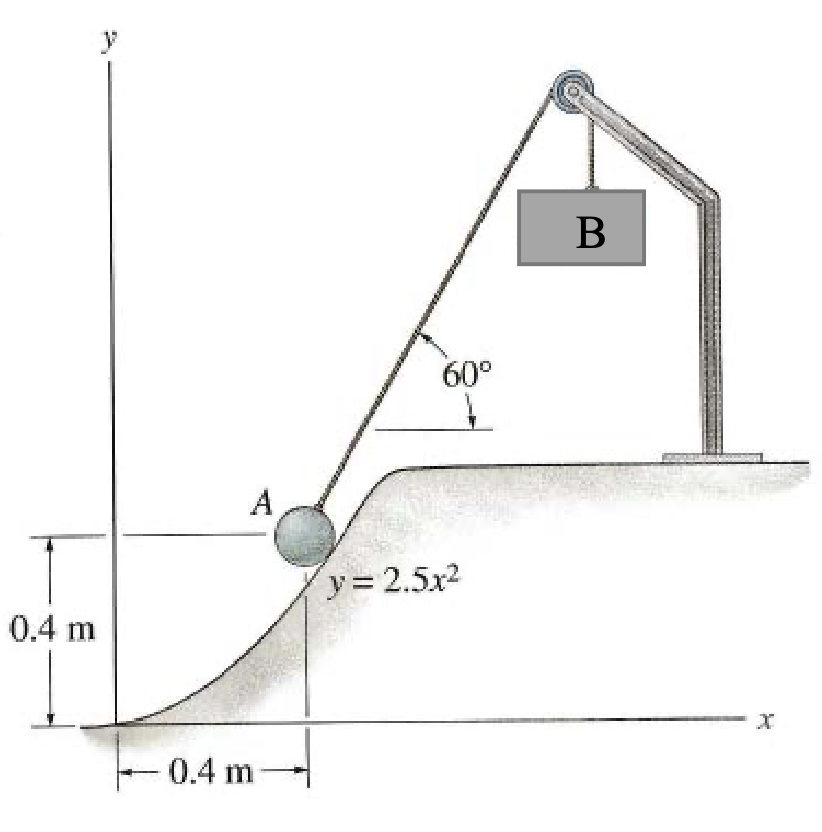
\includegraphics[width=1.0\linewidth]{images/sjpo2018q6.png}
\end{wrapfigure}
A $4 \mathrm{~kg}$ sphere rests on the smooth parabolic surface which is given by the equation $y=2.5 x^2$. The sphere just touches the surface at $(x, y)=(0.4 \mathrm{~m}, 0.4 \mathrm{~m})$. Determine the mass $m_{\mathrm{B}}$ of block B needed to hold the sphere in equilibrium.
\begin{itemize}
\item[] (A) $4.14 \mathrm{~kg}$
\item[] (B) $3.75 \mathrm{~kg}$
\item[] (C) $3.58 \mathrm{~kg}$
\item[] (D) $2.93 \mathrm{~kg}$
\item[] (E) $2.14 \mathrm{~kg}$
\end{itemize}
Ans: \ifpaper C \fi
\clearpage

\section{Physics: Drag / Air Resistance}

Drag is a force dependent on velocity and the \textbf{geometry} of the object.
\begin{align}
    F_{\text{drag}}(v) =\frac{1}{2} \rho v^2 C_D(v) A
\end{align}
\begin{itemize}
    \item $\rho$ is the density of the fluid
    \item $v$ is velocity of object relative to fluid
    \item $C_D(v)$ is dimensionless drag coefficient (usually obtained experimentally), which is a function of velocity
    \item $A$ is cross sectional area
\end{itemize}
At low velocities, $C_D(v) \propto 1/v$ approximately, so $F_{\text{drag}}(v) \propto v$ \\[10pt]
At high velocities, $C_D(v)$ is approximately constant, so $F_{\text{drag}}(v) \propto v^2$. \\[10pt]
In Physics Olympiad, the question will typically specify. \\[10pt]
Drag is the reason why falling objects have a terminal velocity
\subsection{Terminal Velocity}
(Taking the y-axis as downward positive), the net vertical forces on an object falling is
\begin{align}
    ma(t) = F_{\text{net}}(v) = mg - F_{\text{drag}}(v)
\end{align}
As $v(t)$ increases over time, drag force increases, causing $a(t)$ to decrease. The resultant motion is that $v(t)$ approaches asymptotically to a constant $v_{\text{terminal}}$, at which $$F_{\text{net}}(v_{\text{terminal}}) = 0$$

\subsection{Exercises}
\subsubsection{SJPO 2018 General Round Q2}
A tiny spherical raindrop of diameter $D=0.1 \mathrm{~mm}$ experiences a linear drag force while falling at speed $v$, given by $F_{\text {drag }}=c v$, where $c=1.55 \times 10^{-6} \mathrm{~N} \mathrm{~s} \mathrm{~m}^{-1}$. What is its terminal speed?
\begin{itemize}
\item[] (A) $1.7 \mathrm{~mm} / \mathrm{s}$
\item[] (B) $3.3 \mathrm{~mm} / \mathrm{s}$
\item[] (C) $8.5 \mathrm{~mm} / \mathrm{s}$
\item[] (D) $26 \mathrm{~mm} / \mathrm{s}$
\item[] (E) $33 \mathrm{~mm} / \mathrm{s}$
\end{itemize}
Ans: \ifpaper B \fi

\subsubsection{SJPO 2017 General Round Q7}
An object, \textbf{1}, with mass $m$ and another object, \textbf{2}, with twice the mass $2 m$ are dropped from rest, at the same starting position from the top of a large container and fall in a straight line through motionless viscous liquid. Drag is significant and assume that the two objects would eventually reach the same terminal velocity $v_T$ if the container were tall enough. Consider the case where the objects do not reach terminal velocity at the bottom of the container. Assume that the same type of drag acts on both objects. How does the time taken, $t_1$ and $t_2$, for the objects \textbf{1} and \textbf{2} to reach the bottom compare?\\[10pt]
{
 \begin{wrapfigure}{r}{0.5\textwidth} 
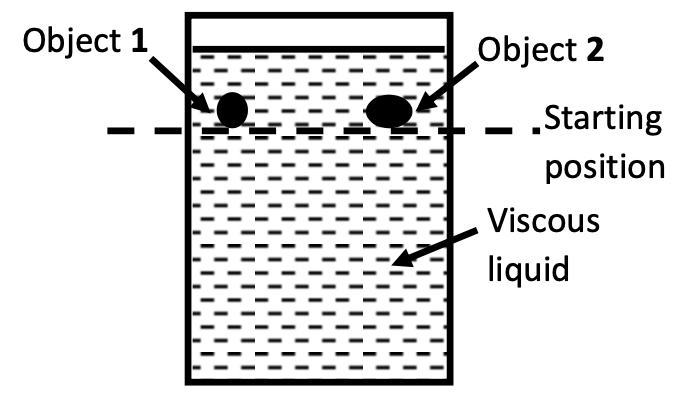
\includegraphics[width=\linewidth]{images/sjpo2016q7.png}
\end{wrapfigure}
\begin{itemize}
\item[] (A) $t_1=t_2$
\item[] (B) $t_1<t_2$
\item[] (C) $t_1>t_2$
\item[] (D) $t_2<t_1<2 t_2$
\item[] (E) $t_1<t_2<2 t_1$
\end{itemize}
}
Ans: \ifpaper A \fi


\subsection{Extra: Up and Down with Air Resistance}
In a case \textbf{without air resistance}, if we throw a ball up, suppose it takes $T_1$ seconds to reach the peak from the time it was released, and $T_2$ seconds to fall back down from the peak to the original point of release. One can prove $T_1 = T_2$ easily.\\[10pt]
In a case \textbf{with air resistance},
suppose the time to reach the peak is $\tau_1$ and the time to drop down is $\tau_2$. \textbf{Prove rigorously} that $\tau_1 < \tau_2$.\\[10pt]
\url{https://youtu.be/1uaHkc3TfBU}

\subsection{Extra: Projectile Motion with Drag}
It is possible to solve for projectile motion exactly, but only after we study differential equations. We postpone this to the future.
\newpage
\section{Physics: Collisions}
Collisions between multiple bodies (e.g. dropping a stack of balls) are analysed as a sequence of collisions between 2 bodies at a time. When 2 bodies collide, their \textbf{total momentum is always conserved} / invariant before and after the collision (invariant means doesn't change). Their total \textbf{kinetic} energy, however, has 3 possibilities:
\begin{itemize}
    \item Total KE conserved (\textbf{elastic})
    \item Total KE decreased (\textbf{inelastic}) e.g. billiard balls
    \item Total KE increased (\textbf{superelastic}) e.g. compressed spring, explosion
\end{itemize}
\subsection{Momentum Conservation}
\url{https://youtu.be/nJlILp1fBwI}\\
\textbf{Q}: Why is momentum invariant before and after the collision? \\[10pt]
\textbf{A}: Momentum conservation is due to Newton's 3rd Law. To see this, recall that an object's momentum changes by impulse 
$$\Delta \vec{p} \text{ from } t_0 \text{ to } t_1 = \int_{t_0}^{t_1} \vec{F}(t)\ dt$$
By Newton's 3rd Law, when 2 bodies interact, the forces they exert on each other are equal in magnitude and opposite in direction. 
$$\vec{F}_{\text{A on B}} = -\vec{F}_{\text{B on A}}$$
Integrating both sides wrt time $t$, one sees that the impulse they experience is also equal in magnitude and opposite in direction.
$$\Delta \vec{p}_B = - \Delta \vec{p}_A$$
As such, the sum of their momentum remains unchanged.
$$\Delta(\vec{p}_A + \vec{p}_B) = \vec{0}$$
This remains true for all forces that obey N3L, including collisions (normal contact force). 
\subsection{1D Elastic Collisions}
\url{https://youtu.be/iwPXjULdcuc}\\
Let the masses be $m_A, m_B$, the initial velocities be $u_A, u_B$ and final velocities be $v_A, v_B$. Conservation of momentum and energies yields
\begin{align}
    m_A u_A + m_B u_B &= m_A v_A + m_B v_B \\
    \frac{1}{2} m_A u_A^2 + \frac{1}{2} m_B u_B^2 &= \frac{1}{2} m_A v_A^2 + \frac{1}{2} m_B v_B^2 
\end{align}
Rearranging both equations gives us (respectively)
\begin{align}
    m_A (u_A - v_A) &= - m_B (u_B - v_B) \label{eq:com}\\
    m_A (u_A - v_A) (u_A + v_A) &= - m_B (u_B - v_B) (u_B + v_B) \label{eq:coe}
\end{align}
If we divide equation \ref{eq:coe} by \ref{eq:com} we obtain
\begin{align}
    u_A + v_A &= u_B + v_B \\
    \Rightarrow u_A - u_B &= - (v_A - v_B)
\end{align}
\begin{samepage}
This equation is sometimes said verbally as 
\begin{center}
    \textbf{velocity of approach = velocity of separation}
\end{center}
\end{samepage}
This is because if object A is positioned to the left of object B (and our choice of axis direction is rightward positive), then a positive $u_A - u_B > 0$ would imply that A is getting closer to B, and $u_A - u_B$ describes how fast the distance between them is decreasing. Hence, $u_A - u_B > 0$ is called the \textbf{velocity of approach}. \\[10pt]
After the collision, $v_A - v_B = -(u_A - u_B) < 0$ implies that B is getting further and further away from A. $-(v_A - v_B) > 0$ quantifies how fast the distance between them is increasing. Hence, $-(v_A - v_B) > 0$ is called the \textbf{velocity of separation}.\\[10pt]
Anyway, previously we had one linear equation (momentum) and one quadratic equation (energy). Now we have 2 linear equations (momentum and "rate of approach = separation")
\begin{align}
    m_A u_A + m_B u_B &= m_A v_A + m_B v_B \label{eq:com2}\\
    u_A - u_B &= - (v_A - v_B) \label{eq:voaevos}
\end{align}
Linear simultaneous equations are easy to solve, rearrange equation (\ref{eq:voaevos}) and substitute $v_A = v_B - u_A + u_B$ into (\ref{eq:com2}) to obtain
\begin{align}
    m_A u_A + m_B u_B &= m_A (v_B - u_A + u_B) + m_B v_B \\
    &= (m_A + m_B) v_B - m_A u_A + m_A u_B \\
    v_B &= \frac{2m_A}{m_A + m_B} u_A + \frac{m_B - m_A}{m_A + m_B} u_B 
\end{align}
Repeating this with $v_B = u_A - u_B + v_A$ gives us 
\begin{align}
    m_A u_A + m_B u_B &= m_A v_A + m_B (u_A - u_B + v_A) \\
    &= (m_A + m_B) v_A + m_B u_A - m_B u_B \\
    v_A &= \frac{m_A - m_B}{m_A + m_B} u_A + \frac{2m_B}{m_A + m_B} u_B
\end{align}
One sees that the final velocities almost look like they have a nice symmetry to them. You can memorise these formulas but personally I just derive it every time I need it because I don't like memorising.
\subsubsection{SJPO 2017 General Round Q40}
\url{https://youtu.be/IVkbicUsFrg}\\
40. A small tennis ball with mass $m$ sits atop a large basketball with mass $M$, with $M \gg m$. The balls are released from rest, with the bottom of the basketball at a height $\mathrm{h}$ above the ground. The diameter of the tennis ball is d and that of the basketball is $D$, with $D \gg d \approx 0$. To what height does the tennis ball bounce above the ground? Assume all collisions are elastic.
\begin{itemize}
\item[] (A) $D+h$
\item[] (B) $D+4 h$
\item[] (C) $D+8 h$
\item[] (D) $D+9 h$
\item[] (E) There is insufficient information.
\end{itemize}
Ans: \ifpaper D \fi
Extra: There is an extension of this to multiple balls in H3 physics \url{https://youtu.be/drVTrXib-7g?t=260}

\subsection{Center of Momentum Frame}
\url{https://youtu.be/Z28XlyN7WJ8}\\
The Center of Momentum frame (CoM) is very useful because it simplifies the momentum equation greatly. The CoM frame is defined to be the frame in which the total momentum is zero. So, in any dimension,
\begin{align}
    m_A \mathbf{u}_{A,CM} + m_B \mathbf{u}_{B,CM} &= m_A \mathbf{v}_{A,CM} + m_B \mathbf{v}_{B,CM} = \mathbf{0} \label{eq:zeromomentum}
\end{align}
where the bolded quantities $\mathbf{u}$ emphasise that this is a vector equation. We can show that such a frame exists by proof by construction 
\begin{align}
    \mathbf{u}_A &\equiv \mathbf{u}_{CM} + \mathbf{u}_{A,CM} \\
    \mathbf{u}_B &\equiv \mathbf{u}_{CM} + \mathbf{u}_{B,CM} \\
    \text{Define/Choose }\mathbf{u}_{CM} &= \frac{m_A \mathbf{u}_A + m_B \mathbf{u}_B}{m_A + m_B} \\
    m_A \mathbf{u}_{A,CM} + m_B \mathbf{u}_{B,CM} &= m_A (\mathbf{u}_A  - \mathbf{u}_{CM}) + m_B (\mathbf{u}_B - \mathbf{u}_{CM}) \\
    &= m_A \mathbf{u}_A + m_B \mathbf{u}_B - (m_A + m_B) \mathbf{u}_{CM} \\
    &= \mathbf{0}
\end{align}
Rearranging the zero total momentum equation (\ref{eq:zeromomentum}) yields A's velocities in terms of B's velocities
\begin{align}
    \mathbf{u}_{A,CM} &= -\frac{m_B}{m_A} \mathbf{u}_{B,CM} \label{eq:meow1}\\
    \mathbf{v}_{A,CM} &= -\frac{m_B}{m_A} \mathbf{v}_{B,CM} \label{eq:meow2}
\end{align}

\subsubsection{Elastic Collision in CoM Frame}
Equations (\ref{eq:meow1}) and (\ref{eq:meow2}) can be substituted into the conservation of KE equation to eliminate A's initial and final velocities, leaving us with an equation purely relating B's initial and final velocities
\begin{align}
    \frac{1}{2} m_A \mathbf{u}_{A}^2 + \frac{1}{2} m_B \mathbf{u}_{B}^2  &= \frac{1}{2} m_A \mathbf{v}_{A}^2 + \frac{1}{2} m_B \mathbf{v}_{B}^2 \\
    \Rightarrow \left( \frac{m_B^2}{m_A} + m_B \right) \mathbf{u}_{B,CM}^2 &= \left( \frac{m_B^2}{m_A} + m_B \right) \mathbf{v}_{B,CM}^2 \\
    \Rightarrow \mathbf{u}_{B,CM}^2 &= \mathbf{v}_{B,CM}^2 
\end{align}
\subsubsection{1D Elastic Collision Revisited using CoM Frame}
\url{https://youtu.be/gwpOOmzETX8}\\
The CoM equations become
\begin{align}
    m_A u_{A,CM} + m_B u_{B,CM} &= 0 \\
    m_A v_{A,CM} + m_B v_{B,CM} &= 0 \\
    u_{B,CM}^2 &= v_{B,CM}^2 
\end{align}
If B is to the right of A (and our axis is defined as rightward positive), then $u_{B,CM} < 0$ because B is moving left in the CM frame before the collision. $v_{B,CM} > 0$ because B is moving right in the CM frame after the collision. Hence 
\begin{align}
    u_{B,CM}^2 &= v_{B,CM}^2 \\
    \Rightarrow v_{B,CM} &= -u_{B,CM} \\
    v_{A,CM} &= -\frac{m_B}{m_A} v_{B,CM} \\ 
    &= \frac{m_B}{m_A} u_{B,CM} \\
    &= - u_{A,CM}
\end{align}
Wow! What a remarkably neat result. In the CoM frame, the velocities simply flip direction during the collision. Returning to the lab frame, we obtain 
\begin{align}
    v_A &= u_{CM} + v_{A,CM} \\
    &= u_{CM} - u_{A,CM} \\
    &= u_{CM} - (u_A - u_{CM}) \\
    &= 2 u_{CM} - u_A \\
    &= 2 \frac{m_A u_A + m_B u_B}{m_A + m_B} - u_A\\
    v_A &= \frac{m_A - m_B}{m_A + m_B} u_A + \frac{2m_B}{m_A + m_B} u_B \\
    v_B &= \frac{2m_A}{m_A + m_B} u_A + \frac{m_B - m_A}{m_A + m_B} u_B
\end{align}
which matches our 1D elastic collision result. Calculation wise, one might not see the merits of CoM frame in 1D. But intuition wise, the fact that the velocities just flip during the collision gives us the intuition that the balls are just hitting an imaginary wall at the point of collision. \\[10pt]
The real power of CoM frame comes in when we consider 2D or 3D collisions. The intuition of the objects hitting a wall still holds true, but in 2D the wall is slanted at an angle. We discuss more about this now.
\subsection{2D Elastic Collisions}
\url{https://youtu.be/gLXGk68VLS8}\\
In 2D elastic collisions, there are 4 unknowns $v_{A,x}, v_{A,y}, v_{B,x}, v_{B,y}$ but only 3 equations from momentum and energy conservation.
\begin{align}
m_A u_{A,x} + m_B u_{B,x} &= m_A v_{A,x} + m_B v_{B,x} \\
m_A u_{A,y} + m_B u_{B,y} &= m_A v_{A,y} + m_B v_{B,y} \\
    \frac{1}{2} m_A (u_{A,x}^2 + u_{A,y}^2) + \frac{1}{2} m_B (u_{B,x}^2 + u_{B,y}^2) 
 &= \frac{1}{2} m_A (v_{A,x}^2 + v_{A,y}^2) + \frac{1}{2} m_B (v_{B,x}^2 + v_{B,y}^2) 
\end{align}
We need 4 equations, but the 4th equation cannot be determined from physics alone. It is a parameter we need to put in by hand, and this parameter can be any (non-trivial) relation between the velocities. An example would be the final angle of velocity of A $\vec{v}_{A}$
\begin{align}
    v_{A,y} = v_{A,x} \tan \theta_A
\end{align}
but really any other constraint could do. Solving these 4 simultaneous equations is possible but extremely tedious. Therefore, it will help alot to consider the CoM frame. From the previous section, we derived the following result
\begin{align}
    \mathbf{u}_{A,CM}^2 &= \mathbf{v}_{A,CM}^2 \\ 
    \mathbf{u}_{B,CM}^2 &= \mathbf{v}_{B,CM}^2 \\ 
    \mathbf{u}_{A,CM} &= -\frac{m_B}{m_A} \mathbf{u}_{B,CM}\\
    \mathbf{v}_{A,CM} &= -\frac{m_B}{m_A} \mathbf{v}_{B,CM}
\end{align}
In the CoM frame, both objects are bouncing off an imaginary common wall elastically. Conservation of momentum and energy doesn't dictate what the angle of the wall is, we need to specify so by a parameter $\theta$. \\[10pt]
Extra: This extends to 3D as well! But this time the wall is a 2D plane, and the normal vector of the wall is described by 2 angles $\theta,\phi$.\\[10pt]
\subsubsection{SJPO 2017 General Round Q42: Max Deflection}
\url{https://youtu.be/1EJF4RLk6HE}\\
A mass $M$, with initial speed $V$, collides elastically with a stationary mass $m=M / 2$. Find the maximum angle of deflection of the mass $M$.
\begin{itemize}
\item[] (A) $180^{\circ}$
\item[] (B) $120^{\circ}$
\item[] (C) $30^{\circ}$
\item[] (D) 0
\item[] (E) There is insufficient information to tell.
\end{itemize}
Ans: \ifpaper C \fi
% In most physics questions, however, we aren't required to solve the general case. Sometimes the CoM frame isn't necessary. Typically these questions are just a test of your simultaneous equation solving skills (that's really most mechanics questions anyway).
\subsection{1D Inelastic Collisions}
\url{https://youtu.be/jTKJgZvFACY&t=195}\\
Conservation of momentum still holds, but some energy is lost in the form of heat and sound. Instead of having an equation from energy, we parameterize the inelastic collision with \textbf{coefficient of restitution} $0\leq e \leq 1$, defined by the ratio of the velocity of separation over the velocity of approach, which is information that needs to be provided by the question. The 2 linear equations are 
\begin{align}
    m_A u_A + m_B u_B &= m_A v_A + m_B v_B \\
    e (u_A - u_B) &= -(v_A - v_B)
\end{align}
Solving these 2 simultaneously gives us
\begin{align}
    v_A &= \frac{e m_B (u_B - u_A) + m_A u_A + m_B u_B}{m_A + m_B} \\
    v_B &= \frac{e m_A (u_A - u_B) + m_A u_A + m_B u_B}{m_A + m_B}
\end{align}
One can see that substituting $e=1$ recovers the result for elastic collision. In fact, one can kind of see that these equations are even easier to memorize than the elastic ones. 
\subsubsection{SJPO 2018 General Round Q14}
\url{https://youtu.be/jTKJgZvFACY}\\
Two blocks move towards each other on a smooth table with the velocities as shown. Block A has mass $5 \mathrm{~kg}$ and moves at $2 \mathrm{~m} / \mathrm{s}$ to the right. Block B has mass $2 \mathrm{~kg}$ and moves at $5 \mathrm{~m} / \mathrm{s}$ to the left. The coefficient of restitution $e$ is the ratio of the final relative speed of separation to the initial relative speed of approach of two colliding objects. Take rightwards as positive. If $e=0.5$, what is the velocity of block B after impact?
\begin{itemize}
\item[] (A) $-2.5 \mathrm{~m} / \mathrm{s}$
\item[] (B) $-1.0 \mathrm{~m} / \mathrm{s}$
\item[] (C) $0 \mathrm{~m} / \mathrm{s}$
\item[] (D) $ 1.0 \mathrm{~m} / \mathrm{s}$
\item[] (E) $ 2.5 \mathrm{~m} / \mathrm{s}$
\end{itemize}
Ans: \ifpaper E \fi
\subsection{1D Perfectly Inelastic}
\url{https://youtu.be/jTKJgZvFACY&t=195}\\
Perfectly inelastic collisions are inelastic collisions where $e=0$. This implies that $v_A = v_B$, which physically means that the 2 bodies stick together after the collision and effectively travel as one. \\[10pt]
\textbf{Maximum Kinetic Energy Loss} occurs in inelastic collisions. One can see this clearly in the CoM frame, where both objects collide with each other and stop moving. 
\subsubsection{SJPO 2017 General Round Q49}
\url{https://youtu.be/8mBj4id8tok}\\
A long, hard train collides with a small fly. Assume the mass of the fly is negligible compared to the mass of the train. The train and the fly were initially moving towards each other with the same magnitude of velocity. When they collide, the train and fly stick to each other and finally travel with the same velocity as each other. Which of the following statements is most true in relation to the above?
\begin{itemize}
\item[] (A) During the collision the velocity of the fly changes direction instantaneously to that of the train.
\item[] (B) During the collision the fly stops moving at some point in time since the velocity changes in direction.
\item[] (C) Since the velocity of the fly must be zero at some time during the collision and it is attached to the train, then the train also has zero velocity at that time.
\item[] (D) After the collision the fly must have gained momentum from the train.
\item[] (E) The train must have exerted a large force on the fly due to its large momentum. The force exerted on the fly is proportional to the momentum of the train.
\end{itemize}
Ans: \ifpaper B \fi
\subsubsection{SJPO 2016 General Round Q24}
\url{https://youtu.be/cgxYXfIOV_o}\\
Case 1: A $80 \mathrm{~kg}$ skater with speed $u$ slides towards stationary skater with mass $20 \mathrm{~kg}$. They \textbf{hold hands} when they reach each other and continue as one. \\[10pt]
Case 2: the $20 \mathrm{~kg}$ skater is moving and the 80 kg skater is stationary; the initial kinetic energy of the systems in both cases are the same. \\[10pt]
Assume friction is negligible. What is the ratio of the \textbf{change in kinetic energy} (i.e the amount of energy converted to other forms) of the system in case 1 to that in case 2? i.e. (case 1 : case 2)
\begin{itemize}
\item[] (A) $4: 1$
\item[] (B) $2: 1$
\item[] (C) $1: 1$
\item[] (D) $1: 2$
\item[] (E) $1: 4$
\end{itemize}
Ans: \ifpaper E \fi
\subsection{2D Inelastic Collision}
The geometric intuition is more or less the same for 2D elastic. The only difference is that the final velocities will be scaled down.

\subsection{Accounting for Rotation}
So far the objects were assumed to be point masses, or solid bodies that only move translationally. In reality we know objects can rotate before and after the collision. Rotational dynamics is what we will cover now.
\clearpage
\section{Physics: Assorted Practice}

\subsubsection{SJPO 2014 General Round Q40}
Two projectiles of same mass are fired from the ground and they land at the same horizontal level. Ratio of their minimum kinetic energies is 4:1 and the ratio of maximum heights attained by them is also 4:1. Find the ratio of their horizontal ranges.
\begin{itemize}
\item[](A) $16: 1$
\item[](B) $4: 1$
\item[](C) $8: 1$
\item[](D) $2: 1$
\item[](E) None of the above
\end{itemize}
Ans: \ifpaper B \fi

\subsubsection{SJPO 2016 General Round Q1}
A force is applied to a box to push it across the horizontal floor at a constant speed of $4.0 \mathrm{~m} / \mathrm{s}$. Assume air resistance is negligible. What can you say about the forces acting on the box?
\begin{itemize}
\item[] (A) If the force applied to the box is doubled, the constant speed of the box will double to $8.0 \mathrm{~m} / \mathrm{s}$.
\item[] (B) The magnitude of force applied to keep the box moving at a constant speed must be more than the magnitude of its weight.
\item[] (C) The force being applied to the box to keep it moving at constant speed makes an action-reaction pair with the frictional force that resists its motion.
\item[] (D) The magnitude of force applied to keep the box moving at a constant speed must be equal to the magnitude of the frictional forces that resist its motion.
\item[] (E) The magnitude of force applied to keep the box moving at a constant speed must overcome i.e. be more than the magnitude of the frictional forces that resist its motion.
\end{itemize}
Ans: \ifpaper D \fi

\subsubsection{SJPO 2016 General Round Q2}
If the force applied to the box in the preceding problem is suddenly discontinued, the box will
\begin{itemize}
\item[] (A) stop suddenly.
\item[] (B) continue at a constant velocity.
\item[] (C) suddenly start slowing to a stop.
\item[] (D) increase its speed for a very short period of time, then start slowing to a stop.
\item[] (E) continue at a constant speed for a very short period of time and then slow to a stop.
\end{itemize}
Ans: \ifpaper C \fi


\subsubsection{SJPO 2016 General Round Q6}
Carts $\mathrm{A}$ and $\mathrm{B}$ are initially at rest on a frictionless, horizontal surface. A constant force $F_0$ is applied to each cart as it travels from its initial position. The mass of cart $\mathbf{A}$ is more than the mass of cart $\mathbf{B}$. Consider the kinetic energy, $E$, and momentum, $p$, of the boxes at position $\mathrm{X}$, a distance $x_0$ from the initial position. Subscripts A, B denote cart A or B. Which statement below is correct?
{
\begin{wrapfigure}{r}{0.5\textwidth}
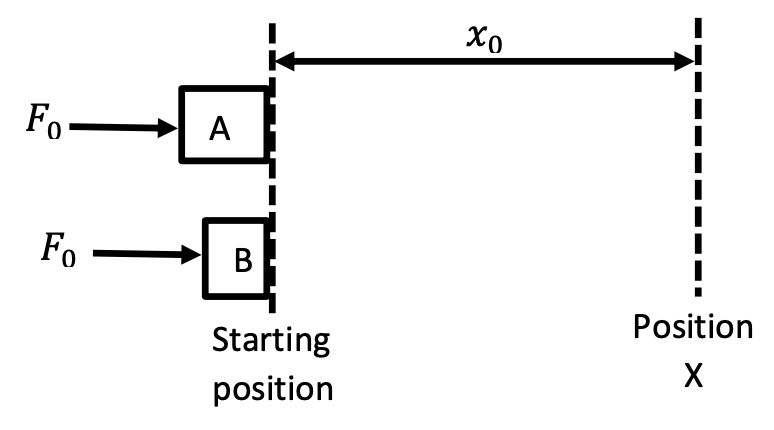
\includegraphics[width=1.0\linewidth]{images/sjpo2016q6.png}
\end{wrapfigure}
\begin{itemize}
\item[] (A) $E_A<E_B, p_A<p_B$
\item[] (B) $E_A<E_B, p_A=p_B$
\item[] (C) $E_A>E_B, p_A<p_B$
\item[] (D) $E_A=E_B, p_A=p_B$
\item[] (E) $E_A=E_B, p_A>p_B$
\end{itemize}
}
Ans: \ifpaper E \fi

\newpage \clearpage
\subsubsection{SJPO 2016 General Round Q12}
The upper end of a rope is fixed to a vertical wall. The upper end makes an angle of 30 degrees with the wall when the lower end is pulled by a horizontal force of $20 \mathrm{~N}$. What is the mass of the rope? \\
{
\begin{wrapfigure}{r}{0.5\textwidth}
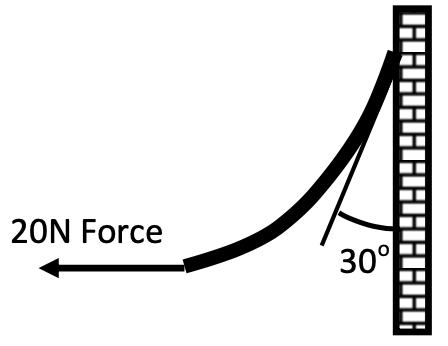
\includegraphics[width=1.0\linewidth]{images/sjpo2016q12.png}
\end{wrapfigure}
\begin{itemize}
\item[] (A) $1.8 \mathrm{~kg}$
\item[] (B) $2.0 \mathrm{~kg}$
\item[] (C) $2.4 \mathrm{~kg}$
\item[] (D) $3.5 \mathrm{~kg}$
\item[] (E) $4.1 \mathrm{~kg}$
\end{itemize}
}
Ans: \ifpaper D \fi

\subsubsection{SJPO 2018 General Round Q11}
% SJPO 2018 General Round Q11 B
The minimum time $T$ for a car to safely overtake a long trailer is measured from the time the front of the car is level with the rear of the trailer, until the rear of the car is one full car-length ahead of the trailer. The car is $3.5 \mathrm{~m}$ long and the trailer is $15.0 \mathrm{~m}$ long.\\[10pt]
The graph shows the speed-time graphs of the car and the trailer. What is the minimum time $T$ ?\\
{
\begin{wrapfigure}{r}{0.5\textwidth}
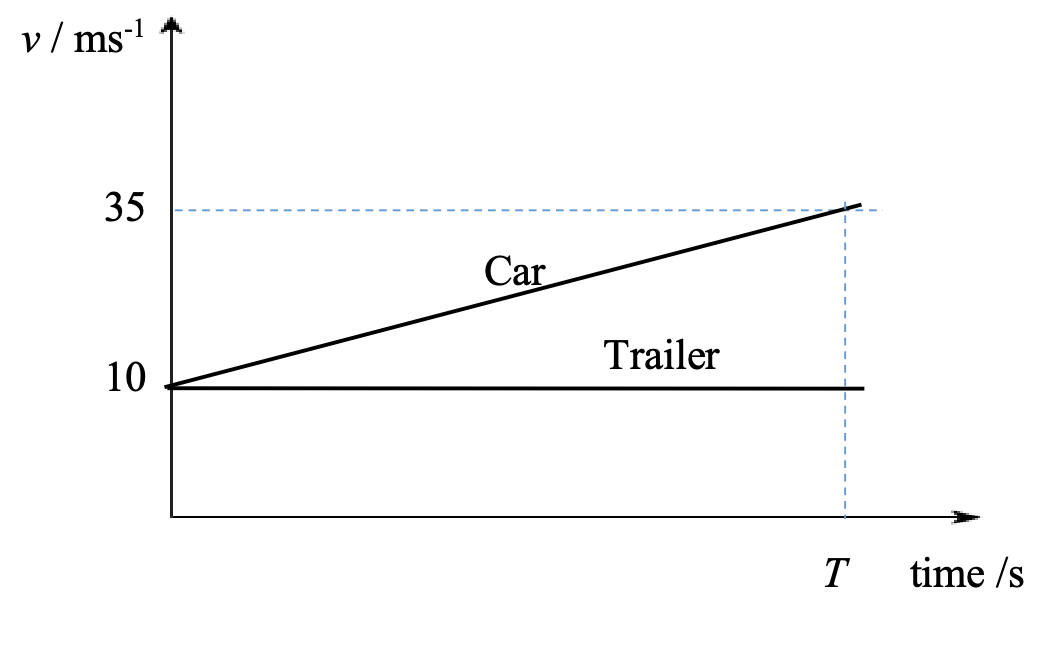
\includegraphics[width=1.0\linewidth]{images/sjpo2018q11.png}
\end{wrapfigure}
\begin{itemize}
\item[] (A) $\quad 2.16 \mathrm{~s}$
\item[] (B) $\quad 1.76 \mathrm{~s}$
\item[] (C) $\quad 1.48 \mathrm{~s}$
\item[] (D) $\quad 0.88 \mathrm{~s}$
\item[] (E) $\quad 0.64 \mathrm{~s}$
\end{itemize}
Ans: \ifpaper B \fi
}
\newpage \clearpage
\subsubsection{SJPO 2018 General Round Q12}
\label{sec:sjpo2018q12sec_static}
{
\begin{wrapfigure}{r}{0.4\textwidth}
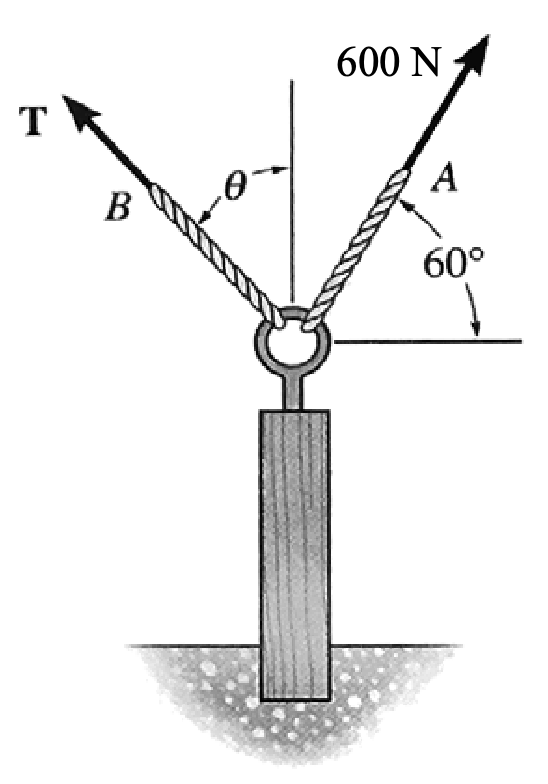
\includegraphics[width=1.0\linewidth]{images/sjpo2018q12.png}
\end{wrapfigure}
A wooden peg is to be pulled out of the ground using two ropes A and B. Rope $\mathrm{A}$ is subject to a force of $600 \mathrm{~N}$ at $60^{\circ}$ to the horizontal. Rope $\mathrm{B}$ is pulled at a fixed angle $\theta$ to the vertical. If the resultant force acting on the post is to be $1600 \mathrm{~N}$ vertically, what should be the force $T$ on rope B?
\begin{itemize}
\item[] (A) $1121 \mathrm{~N}$
\item[] (B) $1334 \mathrm{~N}$
\item[] (C) $1400 \mathrm{~N}$
\item[] (D) $1924 \mathrm{~N}$
\item[] (E) $2040 \mathrm{~N}$
\end{itemize}
Ans: \ifpaper A \fi
}

\subsubsection{SJPO 2018 General Round Q13}
Travelling with an initial speed of $70 \mathrm{~km} / \mathrm{h}$, a car accelerates at $6000 \mathrm{~km} / \mathrm{h}^2$ along a straight road. How long will it take to reach a speed of $120 \mathrm{~km} / \mathrm{h}$ ?
\begin{itemize}
\item[] (A) $30 \mathrm{~s}$
\item[] (B) $45 \mathrm{~s}$
\item[] (C) $60 \mathrm{~s}$
\item[] (D) $70 \mathrm{~s}$
\item[] (E) $180 \mathrm{~s}$
\end{itemize}
Ans: \ifpaper A \fi

\begin{samepage}
\newpage \clearpage
\subsubsection{SJPO 2018 General Round Q18}
A $2 \mathrm{~kg}$ block slides down a smooth roof which is angled at $30^{\circ}$ to the horizontal. When it reaches $\mathrm{A}$, it has a speed of $2.0 \mathrm{~m} / \mathrm{s}$. It leaves the surface of the roof at $\mathrm{B}$ and strikes the ground at a distance $d$ from the wall of the building. What is the distance $d$ ? \\
{
 \begin{wrapfigure}{r}{0.4\textwidth} 
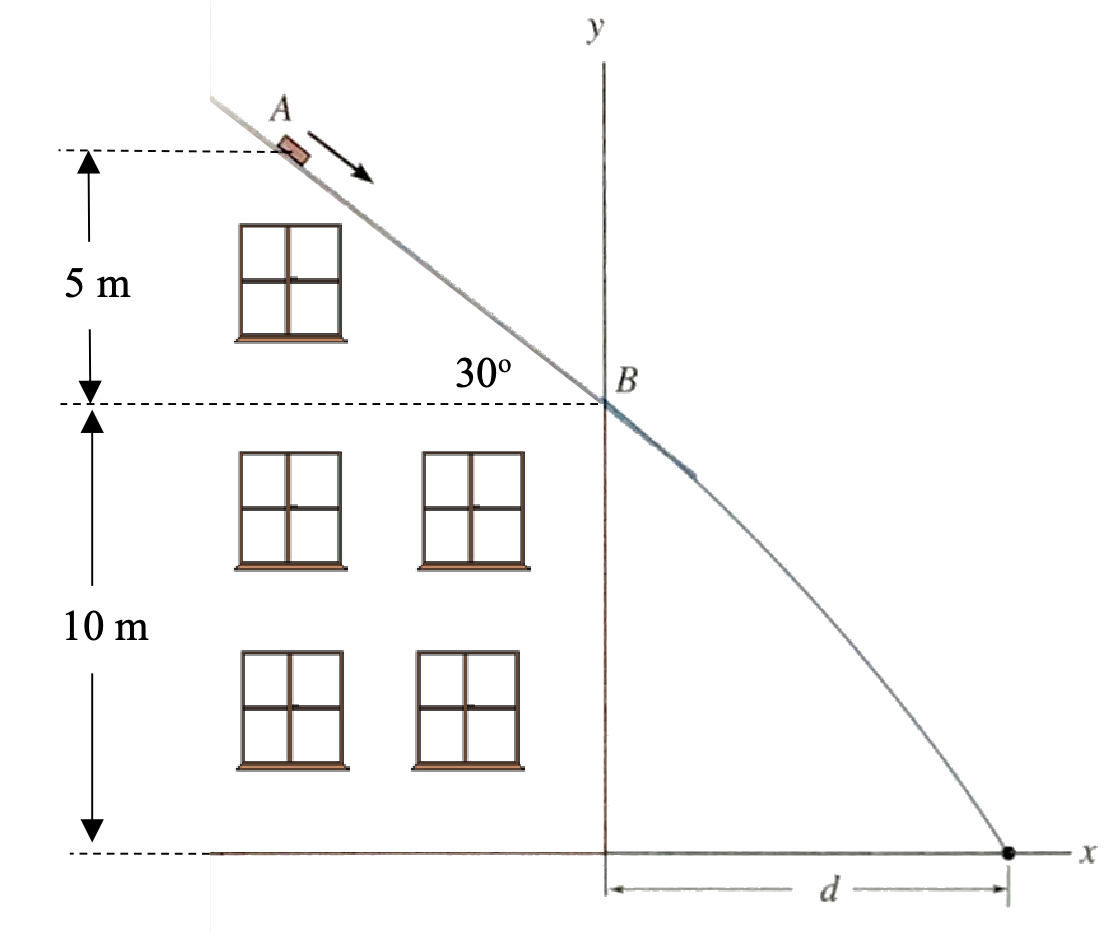
\includegraphics[width=\linewidth]{images/2018q18.png}
\end{wrapfigure}
\begin{itemize}
\item[](A) $3.96 \mathrm{~m}$
\item[](B) $8.66 \mathrm{~m}$
\item[](C) $8.78 \mathrm{~m}$
\item[](D) $17.3 \mathrm{~m}$
\item[](E) $17.8 \mathrm{~m}$
\end{itemize}
}
Ans: \ifpaper C \fi \\[10pt]
\end{samepage}



\section{Physics: Work and Impulse Topical Practice}
Read section \ref{sec:momimp} for an explanation of Work and Impulse.

\subsubsection{SJPO 2016 General Round Q5}
\url{https://youtu.be/BVb7U9s4s6s}
A train of mass $7.0 \times 10^4 \mathrm{~kg}$ expends $60 \mathrm{~kW}$ of power to travel down a $2^{\circ}$ incline at a constant velocity of $10 \mathrm{~m} \mathrm{~s}^{-1}$. How much power is required for the same train to travel up the $2^{\circ}$ incline at the same constant velocity of $10 \mathrm{~m} \mathrm{~s}^{-1}$ ?
\begin{itemize}
\item[] (A) $540 \mathrm{~kW}$
\item[] (B) $480 \mathrm{~kW}$
\item[] (C) $300 \mathrm{~kW}$
\item[] (D) $240 \mathrm{~kW}$
\item[] (E) $60 \mathrm{~kW}$
\end{itemize}
Ans:  \ifpaper A \fi

\subsubsection{SJPO 2014 General Round Q42}
A uniform chain of length $L$ and mass $m$ is lying on a smooth table. One third of its length is hanging vertically down over the edge of the table and the remaining two third is on the table. If $g$ is the acceleration due to gravity, what is the work $W$ required to pull the hanging part onto the table?
\begin{itemize}
\item[] (A) $m g L$
\item[] (B) $m g L / 3$
\item[] (C) $m g L / 6$
\item[] (D) $m g L / 9$
\item[] (E) $m g L / 18$
\end{itemize}
Ans: \ifpaper E \fi

\newpage \clearpage
\section{Math: Differential Equations}
When we studied $F(t)=ma(t)$, we noted that as long as we know the function $F(t)$, we can find $a(t)$ and integrate twice to obtain $x(t)$. However, in most systems, $F(t)$ depends on $x(t)$ or $v(t) \equiv \dot{x}(t)$. Examples include 
\begin{itemize}
    \item Spring Mass $F(x(t)) = -kx(t)$
    \item Gravitation $F(\vec{r}(t)) = -\frac{GMm}{|\vec{r}(t)|^2} \hat{r}$
    \item Drag $F(v(t)) = \frac{1}{2} \rho v(t)^2 C_D A$
    \item Lorentz Force $\vec{F} = q(\vec{E} + \vec{v} \times \vec{B})$
\end{itemize}
In these scenarios, we can no longer simply "integrate twice" since we hit a circular dependency. To resolve this, we need to solve the "differential equation". Differential equations are very common in physics. If you solve the Navier-Stokes Differential Equation, you earn a million dollars.

\subsection{What is a Differential Equation?}
When we first learned the quadratic equation, we were looking for \textbf{values} of $x$ that satisfy $$ax^2 + bx + c = 0$$  We can find 2 complex \textbf{solutions} to this \textbf{algebraic} equation
$$x = \frac{-b - \sqrt{b^2 - 4ac}}{2a} \quad \text{or}\quad x = \frac{-b + \sqrt{b^2 - 4ac}}{2a}$$
In \textbf{differential} equations, we are looking for \textbf{functions} $y(x)$ that satisfy (for example)
$$\frac{dy}{dx} = y$$
In this example, $y(x) = e^x$ works! Substitute it into the above to check that $\text{LHS} = \text{RHS}$. In fact, one can check that any multiple of $e^x$ works too! So $y(x) = A e^x$ for any arbitrary constant $A$ is a solution. To determine $A$, we need to know the "initial condition" $y(0) = A$.
\\[10pt]
Let's try another example, find the function $y(x)$ that satisfies 
$$\frac{dy}{dx} = 5y$$ with initial condition $\left. \frac{dy}{dx} \right|_{x=0} = 10$\\
Solution: $y(x) = 2e^{5x}$
\subsubsection{Physics: RC circuit} 
Find $q(t)$ that satisfies the following ($R,C$ are constants).
$$\frac{dq}{dt} = -\frac{q}{RC}$$ with initial condition $q(t=0) = q_0$. \\Answer: $q(t) = q_0 \exp (-t/RC)$ \\[10pt]
What if the initial condition was $I(t=0) := \left. \frac{dq}{dt} \right|_{t=0} = I_0$ instead? \\ Answer: $q(t) = {I_0 RC} \exp (-t/RC)$\\[10pt]

\subsection{Simple Harmonic Motion ODE}
In polynomial equations, the largest power $x^n$ is the degree $n$ of the polynomial. In differential equations, the highest derivative $\frac{d^n y}{dx^n}$ is the order of the differential equation. In this section, we cover a very common class of 2nd order differential equations
$$\frac{d^2 y}{dx^2} = -\omega^2 y$$
which has solution
$$y(x) = A\sin(\omega x + \phi)$$
\subsubsection{Derivation by Layman Arguments}
$\sin x$ and $\cos x$ are the only (proof involves linear algebra) functions that when differentiated twice, pick up a negative sign. We can afford to put a constant $\phi$ in the parameter of $\sin$, since constants vanish when differentiated. 

\subsubsection{Derivation using Complex Exponential }
\begin{align}
    \frac{d^2 y}{ dx^2} = A y     \label{eq:shm}
\end{align}
where $-\infty < A < \infty$ is a real constant.\\[10pt]
Solution: $$y=y_0 \exp(\sqrt{A}x)$$ 
Question: What happens if $A < 0$? \\
Answer: $\sqrt{A}$ is complex! To be more precise, if $A=-\omega^2$ for a positive real number $\omega$, then 
$$y=y_0 \exp(\pm i \omega x)$$
are 2 valid solutions.\\[10pt]
\textbf{A word on linear differential equation: } Equation \ref{eq:shm} is said to be linear, because if I have 2 solutions $f(x)$ and $g(x)$, then adding them together or scaling them is still a valid solution.
\begin{align}
    \text{Given } \frac{d^2 f}{ dx^2} &= A f(x)\\
    \text{And } \frac{d^2 g}{ dx^2} &= A g(x) \\
    y(x) &= f(x) + g(x)\text{ is a solution too }\\
    \text{Goal: Show } \frac{d^2y}{dx^2} & = Ay(x)\\
    \text{Proof: LHS} &= \frac{d^2}{dx^2} [f(x)+g(x)] \\
    &= \frac{d^2 f}{dx^2} + \frac{d^2 g}{dx^2} \\ 
    &= A f(x) + A g(x) \\
    &= A [f(x) + g(x)] \\
    &= \text{RHS}
\end{align}
Examples of Linear Differential Equations:
\begin{itemize}
    \item Simple Harmonic Motion
    \item RLC Circuits (linear components)
    \item (Linear) Wave Equation
    \item Schrodinger equation (Quantum Mechanics)
    \item Maxwell's Equation (Electromagnetism)
\end{itemize}
\leavevmode \\
Since $$y_+(x)=y_0 \exp(+ i \omega x)$$  $$y_-(x) = y_0 \exp(- i \omega x)$$ are 2 solutions to the \textbf{linear} DE $$\frac{d^2 f}{ dx^2} = A f(x)$$
any linear combination of them is a valid solution.

$$y(x) = C \exp(+i\omega x) + D \exp(-i \omega x)$$
where $C,D$ are arbitrary complex constants.\\[10pt]
\textbf{But what is a complex exponential? } Euler's formula: 
$$e^{i\theta} = \cos \theta + i \sin \theta$$
Some say it's just a mathematical trick, since "our system doesn't involve complex numbers". It gets philosophical. Richard Feynman famously said: "Shut up and calculate". \\[10pt]
So we want our solution $y(x)$ to be real, i.e. $\text{Im }[y(x)] = 0$. So that necessitates that $C^* = D$ and so the general solution is 
\begin{align}
    y(x) &= C \exp(+i\omega x) + C^* \exp(-i\omega x)\\
    &\quad \quad \text{By Polar Form: }C := |C| \exp(i \phi) \\
    &= |C| \text{Re}[\exp(+i (\omega x + \phi))] \\
    &= |C| \cos (\omega x + \phi)
\end{align}
which is the general solution we heuristically arrived at previously. \\[10pt]
Extra: How do we know there are no other functions that solve the ODE? The answer is we can factorise $\left(\frac{d^2}{dx^2} + \omega^2\right) = \left(\frac{d}{dx} - i\omega\right) \left(\frac{d}{dx} + i\omega\right)$ and calculate the kernel of these 2 differential operators.

\subsection{Separable ODE}
A first order separable differential equation is one of the form 
$$\frac{dy}{dx} = \frac{f(x)}{g(y)}$$
One can solve these type of equations in general by rearranging and integrating.
\begin{align}
    g(y)\ dy &= f(x)\ dx     \\
    \int g(y)\ dy &= \int f(x)\ dx
\end{align}

\subsection{1st Order ODE}
A 1st Order ODE takes the following general form
$$\frac{dy}{dx} + P(x) y = Q(x)$$
The solution is 
$$y(x) = \frac{\int \left( \exp(\int P(x)\ dx) \right) Q(x)\ dx}{ \exp(\int P(x)\ dx)}$$
Derivation: We first multiply both sides by a specific function $\mu(x)$ called the \textbf{integrating factor}, which we currently don't know the expression for.
$$\frac{dy}{dx} \mu(x) + [\mu(x) P(x)] y = \mu(x) Q(x)$$
The idea is that we want to make use of the product rule 
\begin{align}
\frac{d}{dx} [y(x) f(x)] &= \frac{dy}{dx} f(x) + \frac{df}{dx} y(x)\\
\text{which we compare with LHS}& \quad \  \frac{dy}{dx} \mu(x) + [\mu(x)P(x)]y
\end{align}
to rewrite the LHS as a total derivative. So we need to choose $\mu(x)$ to satisfy 
\begin{align}
    \mu(x) &= f(x) \\
    \mu(x) P(x) &= \frac{df}{dx}
\end{align}
This is separable, so it's just
\begin{align}
    \frac{d\mu(x)}{dx} &= \mu(x) P(x) \\
    \frac{1}{\mu(x)}\ d\mu(x) &= P(x)\ dx \\
    \int \frac{1}{\mu(x)}\ d\mu(x) &= \int P(x)\ dx \\
    \ln |\mu(x)| &= \int P(x)\ dx + C\\
    \mu(x) &= \pm e^C e^{\int P(x) \ dx}
\end{align}
After that, we substitute $\mu(x)$ back into the ODE and integrate both sides to solve for $y(x)$
\begin{align}
    \frac{d}{dx} [y(x) \mu(x)] &= \mu(x) Q(x)\\
    y(x) \mu(x) &= \int \mu(x) Q(x)\ dx\\
    y(x) &= \frac{\int \left( \exp(\int P(x)\ dx) \right) Q(x)\ dx}{ \exp(\int P(x)\ dx)}
\end{align}
Side Note: The constant of integration that appears in the integrating factor $\exp(\int P(x)\ dx)$ will cancel out. This makes sense because scaling integrating factor $\mu(x)$ by a constant $\mu(x) \mapsto \lambda \mu(x), \lambda \in \mathbb R$ shouldn't affect the solution $y(x)$ since the integrating factor was not in the original ODE.



\section{Physics: Simple Harmonic Motion (Part I)}
There are a lot of ways Simple Harmonic Motion (SHM) can appear, but one thing that is universal is that the equations of motion always simplify (usually after some approximations) to the form 
\begin{align}
    \frac{d^2 y}{dt^2} &= -\omega^2 y(t) \\
    y(t) &= A \sin (\omega t + \phi)
\end{align}
where $\omega = 2\pi/T$ will turn out to be the angular frequency of the oscillation, $T$ being the period of oscillation. \\[10pt]
Side note: The $\phi$ accounts for the $\cos$ solution by R-formula $a \sin \theta + b \cos \theta = \sqrt{a^2 + b^2} \sin(\theta + \arctan \left(\frac{b}{a}\right))$


\subsection{Spring Mass}
A mass $m$ lies on a frictionless table, attached to an unstretched spring with spring constant $k$. The other end of the spring is fixed to a wall. The mass is displaced from it's equilibrium position by $x_0$ (in a direction perpendicular to the wall) and released. Find the amplitude and period of oscillation.\\[10pt]
Hooke's Law: The restoring force $F$ of a spring stretched by $x$ is $\vec{F}(x) = -kx\ \hat{x}$.\\[10pt]
Extra: Find the period of oscillation of a mass $m$ hung vertically on a spring with spring constant $k$ in a gravitational field strength $g$.

\subsection{Spring Mass (with a Push)}
Same as the above, mass $m$ on frictioness table attached to spring with spring constant $k$ displaced by $x_0$. But this time, instead of a release, it is pushed, giving the mass an initial speed $v_0$ (toward the point of equilibrium). Find the new amplitude of oscillation.\\[10pt]
This question emphasizes the initial conditions of a differential equation.\\[10pt]
Extra: What happens if the initial speed $v_0$ was directed away from the point of equilibrium instead? Why do we get the same answer for amplitude? 


\subsection{General Pattern for SHM Questions}
I will compile all the SHM questions later on because SHM spans across all the physics topics (from EM to buoyancy), but in general the pattern is just 
\begin{itemize}
    \item[] 1. Equations of Motion (EOM)
    \item[] 2. Solve for equilibrium
    \item[] 3. Taylor expand about equilibrium
    \item[] 4. Match with the SHM equation $\ddot q(t) = -\omega^2 q(t)$
\end{itemize}
\section{Math: Polar Coordinates (2D)}
\label{sec:polar}
We previously described the location of a particle using 2 coordinates $x(t),y(t)$. When it comes to rotational questions, it's often more convenient to describe location using polar coordinates $r(t), \theta(t)$. The conversion between the coordinates are given by
\begin{align}
    r &= \sqrt{x^2 + y^2} \\
    \theta &= \operatorname{atan2} (y,x) \\ 
    x &= r \cos \theta \\
    y &= r \sin \theta
\end{align}
where $\operatorname{atan2}$ is basically $\arctan (y/x)$ but sensitive to signs.
\begin{align}
    \operatorname{atan2} (y, x)= \begin{cases}\arctan \left(\frac{y}{x}\right) & \text { if } x>0 \\ \arctan \left(\frac{y}{x}\right)+\pi & \text { if } x<0 \text { and } y \geq 0 \\ \arctan \left(\frac{y}{x}\right)-\pi & \text { if } x<0 \text { and } y<0 \\ \frac{\pi}{2} & \text { if } x=0 \text { and } y>0 \\ -\frac{\pi}{2} & \text { if } x=0 \text { and } y<0 \\ \text {undefined } & \text { if } x=0 \text { and } y=0 \end{cases} \label{eq:atan2}
\end{align}
Side Note: If we used $\theta = \arctan(y/x)$ instead, one might be worried it is unable to distinguish $(x,y)$ and $(-x,-y)$, since both result in the same numerical value for $\theta$. This is a valid mathematical concern. However, for most physics calculations we won't run into issues since we mainly deal with differential forms $ds^2 = dr^2 + r^2 d\theta^2$ and vectors (which are secretly derivatives $\partial/\partial r, \partial/\partial \theta$), both of which are "local objects". Even though the definition uses $\operatorname{atan2}(y,x)$, when performing calculations, we often pretend it is $\arctan(y/x)$ because it results in the same formulas. The reason that it gives the same results is intuitive from the definition (\ref{eq:atan2}), but to be mathematically rigorous, the proof will be annoyingly lengthy.

\subsection{Basis Vectors}
\label{sec:polarbasis}
\begin{wrapfigure}{r}{0.35\textwidth}
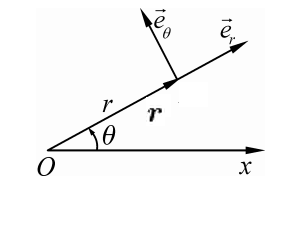
\includegraphics[width=0.9\linewidth]{images/polarbasis.png}
\caption{Basis vectors for polar coordinates}
\label{fig:polarbasis}
\end{wrapfigure}
The basis vectors for polar coordinates are shown in Figure \ref{fig:polarbasis}. To understand why they are defined as such, we should understand the motivation for defining basis vectors and vectors. The motivation is to define velocity. The essence of velocity is to know how an object's coordinates changes after a small amount of time. If a vector is $\vec{v} = 4\hat{e}_x + 3 \hat{e}_y$, it means that after a small amount of time $\Delta t$, the $x$ coordinate changes by $4 \Delta t$, and the $y$ coordinate changes by $3 \Delta t$. This implies that the direction a basis vector (e.g. $\hat{e}_x$) points, is by definition, the direction that the location moves when the coordinate (e.g. $x$) changes.\\[10pt]
For the cartesian coordinate system, the basis vectors are constant: they point in the same direction wherever we are in space. However, the basis vectors for polar coordinates are \textit{not} constant: they point in different directions depending on where we are in space. This is consequential because it implies that the derivative of the basis vectors are not zero, and this mathematical fact gives rise to fictitious/inertial forces such as centrifugal and Coriolis force!\\[10pt]
Enough talking, the expression for basis vectors 
\begin{align}
    \hat{e}_r &=\quad \cos\theta\ \hat{e}_x + \sin\theta\ \hat{e}_y \\
    \hat{e}_\theta &= -\sin\theta\ \hat{e}_x + \cos\theta\ \hat{e}_y
\end{align}
% \begin{samepage}
\subsection{Velocity in Polar Coordinates}
The velocity vector can be decomposed into the basis vectors as follows
\begin{align}
    \vec{v} = \dot{r}\ \hat{e}_r + r \dot{\theta}\ \hat{e}_\theta
\end{align}
Proof:
\begin{align}
    \vec{v} &= \frac{d\vec{r}}{dt} \\
    &= \frac{d}{dt} \left(\begin{array}{l}
         x(t) \\
         y(t) 
    \end{array}\right) \\
    &= \frac{d}{dt} \left(\begin{array}{l}
         r(t) \cos \theta(t) \\
         r(t) \sin \theta(t)
    \end{array}\right) \\
    &= \left(\begin{array}{l}
         \dot{r} \cos\theta - r\sin\theta\ \dot\theta \\
         \dot{r} \sin\theta + r\cos\theta\ \dot\theta
    \end{array}\right) \\
    &= \dot{r} \left(\begin{array}{l}
         \cos\theta \\
         \sin\theta
    \end{array}\right) + r \dot{\theta} \left(\begin{array}{l}
         -\sin\theta \\
         \ \cos\theta
    \end{array}\right) \\
    \vec{v} &= \dot{r}\ \hat{e}_r + r \dot{\theta}\ \hat{e}_\theta \label{eq:vpolar}
\end{align}
There are other ways to prove the above, but the above is simplest. 
% \end{samepage}
% \begin{samepage}
\subsubsection{SJPO 2015 General Round Q4}
Gears A, B, C are aligned side by side in such a way that rotating gear A causes gear $\mathrm{B}$ to rotate which in turn causes gear $\mathrm{C}$ to rotate. Gear A has 40 teeth and is rotating at angular speed of $50 \mathrm{rev} / \mathrm{s}$. The radius of gear B is $20 \%$ of gear $\mathrm{C}$ and gear $\mathrm{C}$ is rotating at $40 \%$ angular speed of gear $\mathrm{A}$. All the gears have the same tooth and groove size. How many teeth does gear B have?
\begin{itemize}
\item[] (A) 10
\item[] (B) 20
\item[] (C) 40
\item[] (D) 50
\item[] (E) 80
\end{itemize}
Ans: \ifpaper B \fi
% \end{samepage}
\subsection{Acceleration in Polar Coordinates}
Acceleration is the derivative of velocity (Eq \ref{eq:vpolar}) wrt time, which can be shown to be equal to 
\begin{align}
    \vec{a} = (\ddot{r} - r{\dot\theta}^2)\ \hat{e}_r + (r\ddot\theta + 2\dot r \dot \theta)\ \hat{e}_\theta
\end{align}
When we talk about \textbf{rotating reference frames} in future, the $r{\dot\theta}^2$ term is responsible for \textbf{centrifugal force}, and the $2\dot r \dot \theta$ term is responsible for \textbf{Coriolis force}. \\[10pt]
Proof: First we obtain the derivative of the polar basis vectors.
\begin{align}
    \frac{d\hat{e}_r}{dt} &= \frac{d}{dt}\left(\begin{array}{l}
         \cos\theta \\
         \sin\theta
    \end{array}\right) \\ 
    &= \left(\begin{array}{l}
         -\sin\theta \ \dot\theta  \\
         \ \cos\theta \ \dot\theta 
    \end{array}\right)\\
    &= \dot\theta\ \hat{e}_\theta \\
    \frac{d\hat{e}_\theta}{dt} &= \frac{d}{dt}\left(\begin{array}{l}
         -\sin\theta \\
         \ \cos\theta
    \end{array}\right) \\ 
    &= \left(\begin{array}{l}
         -\cos\theta \ \dot\theta  \\
         - \sin\theta \ \dot\theta 
    \end{array}\right)\\
    &= -\dot\theta\ \hat{e}_r 
    \end{align}
Then we simply apply chain rule
    \begin{align}
    \vec{a} &= \frac{d\vec{v}}{dt} \\
    &= \frac{d}{dt} (\dot{r}\ \hat{e}_r + r \dot{\theta}\ \hat{e}_\theta )\\
    &= \ddot{r}\ \hat{e}_r + \dot{r} \frac{d\hat{e}_r}{dt} + \dot r\dot\theta \ \hat{e}_\theta + r \ddot \theta \ \hat{e}_\theta + r\dot\theta \frac{d\hat{e}_\theta}{dt} \\
    &= (\ddot{r} - r{\dot\theta}^2)\ \hat{e}_r + (r\ddot\theta + 2\dot r \dot \theta)\ \hat{e}_\theta
\end{align}

\section{Physics: Centripetal Force and Acceleration}
Newton's 2nd law is just
\begin{align}
    F_r\ \hat{e}_r + F_\theta\ \hat{e}_\theta = \vec{F}_{net} & = m \vec{a} = m \left[(\ddot{r} - r{\dot\theta}^2)\ \hat{e}_r + (r\ddot\theta + 2\dot r \dot \theta)\ \hat{e}_\theta \right]\\
    \Rightarrow F_r &= m(\ddot r - r{\dot\theta}^2) \\ 
    \text{and } F_\theta &= m (r\ddot\theta + 2 \dot r \dot \theta)  
\end{align}
\subsection{Centripetal Acceleration}
\url{https://youtu.be/_noiaP-pKmU}\\
Often, the radial coordinate function $r(t)$ is constant. Examples include: pendulum, point mass sliding down hemisphere, planet in orbit, cup on rotating Chinese table. When $\dot r = 0$, Newton's 2nd law simplifies to
\begin{align}
    F_r &= -mr {\dot\theta}^2 \\
    F_\theta &= mr\ddot\theta
\end{align}
\subsubsection{SJPO 2015 General Round Q1}
\url{https://youtu.be/WG41FvYPYkQ}\\
Two identical masses, $\mathrm{A}$ and $\mathrm{B}$, are tied to strings and placed on a horizontal frictionless disc as in the figure below. The two masses are then set to move about the centre of the disc with the same angular velocity $\omega$. Given that the tension of the string connecting mass $\mathrm{A}$ to the center of the disc is $T$, determine the tension of the string connecting mass $\mathrm{B}$ to mass $\mathrm{A}$. \\
{
\begin{wrapfigure}{r}{0.5\textwidth}
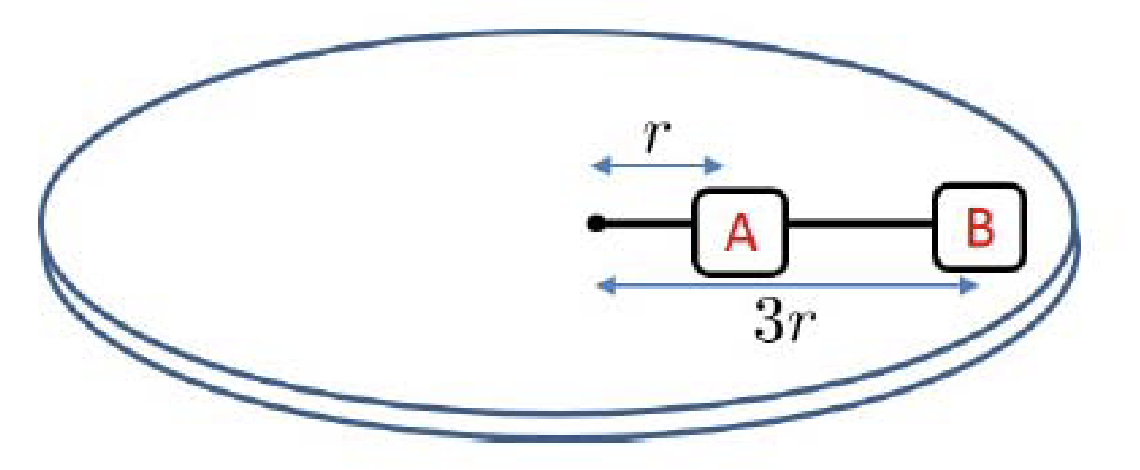
\includegraphics[width=1.0\linewidth]{images/sjpo2015q1.png}
\end{wrapfigure}
\begin{itemize}
\item[] (A) $T / 4$
\item[] (B) $3 T / 4$
\item[] (C) $T$
\item[] (D) $3 T$
\item[] (E) $4 T$
\end{itemize}
}
Ans: \ifpaper B \fi
\subsubsection{SJPO 2018 General Round Q7}
\url{https://youtu.be/V-DVhjbQa5o}\\
A bug is just about to slip on a circular turntable of radius $R$ rotating at constant angular velocity. The bug is halfway between the centre and the edge and the coefficient of static friction is $1 / 4$. What is the acceleration of the bug?
\begin{itemize}
\item[] (A) $3 g$
\item[] (B) $2 g$
\item[] (C) $3 g / 2$
\item[] (D) $g / 2$
\item[] (E) $g / 4$
\end{itemize}
Ans: \ifpaper E \fi

\subsubsection{SJPO 2016 General Round Q14 \& Q15}
\url{https://youtu.be/VI1WY_f8QL0}\\
\textbf{Q14}: A ball with mass $m$ is hung from the ceiling with a massless string of length $l$ as shown in the diagram. It moves in uniform circular motion with angular velocity $\omega$. What is the magnitude of tension in the string? \\
{
\begin{wrapfigure}{r}{0.5\textwidth}
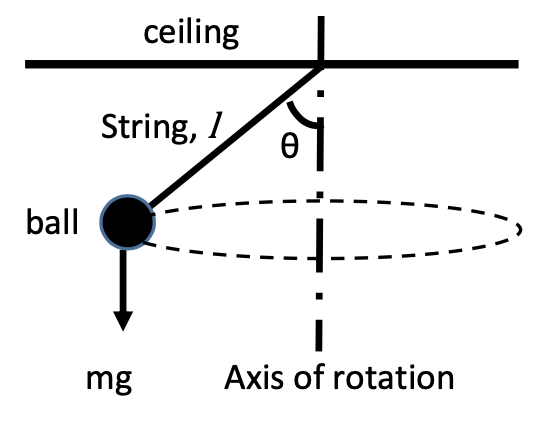
\includegraphics[width=1.0\linewidth]{images/sjpo2016q14.png}
\end{wrapfigure}
\begin{itemize}
\item[] (A) $m \omega^2 l$
\item[] (B) $m \omega^2 l \cos \theta$
\item[] (C) $m \omega^2 l / \cos \theta$
\item[] (D) $m \omega^2 l \sin \theta$
\item[] (E) $m \omega^2 l / \sin \theta$
\end{itemize}
}
Ans: \ifpaper A \fi\\[30pt]
\textbf{Q15}: \url{https://youtu.be/j_T73abVdBs} \\
For the same situation as in the above question, with $m=0.20 \mathrm{~kg}, l=0.80 \mathrm{~m}$. What is the angular velocity in order for the string to maintain a constant angle of $\theta=25^{\circ}$ to the vertical?
\begin{itemize}
\item[](A) $0.59 \mathrm{rad} \mathrm{s}^{-1}$
\item[](B) $1.2 \mathrm{rad} \mathrm{s}^{-1}$
\item[](C) $3.5 \mathrm{rad} \mathrm{s}^{-1}$
\item[](D) $3.7 \mathrm{rad} \mathrm{s}^{-1}$
\item[](E) $5.4 \mathrm{rad} \mathrm{s}^{-1}$
\end{itemize}
Ans: \ifpaper D \fi 
\newpage
\subsubsection{SJPO 2016 General Round Q17}
\url{https://youtu.be/-UeWL4MssRA}\\
A $360 \mathrm{~kg}$ roller coaster car is initially at rest at a height of $120 \mathrm{~m}$ above the ground. It goes to the ground and does a circular loop of radius $r$. Assume that friction and energy losses are negligible, the car is small and is not attached to the track. What is the maximum radius $r$ so that the roller coaster does not leave the track? \\ 
{
\begin{wrapfigure}{r}{0.6\textwidth}
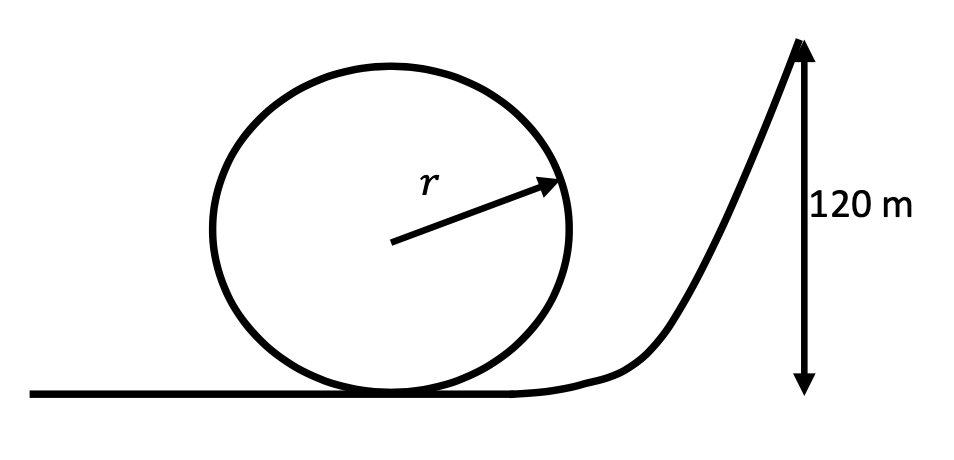
\includegraphics[width=1.0\linewidth]{images/sjpo2016q17.png}
\end{wrapfigure}
\begin{itemize}
\item[] (A) $120 \mathrm{~m}$
\item[] (B) $60 \mathrm{~m}$
\item[] (C) $48 \mathrm{~m}$
\item[] (D) $42 \mathrm{~m}$
\item[] (E) $36 \mathrm{~m}$
\end{itemize}
}
Ans: \ifpaper C \fi
\subsection{Example: Pendulum}
A mass $m$ is hung by an inextensible string of length $l$ in a gravitational field strength $g$. It is displaced by a small angular displacement $\theta_0$ and released. Find the amplitude and period of oscillation.\\[10pt]
Ans: \\[100pt]
\newpage \clearpage
\begin{samepage}
\subsubsection{SJPO 2015 General Round Q16}
As shown in the diagram, a pendulum of length $L$ is hung from the ceiling and at a point $P$, a peg is placed. $L^{\prime}$ denotes the shortened length of the pendulum during part of its oscillation. The period of the pendulums oscillation is now \\
{
\begin{wrapfigure}{r}{0.4\textwidth}
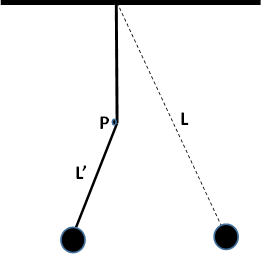
\includegraphics[width=1.0\linewidth]{images/2015q16.png}
\end{wrapfigure}
\begin{itemize}
\item[](A) $2 \pi \sqrt{\frac{L}{g}}$
\item[](B) $2 \pi \sqrt{\frac{L^{\prime}}{g}}$
\item[](C) $2 \pi\left[\sqrt{\frac{L}{g}}+\sqrt{\frac{L^{\prime}}{g}}\right]$
\item[](D) $\pi\left[\sqrt{\frac{L}{g}}+\sqrt{\frac{L^{\prime}}{g}}\right]$
\item[](E) $\pi \sqrt{\frac{L+L^{\prime}}{g}}$
\end{itemize}
}
\noindent Ans: \ifpaper D \fi
\end{samepage}

\begin{samepage}
\subsubsection{SJPO 2018 General Round Q21}
The bob of a simple pendulum travels $2 \mathrm{~m}$ in one complete oscillation in a time of $2.000 \mathrm{~s}$. Assuming that damping is negligible, when the same pendulum is made to travel $4 \mathrm{~m}$ in one complete oscillation, the time taken is
\begin{itemize}
\item[](A) $4.000 \mathrm{~s}$
\item[](B) More than $2.000 \mathrm{~s}$
\item[](C) $2.000 \mathrm{~s}$
\item[](D) Less than $2.000 \mathrm{~s}$
\item[](E) $1.000 \mathrm{~s}$
\end{itemize}
Ans: \ifpaper B \fi 
\end{samepage}

\newpage \clearpage
\section{Physics: Rotational Dynamics}
\subsection{SUVAT for Rotational Kinematics}
We know that for 1D kinematics
\begin{align}
    a = \frac{dv}{dt} = \frac{d^2 s}{dt^2}
\end{align}
leads to the SUVAT rules
\begin{align}
v(t)&=u+a t  \\
s(t)&=u t+\frac{1}{2} a t^2 \\
 v(s)^2&=u^2+2 a s  \\
 s(t)&=\frac{v(t)+u}{2} t \\
 s(t)&=v(t) t-\frac{1}{2} a t^2 
\end{align}
It hence comes as no surprise that since
\begin{align}
    \alpha = \frac{d\omega}{dt} = \frac{d^2 \theta}{dt^2}
\end{align}
we have analogous "SUVAT" rules for rotational motion
\begin{align}
\omega(t)&=\omega_0+\alpha t \\
\theta (t)&=\omega_0 t+\frac{1}{2} \alpha t^2 \\
 \omega(\theta )^2&=\omega_0^2+2 
 \alpha \theta  \\
 \theta (t)&=\frac{\omega(t)+\omega_0}{2} t \\
 \theta (t)&=\omega(t) t-\frac{1}{2} 
 \alpha t^2 
\end{align}\\[0pt]
That's cool! But what about dynamics? What is mass, force, momentum, kinetic energy, analogous to? \\[10pt]
We will now show that the analogy is as follows
\begin{center}
\begin{tabular}{ |c|c| } 
 \hline
  Translational & Rotational \\ \hline \hline
  Mass $m$ & Moment of Inertia $I$ \\ \hline
  Force $F$ & Torque $\tau$ \\ \hline
  Momentum $mv$ & Angular Momentum  $I\omega$\\\hline
  Kinetic Energy $\frac{1}{2}mv^2$ & Kinetic Energy $\frac{1}{2} I \omega^2$ \\\hline
\end{tabular}
\end{center}

\subsection{Moment of Inertia}
So far we have been dealing with point masses. But in reality most objects take up some volume. \\[10pt]
Before we talk about \textit{continuous} mass distributions, let's derive everything using discrete masses first. \\[10pt]
\underline{\textbf{One mass $m$ at radius $r$}}: \\[2pt]
Suppose there is a mass $m$ distance $r$ away from the origin, rotating about an axis passing through the origin with angular velocity $\omega$. \\[10pt]
Qn: What is its magnitude of the velocity? \\[0pt]
Ans: The magnitude of the velocity of the mass is $|\vec{v}| = r\omega$. \\[10pt]
Qn: What is the direction of the velocity? \\[0pt]
Ans: Tangential to the imaginary circle of radius $r$. \\[10pt]
Qn: What is its kinetic energy (KE)? \\[0pt]
Ans: The KE is $\frac{1}{2} m |\vec{v}|^2 = \frac{1}{2} (mr^2) \omega^2$.\\[10pt]
We expressed KE in the form of $\frac{1}{2} I \omega^2$ because this form generalises to other mass distributions. \\[10pt]
\underline{\textbf{Two masses $m/2$ at same radius $r$}}: \\[2pt] Suppose we split the $m$ into half, and put the 2 masses (each of mass $m/2$) at coordinates $(0,r)$ and $(0,-r)$. They rotate about the origin at angular velocity $\omega$. \\[10pt]
Qn: What are their velocities? \\[0pt]
Ans: Both velocities' magnitudes are $|\vec{v}_1| = |\vec{v}_2| = r\omega$. Both velocities' directions are tangent to the circle of radius $r$, but point in opposite directions. \\[10pt]
Qn: What is the total KE? \\[0pt]
Ans: The total KE is $$\frac{1}{2} \left(\frac{m}{2}\right) |\vec{v}_1|^2 + \frac{1}{2} \left(\frac{m}{2}\right) |\vec{v}_2|^2 = \frac{1}{2} \left[ \left(\frac{m}{2} \right) r^2 + \left( \frac{m}{2}\right) r^2 \right] \omega^2 $$
\underline{\textbf{Two masses $m/2$ at different radii $r,2r$}}: \\[2pt]
Suppose we have two masses, each of mass $m/2$. We place them at coordinates $(0,r)$ and $(0,2r)$. They rotate about the origin at angular velocity $\omega$.\\[10pt]
Qn: What are their velocities? \\[0pt]
Ans: For the mass at $(0,r)$, the velocity is $|\vec{v}_1| = r\omega$ in the leftward direction. For the mass at $(0,2r)$, the velocity is $|\vec{v}_2| = 2r\omega$ in the leftward direction. \\[10pt]
Qn: What is the total KE? \\[0pt]
Ans: The total KE is 
\begin{align}
\frac{1}{2} \left(\frac{m}{2}\right) |\vec{v}_1|^2 + \frac{1}{2} \left(\frac{m}{2}\right) |\vec{v}_2|^2 = \frac{1}{2} \left[ \left(\frac{m}{2} \right) r^2 + \left( \frac{m}{2}\right) (2r)^2 \right] \omega^2 \notag 
\end{align}
\underline{\textbf{General Collection of Discrete Masses}}: \\[2pt] For a general collection of masses $\{m_1,m_2,...\}$ located at distances $\{r_1, r_2, ...\}$ from the origin, as long as they are rotating about the origin with the \textbf{same angular velocity} $\omega$. We can "pre-calculate" the quantity 
\begin{align}
I = \sum_i m_i r_i^2  \label{eq:mom}    
\end{align}
and use this quantity in the calculation of kinetic energy $$K.E. = \frac{1}{2} I \omega^2 $$
We call $I$ the \textbf{Moment of Inertia}. It is used all over rotational physics, such as in the calculation of angular momentum, precession (gyroscopes). It is \textbf{analogous to mass} in translational dynamics (we will see this soon).\\[10pt]
\underline{\textbf{General Mass Distribution}}: \\[2pt] Physicists model \textbf{rigid body} objects as a uniform mass density over some volume. It is made up of many small masses $dm = \rho dV$, where $dm$ is called an infinitesimal mass element and $dV = dx\ dy\ dz$ is an infinitesimal volume element. If we integral $dm$ over volume $\mathcal{V}$ the object occupies, we get the mass
\begin{align}
    \int_{\mathcal V} dm = m
\end{align}
To find $I$ for a general mass distribution, we turn the sum into an integral in Equation \ref{eq:mom}. So we have
\begin{align}
    I = \int_{\mathcal V} r^2 dm 
\end{align}
where $r$ is the \textbf{distance} of the infinitesimal mass $dm$ \textbf{from the axis of rotation}.
\newpage \clearpage
\noindent Listed above is a list of moment of inertia of common objects. Calculating them involves 2D integrals, which we postpone to a future chapter. 
\begin{figure}[t]
    \centering
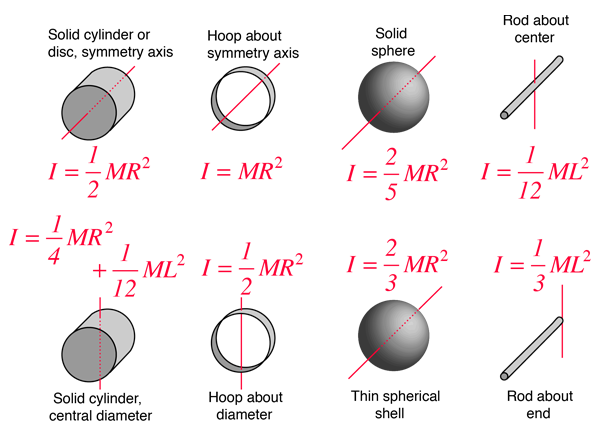
\includegraphics[width=1.0\linewidth]{images/commonmoi.png}\\
\caption{Source: Hyperphysics}
\end{figure}

\subsubsection{SJPO 2018 General Round Q9}
The moment of inertia of a solid sphere of mass $M$ and radius $a$, about an axis passing through its centre, is $(2 / 5) M a^2$. The mass of a solid uniform octant (one-eighth) of a sphere of radius $a$, is $m$. The moment of inertia about an axis along one of the straight edges (e.g. $z$ axis) is\\
\begin{wrapfigure}{r}{0.3\textwidth}
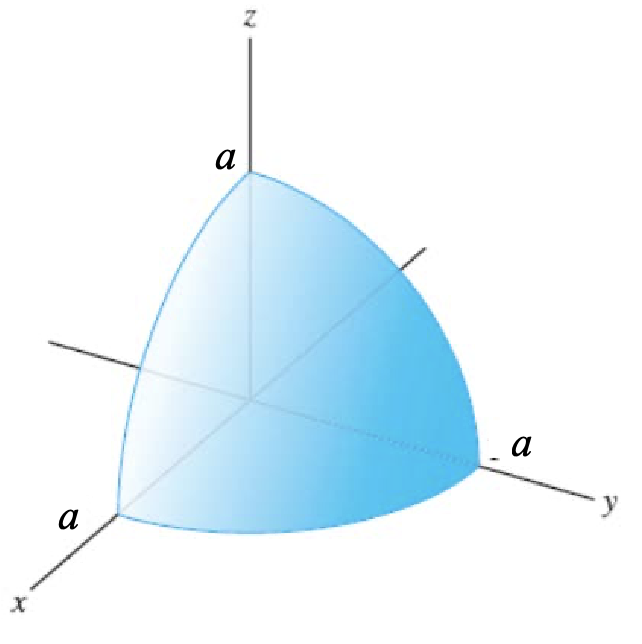
\includegraphics[width=1.0\linewidth]{images/sjpo2018q9.png}
\end{wrapfigure}
\begin{itemize}
\item[](A) $\frac{4}{3} m a^2$
\item[](B) $\frac{2}{5} m a^2$
\item[](C) $\frac{3}{8} m a^2$
\item[](D) $\frac{1}{8} m a^2$
\item[](E) $\frac{1}{20} m a^2$
\end{itemize}
Ans: \ifpaper B \fi 
\newpage \clearpage
\subsection{Angular Momentum and Torque (in 3D)}
Angular momentum $\vec{L}(t)$ of a point particle at $\vec{r}(t)$ with momentum $\vec{p}(t)$ \textbf{about the origin} is defined as 
\begin{align}
    \vec{L}(t) &\equiv \vec{r}(t) \times \vec{p}
\end{align}
Similar to how $\vec{F} = d\vec{p}/dt$, if we differentiate $\vec{L}$ wrt time, we arrive at the definition for torque $\vec{\tau}$
\begin{align}
    \vec{\tau}(t) &\equiv \frac{d\vec{L}}{dt}  \\
    &=\vec{r} \times \frac{\mathrm{d} \vec{p}}{\mathrm{d} t}+\frac{\mathrm{d} \vec{r}}{\mathrm{d} t} \times \vec{p}\\
&=\vec{r} \times \vec{F}+\vec{v} \times \vec{p}\\
&=\vec{r} \times \vec{F}\\
\end{align}
Extra: The definition of angular momentum can be motivated from Lagrangian mechanics as a conserved quantity from rotational invariance.
\subsubsection{Conceptual Emphasis}
I want to re-emphasise on some important conceptual points:
\begin{itemize}
    \item Angular velocity $\omega(t) = d\theta/dt$ is a \textbf{scalar}. It is defined about an \textbf{axis of rotation} $\mathbf{\hat{e}}_{\text{rot}}$.
    \item Torque $\vec{\tau} =\vec{r} \times \vec{F}$ is a \textbf{vector}. \\ Its value depends on our \textbf{choice of origin} (which affects the value of $\vec{r}$).
    \item Angular momentum $\vec{L} = \vec{r} \times \vec{p}$ is a \textbf{vector}. \\ Its value depends on our \textbf{choice of origin} (which affects the value of $\vec{r}$).
\end{itemize}
Extra: Sometimes (mostly used in 3D) we package $\omega \text{ \& } \mathbf{e}_{\text{rot}}$ into a single angular velocity \textbf{vector} $\vec{\omega} = \omega \mathbf{\hat{e}}_{\text{rot}}$, which makes it a vector. \\[10pt]
Extra: If the axis of rotation changing over time (such as a wheel), one can consider the instantaneous axis of rotation \url{https://en.wikipedia.org/wiki/Instant_centre_of_rotation}.
\subsubsection{Angular Momentum in terms of $I$}
For a point particle at $(r,0,0)$ rotating about z-axis with angular velocity $\omega$, 
\begin{align}
    L_z &= r p \\
    &= r mv \\
    &= r m \omega r \\ 
    &= mr^2 \omega
\end{align}
In general, for a rigid body that is rotating about one of its \textbf{principal axis of rotation} (an advanced concept you don't need to worry about now) with angular velocity $\vec{\omega}$, it's angular momentum is
\begin{align}
    \vec{L} = I \vec{\omega}
\end{align}
where $I$ (a scalar) is the moment of inertia about that axis of rotation. \\[10pt]
Extra: If the rigid body is not rotating about a principal axis of rotation, then $\vec{L} = \mathbf{I} \vec{\omega}$ where $\mathbf{I}$ is the \textbf{inertia tensor} \url{https://en.wikipedia.org/wiki/Moment_of_inertia#Inertia_tensor}
\newpage
\subsection{Angular Momentum and Torque (in 2D)}
\label{sec:torque}
The exact "vector nature" of $\vec{L},\vec{\tau},\vec{\omega}$ is quite complicated and will be discussed in future. For now we are mostly concerned with the magnitude of $\vec{L}$. Specifically, for the following section, we will only consider scenarios where torque is parallel to angular momentum, so the direction of angular momentum remains constant. So we use the same symbols without the arrow above to denote the magnitude.
\begin{align}
    L \equiv |\vec{L}| \\
    \omega \equiv |\vec{\omega}| \\
    {\tau} \equiv |\vec{\tau}|
\end{align}
In other words, for now you can forget the vector nature of these quantities and just work with the following 
\begin{align}
    L &= I\omega \\
    \tau = rF \sin \theta_{rF} &= \frac{dL}{dt} = I\alpha \\
    I \text{ can be obtained } & \text{from the list of MOIs}
\end{align}
\subsubsection{Using $r_\perp F$ vs $r F_\perp$}
There are 2 ways to visualise $\tau = rF \sin \theta_{rF}$\\[0pt]
{
\begin{wrapfigure}{r}{0.4\textwidth} 
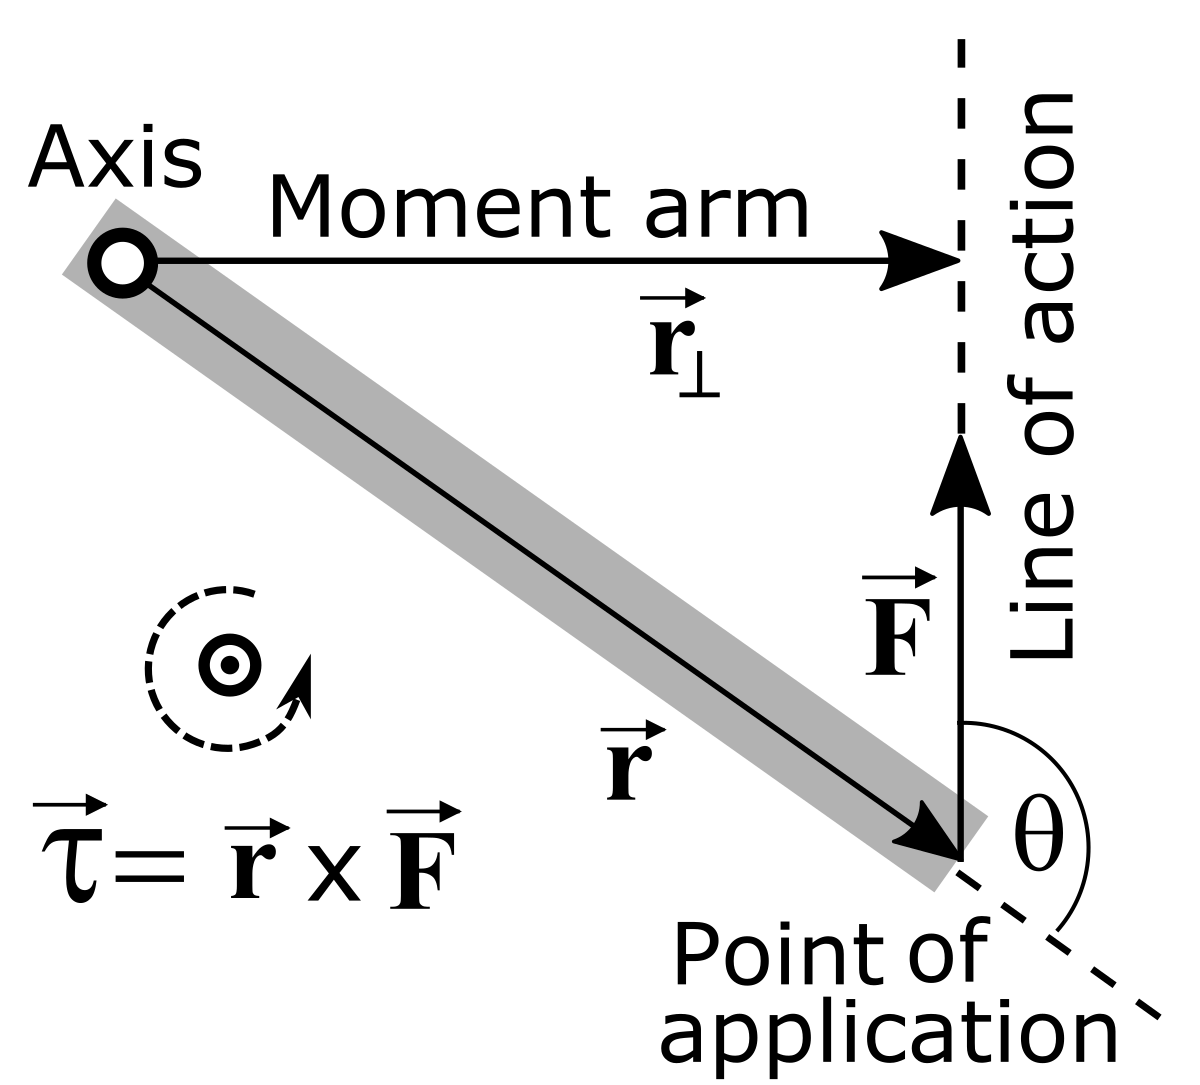
\includegraphics[width=\linewidth]{images/lineofaction.png}
\\[20pt]
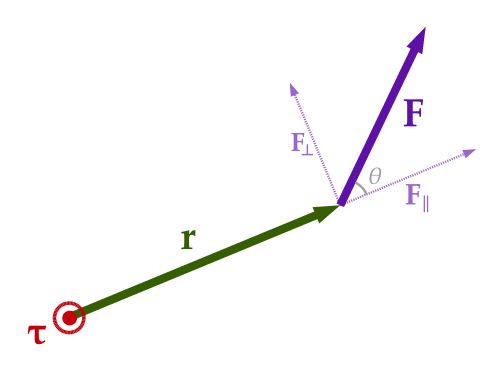
\includegraphics[width=\linewidth]{images/fperp.png}
\end{wrapfigure}
\\[20pt]Projecting the origin $O$ onto the \textbf{line of action} of the force, $r_\perp$ is the shortest distance from $O$ to the line of action.
\begin{align*}
|\vec{\tau}| & =|\vec{r} \times \vec{F}| \\
& =|r F \sin \theta_{rF}| \\
& =r_{\perp} F \\
\end{align*}\\[10pt]
Projecting the tip of the force vector onto the extended $\vec{r}$ vector (aka "$OR$ produced"), $F_\perp$ is the shortest distance from the tip to $OR$ produced.
\begin{align*}
|\vec{\tau}| & =|\vec{r} \times \vec{F}| \\
& =|r F \sin \theta_{rF}| \\
& =r F_{\perp} \\
\end{align*}
}
\clearpage
\subsubsection{Physical Intuition} 
Intuition for torque causing angular momentum to change in 2D: 
\begin{itemize}
    \item If force is at $\theta_{rF} = 90^\circ$, maximal torque in the \textbf{CCW} direction ($\vec{L}$ pointing \textbf{out} of the page).
    \item If force is at $\theta_{rF} = 0^\circ$, no torque. More on this in \ref{chap:centralforce}.
    \item If force is at $\theta_{rF} = -90^\circ$, maximal torque in the \textbf{CW} direction ($\vec{L}$ pointing \textbf{into} the page).
    \item Momentum $\vec{p}$ vs angular momentum $L_z$. Example: uniform circular motion of 1 and 2 particles in the x-y plane.
\end{itemize}
Intuition for angular momentum in 2D:
\begin{itemize}
    \item Spinning ice skater \url{https://youtu.be/FmnkQ2ytlO8}
    \item Guy spinning on chair \url{https://youtu.be/M6PuutIm5h4}
\end{itemize}
\subsubsection{Example: Oscillation of General Object}
Qn: If you pin a laminar with moment of inertia $I$ such that it can freely rotate about its pivot, and the center of mass is distance $L$ away from the pivot, show that the angular frequency of oscillations is given by $$\omega = \sqrt{\frac{mgL}{I}}$$
\subsubsection{SJPO 2016 General Round Q16}
The diagram below shows 3 pendulums of length $\mathrm{L}$. The first uses a point mass $\mathrm{m}$ suspended from a string of length $\mathrm{L}$; the second uses a sphere with radius $\mathrm{R}$ and mass $\mathrm{m}$ suspended such that the centre of mass of the sphere is length $L$ away from the pivot point; the last uses a rigid rod of length $L$ and mass $\mathrm{m}$ pivoted at its end. Which of the following statements correctly describes the periods of these 3 pendulums?\\
\noindent Hint: Moment of inertia of the 3 setups are $I_2>I_1>I_3$ \\
{
\begin{wrapfigure}{r}{0.5\textwidth} 
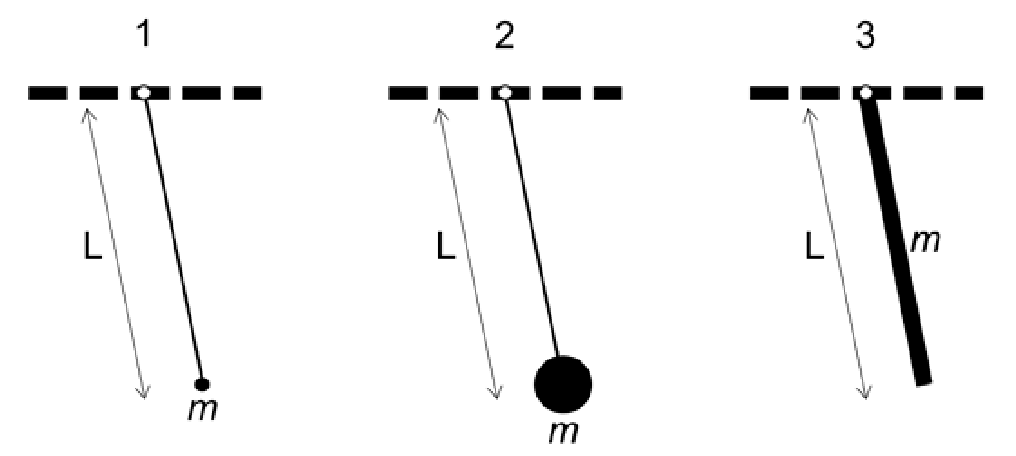
\includegraphics[width=\linewidth]{images/sjpo2016q16.png}
\end{wrapfigure}
\begin{itemize}
\item[] (A) Period of $1=2>3$
\item[] (B) Period of $2>1>3$
\item[] (C) Period of $2>3>1$
\item[] (D) Period of $3>1>2$
\item[] (E) Period of $3>2>1$
\end{itemize}
}
Ans: \ifpaper B \fi
\subsubsection{Qn: Taylor Example 3.3}
A uniform circular turntable (mass $M$, radius $R$, center $O$) is at rest in the x-y plane and is mounted on a frictionless axle, which lies along the vertical $z$ axis. I throw a lump of putty (mass $m$) with speed $v$ toward the edge of the turntable, so it approaches along a line that passes within a distance $b$ of $O$, as shown in Figure \ref{fig:taylor3.3}. When the putty hits the turntable, it sticks to the edge, and the two rotate together with angular velocity $\omega$. Find $\omega$. \\
{
\begin{wrapfigure}{r}{0.6\textwidth} 
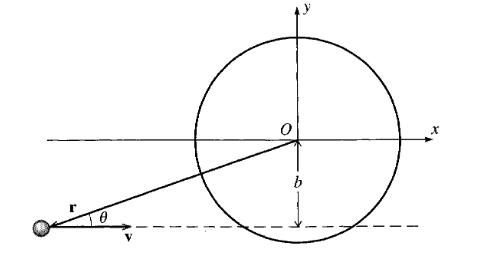
\includegraphics[width=\linewidth]{images/taylor3.3.png}
\label{fig:taylor3.3}
\caption{A lump of putty of mass $m$ is thrown with velocity $\mathbf{v}$ at a stationary turntable. The putty's line of approach passes within the distance $b$ of the table's center $O$.}
\end{wrapfigure}\\[200pt]
}
\noindent Ans: $\omega = \frac{m}{m+M/2} \frac{vb}{R^2}$\\
\noindent Extra: Can we use conservation of momentum? Why not?
\subsection{Central Forces Conserve Angular Momentum}
\label{chap:centralforce}
\subsubsection{2D Explanation}
Looking at $\tau = rF \sin \theta_{rF}$, we see that if the applied force is pointing to or away from the origin, then it doesn't cause any increased rotation (intuition). Mathematically, $\theta_{rF}=0^\circ\text{ or } 180^\circ$. For better intuition, consider a ball on a string going in constant-radius circular motion on a frictionless x-y plane. The ball maintains it's angular velocity. 
\subsubsection{3D/Vector Explanation}
Torque $\vec{\tau} = \vec{r} \times \vec{F}$ is the cross product between position $\vec{r}$ and force $\vec{F}$. If the force is parallel or anti-parallel to the position (pointing away or towards the origin), then torque is zero, since $\vec{\tau} = \vec{r} \times k\vec{r} = \vec{0}$. This means \textbf{angular momentum is conserved}, since ${d\vec{L}}/dt = \vec{\tau} = \vec{0}$.
\subsubsection{Qn: Taylor Problem 3.25}
A particle of mass $m$ is moving on a frictionless horizontal table and is attached to a massless string, whose other end passes through a hole in the table, where I am holding it. Initially the particle is moving in a circle of radius $r_0$ with angular velocity $\omega_0$, but I now \textbf{slowly} pull the string down through the hole until a length $r$ remains between the hole and the particle. What is the particle's angular velocity now?\\[10pt]
Ans: $\omega = \omega_0 (r_0/r)^2 $ \\[10pt]
Extra: Does the kinetic energy increase? Does work energy theorem apply? 


\subsection{Rotational Kinetic Energy}
As motivated previously, the kinetic energy of an object with angular velocity $\omega$ (about some axis of rotation) and moment of inertia $I$ (about the \textbf{same} axis of rotation) is $$K.E. = \frac{1}{2} I \omega^2$$

\subsubsection{Qn: Morin Problem 8.26 (Swinging stick)}
A uniform stick of length $L$ is pivoted at its bottom end and is initially held vertical. It is given an infinitesimal kick, and it swings down around the pivot. After three-quarters of a turn (in the horizontal position shown in Figure \ref{fig:morin8.26}), the pivot is somehow vaporized, and the stick flies freely up in the air. What is the angular velocity of the stock when the pivot is vaporized? 
\begin{wrapfigure}{r}{0.3\textwidth} 
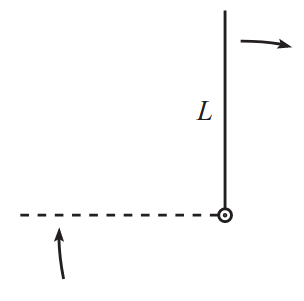
\includegraphics[width=\linewidth]{images/morin8.26.png}
\label{fig:morin8.26}
\end{wrapfigure}\\
Ans: $\omega = \sqrt{3g/L}$\\[5pt]
Extra Qn: What is the maximum height of the center of the stick in the resulting motion? At what angle is the stick tilted when the center reaches this maximum height? \\[5pt]
Ans: $3L/8, 1.5\text{ rad}$
\newpage\clearpage 
\section{Physics: Statics}
Now that we have covered friction, normal contact force, and tension (Section \ref{sec:fnt}) and Torque (Section \ref{sec:torque}), we can now learn some olympiad tricks to solve statics questions!\\[10pt]
We know already that in static equilibrium (nothing moving rotationally and translationally), net torque and net force must be 0. In general it's possible to write out all the equations. But sometimes we can use shortcuts.
\subsection{Balancing Translational Forces}
Translationally, net force must be zero. i.e. $$\sum_i F_{i,x} = \sum_i F_{i,y} = \sum_i F_{i,z} = 0$$
It will be useful to know how to solve simultaneous linear equations of 3 variables in your scientific calculator. \\[10pt]
Extra: Or know how to take the inverse of a 3x3 matrix in your graphing calculator.
\subsubsection{Qns from previous sections}
Revise the following questions
\begin{itemize}
    \item SJPO 2015 Q12 (Section \ref{sec:sjpo2015q12sec_static})
    \item SJPO 2018 Q6 (Section \ref{sec:sjpo2018q6sec_static})
    \item SJPO 2018 Q12 (Section \ref{sec:sjpo2018q12sec_static})
\end{itemize}
\clearpage
\subsubsection{Qn: Engineering Statics Example 3.5.3 (Balloon)}
The following 4 forces $\vec A, \vec B, \vec C, \vec D$ balance out (i.e. $\vec{A} + \vec{B} + \vec{C} + \vec{D} = \vec{0}$). Given that $\vec D = 900\ \hat{y}$, gridlines are $1 \text{ m}$ spacing, and the point has height $3\text{ m}$, find $|\vec A|, |\vec B|, |\vec C|$. \\
{
\begin{wrapfigure}{r}{0.6\textwidth} 
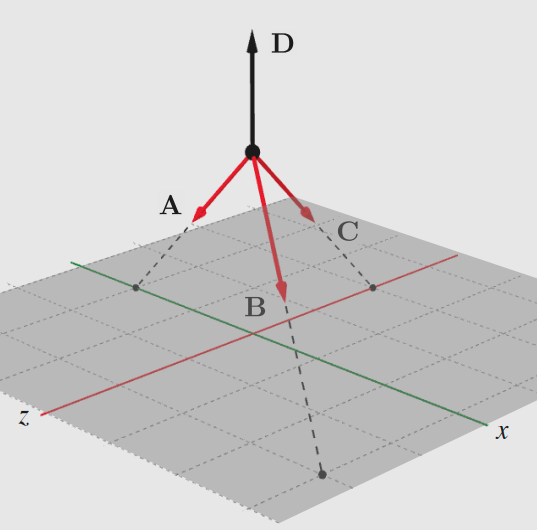
\includegraphics[width=\linewidth]{images/staticsballoon.png}
\label{fig:staticsballoon}
\end{wrapfigure}
Ans: 
\begin{align*}
    |\vec{A}| &= 463.57 \\ 
    |\vec{B}| &= 402.04 \\ 
    |\vec{C}| &= 309.05 
\end{align*}
\\[400pt]
}
\subsubsection{Qn: Engineering Statics Example 3.5.4 (Skycam)}
A skycam with weight of $\vec{W}$ is supported by tension in 3 cables $\vec{A}, \vec{B}, \vec{C}$ as shown in Figure \ref{fig:staticsskycam}. Given that the mass of the skycam is $20\text{ kg}$, what is the magnitude of the tension in each of the 3 cables? \\
\begin{wrapfigure}{r}{0.6\textwidth} 
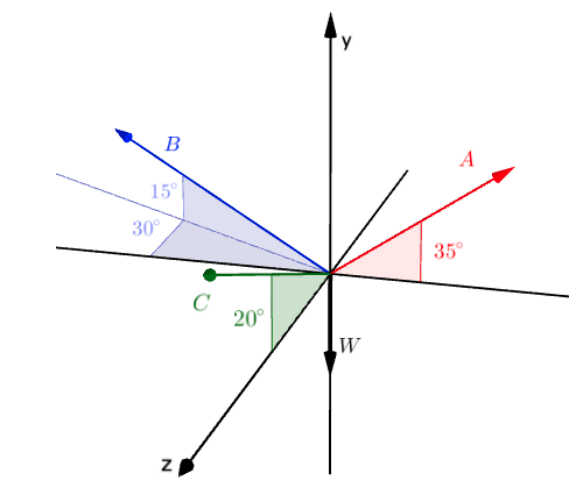
\includegraphics[width=\linewidth]{images/staticsskycam.png}
\label{fig:staticsskycam}
\end{wrapfigure}
Ans: \begin{align*}
    |\vec{A}| &= 196.4 \text{ N} \\ 
    |\vec{B}| &= 192.2 \text{ N} \\ 
    |\vec{C}| &= 98.5 \text{ N} 
\end{align*}
\clearpage
\subsection{Balancing Torque}
In order for rotational static equilibrium, net torque needs to be zero. i.e. 
$$\sum_i \tau_{i,x} = \sum_i \tau_{i,y} = \sum_i \tau_{i,z} = 0$$
Note: In physics olympiad, usually it suffices to consider torque in 2D. \\[10pt]
Recall that torque is always defined \textbf{about an origin} (of your choice). Your choice of origin will make a big difference in your quality of life when solving statics questions.
\subsubsection{Example: Lever}

\clearpage 
\subsubsection{(JUICY) Example: Hinged Shelf}
A shelf of mass $m$ is attached to the wall with a hinge at $P$ such that it can rotate freely about $P$ but not translate. The right end is held up by a string with tension $T$ at angle $\theta$. \\[5pt] 
(a) By considering torque about $P$, express $T$ in terms of $m,g,\theta$ \\[5pt] 
(b) By considering torque about the center of mass and horizontal forces, express $F_{\text{carry}}$ and $N$ in terms of $T,\theta$. \\
\begin{wrapfigure}{r}{0.5\textwidth} 
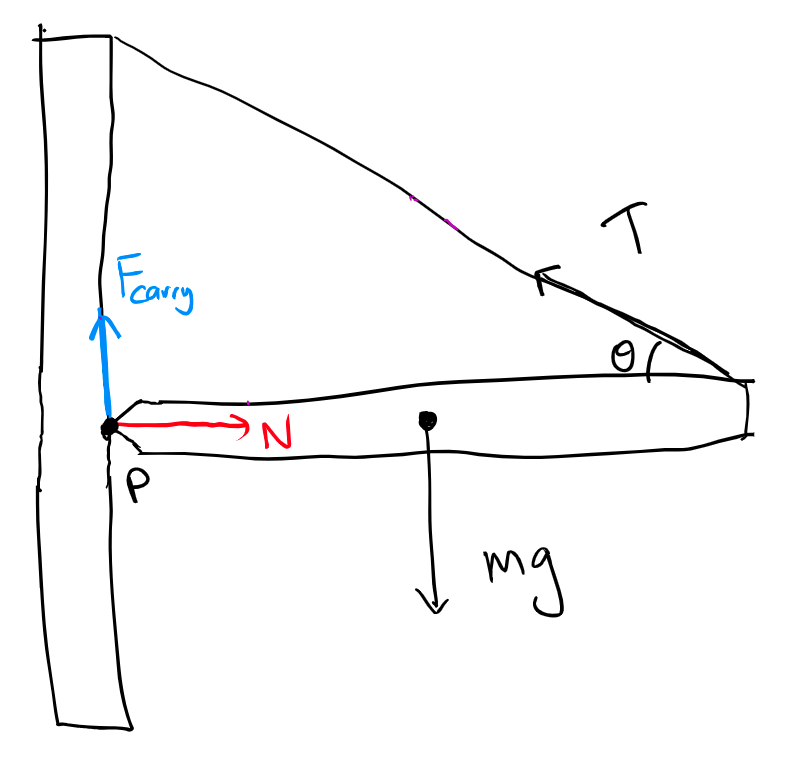
\includegraphics[width=\linewidth]{images/shelf0.png}
\label{fig:shelf}
\end{wrapfigure}
Ans: \\ (a) $T = \frac{mg}{2\sin\theta}$ \\ (b) $F_{\text{carry}} = T \sin \theta$, $N = T \cos \theta$\\[20pt]
Comment: This question teaches you that you can "eliminate" certain terms in your equation by choosing your axis to calculate torque wisely. Imagine if you knew $T$ but didn't know $mg$, or you knew $mg$ but didn't know $T$. Using this trick saves time and cuts down the algebra.
\clearpage
\subsection{3 Concurrent Forces: Intersection of 3 Lines}
\textbf{Theorem}: If an object is in static equilibrium (rotational and translational), and there are \textbf{only 3 forces} acting on it, then the 3 forces are concurrent (intersect at the same point).\\[10pt]
\textbf{Proof}: Consider the intersection $C$ of any 2 out of the 3 forces. By considering torque about $C$, the 2 forces exert no torque. To be in static equilibrium (no net torque), the 3rd force must also exert no torque. By line of action, the 3rd force must be concurrent (intersect at the same point).
\subsubsection{(JUICY) Example: Hinged Shelf (cont'd)}
A shelf of mass $m$ is attached to the wall with a hinge at $P$ such that it can rotate freely about $P$ but not translate. The right end is held up by a string with tension $T$ at angle $\theta$. \\[5pt]
(c) Find $|F_{\text{carry}}|/|N|$ in terms of $\theta$. \\[5pt] 
{
\begin{wrapfigure}{r}{0.5\textwidth} 
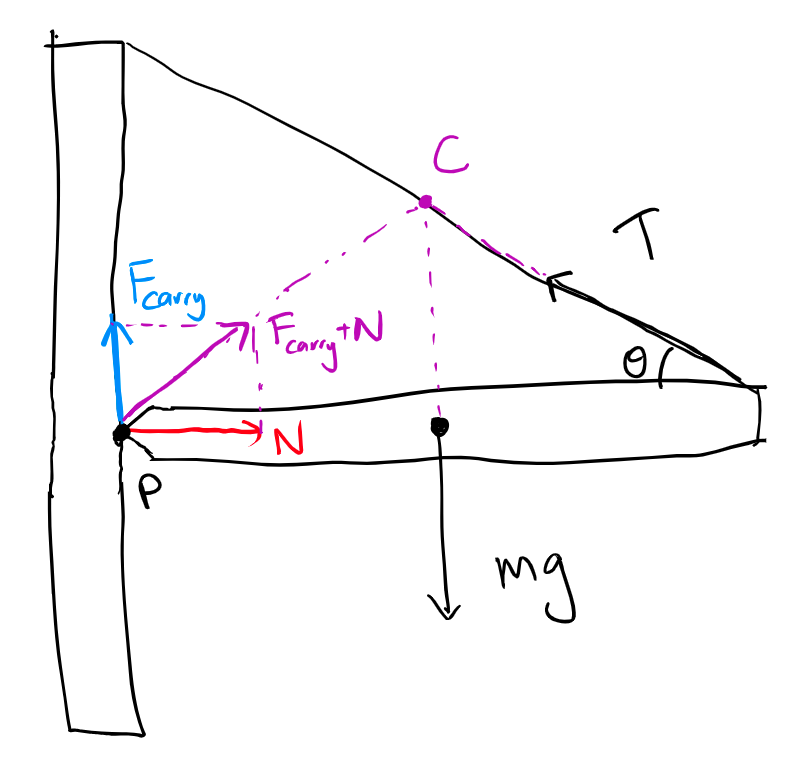
\includegraphics[width=\linewidth]{images/shelf.png}
\label{fig:shelf}
\end{wrapfigure}
Ans: $|F_{\text{carry}}|/|N| = \tan \theta$\\[200pt]
}
\clearpage

\subsubsection{(JUICY) Example: Morin Chap 2.2 (Leaning ladder)}
A ladder leans against a frictionless wall. If the coefficient of friction with the ground is $\mu$, what is the smallest angle the ladder can make with the ground and not slip?\\
\begin{wrapfigure}{r}{0.5\textwidth} 
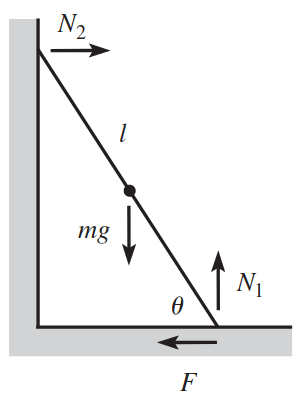
\includegraphics[width=\linewidth]{images/morinleaningladder.png}
\label{fig:morinleaningladder}
\end{wrapfigure}
Ans: $\tan \theta \leq \frac{1}{2\mu}$
\clearpage 
\section{Physics: Electrostatics (Point Charges)}
Every object has some amount of charge. "Electro" refers to the interaction of charges, "statics" mean that we are dealing with situations where the objects are not moving (in contrast with "dynamics"). In this section, we will talk about point charges, which are 0-dimensional objects that are precisely located at one point in space. This is an idealisation, and in the real world point charges don't exist. However, in most scenarios, one can prove that this idealisation will be "good enough", such the results we get from assuming our charges are point-like objects will coincide with the results we get if we had relaxed the assumption. Wherever applicable, we like to assume point charges because it makes the math easier.
\subsection{Electric Force}
If 2 point charges $Q$ and $q$ are separated by distance $r$, they exert (equal and opposite) forces on each other with magnitude 
\begin{align}
    | \vec{F}_{\text{Q on q}} | = | \vec{F}_{\text{q on Q}} | = \frac{k\ |Q|\ |q|}{r^2}
\end{align}
where $k = \frac{1}{4\pi\epsilon_0}$ is called Coulomb's constant. $\epsilon_0 = 8.85\times 10^{-12}\text{ Fm}^{-1}$ is the permittivity of vacuum. The unit F is Farad. \\[10pt]
The direction of the force depends on the relative sign of the 2 charges. If they are of the same sign (both positive or both negative), the direction of the force is radially outward (the force pushes the 2 charges away i.e. \textbf{like charges repel}). If they are of opposite sign (one negative and the other positive), the direction of the force is radially inward (the force pulls the 2 charges together i.e. \textbf{unlike charges attract}). We can summarise this in a single vector equation.
\begin{align}
    - \vec{F}_{\text{q on Q}} =\vec{F}_{\text{Q on q}} = \frac{kQq}{r^2} \hat{r} 
\end{align}
where $\hat{r}$ is the unit vector pointing from $Q$ to $q$.
\subsubsection{Principle of Superposition (Force)}
Note: The word superposition is used a lot all over physics to mean different things. It generally refers to the linearity of a system. \\[10pt]
If there are $N$ point charges $\{Q_1, Q_2, ..., Q_N\}$ (excluding our test charge), then the net force experienced by a test charge $q$ is just the sum of forces each charge individually exerts on it. 
\begin{align}
    \vec{F}_{\text{net on }q} = \sum_{i=1}^N \vec{F}_{Q_i \text{ on }q}
\end{align}
The proof of this is due to linearity of electric field (covered later). It is also verified experimentally.
\subsection{Electric Potential Energy (EPE)}
We won't be able to do the definition of EPE justice without mentioning line integrals, which we cover very soon. But for now, we take the following as fact. \\[10pt]
If 2 point charges $Q$ and $q$ are separated by distance $r$, the electric potential energy stored in this configuration is given by
\begin{align}
    U = \frac{kQq}{r}
\end{align}
Notice how EPE $U$ varies with respect to distance between the charges $r$.
\begin{itemize}
    \item For like charges ($Qq>0$), if the separation $r$ increases, the potential energy $U$ decreases.
    \item For unlike charges ($Qq<0$), if the separation $r$ increases, the potential energy $U$ increases.
\end{itemize}
Although we haven't talked about potential energy (and we can't until we talk about line integrals), there is a simple intuition I'd like to emphasise. \\[10pt]
Intuition: Nature generally seeks configurations that have \textbf{lower potential energy} (think of a ball on a hill). So for like charges, since potential energy decreases with increasing separation, \textbf{like charges naturally seek to increase their separation}, i.e. like charges repel. Likewise, for unlike charges, since potential energy decreases with decreasing separation, \textbf{unlike charges naturally seek to decrease their separation}, i.e. unlike charges attract.
\subsubsection{Principle of Superposition (EPE)}
The total potential energy of the system of $N$ charges $\{Q_1, Q_2, ..., Q_N\}$ is the \textbf{pairwise sum} of potential energies.
\begin{align}
    U_{\text{total}} = \sum_{1\leq i<j \leq N} U_{i,j} = \sum_{1\leq i<j \leq N} \frac{kQ_i Q_j}{r_{ij}}
\end{align}
This can be proved by constructing the configuration of charges one charge at a time. 
\subsection{Electric Field (from Electric Force)}
Note: At the moment, it seems almost redundant to define the electric field and potential. But from a theoretical point of view, the electric field and potential are actually more fundamental objects. The electric force and EPE are typically introduced first in most introductory courses/textbooks because they build on the student's pre-existing intuition for force and potential energy. The conceptual differences will become significant once we allow the charges to move, which we will study in Electrodynamics. \\[10pt]
A point charge has a charge $Q$ and is located at a point in space $\vec{r}_Q$ induces an electric field spanning all of space
\begin{align}
    \vec{E}(\vec{r}) = \frac{kQ}{|\vec{r} - \vec{r}_Q|^3} (\vec{r} - \vec{r}_Q)
\end{align}
I chose to put let the point charge be anywhere in space, but in most definitions you'll see the point charge placed at the origin $\vec{r}_Q = \vec{0}$, simplifying the electric field to
\begin{align}
    \vec{E}(\vec{r}) = \frac{kQ}{|\vec{r}|^2} \hat{r}
\end{align}
where $\hat r$ is a unit vector, pointing in the same direction as $\vec{r}$ but with length of 1. 
\subsubsection{Principle of Superposition (Field)}
If there are $N$ point charges $\{Q_1, Q_2, ..., Q_N\}$, then the electric field due to all these charges will be the \textbf{vector sum} of the electric field created by each individual charge. 
\begin{align}
    \vec{E}_{\text{total}}(\vec{r}) = \sum_{i=1}^N \vec{E}_{\text{due to }Q_i}(\vec{r})
\end{align}
This is due to linearity of Gauss' law (one of the 4 Maxwell equations). It is also verified experimentally.
\subsubsection{Force Per Unit Charge}
Electric Field is defined as the \textbf{force per unit charge} experienced by a \textbf{test charge}. In other words, if I put a test charge $q$ at a point $\vec{r}_q$, it would experience force 
\begin{align}
    \vec{F}_{\text{on }q} = q\vec{E}(\vec{r}_q)
\end{align}
It is often said that the test charge must be \textbf{infinitesimally small}, and the reason is that if it wasn't small, the test charge would exert a non-negligible force on the configuration of $N$ point charges, causing their positions to shift and changing the entire electric field. \\[10pt]
Even though the charge being infinitesimally small would result in the electric force on the test charge being infinitesimally small in magnitude as well, the ratio of $\vec{F} / q = \vec{E}$ will stay constant no matter how small $q$ is. This is akin to taking the derivative of a function $f'(x) = \lim_{h\rightarrow 0} [f(x+h)-f(x)]/h$ from first principles. 
\subsubsection{Cartesian Coordinates}
Lastly, I would like to write down the electric field in Cartesian coordinates and basis vectors, as an example of how to perform calculations using the above definition.
\begin{align}
    \vec{r} &= \left(\begin{array}{c}
         x \\
         y \\
         z 
    \end{array}\right) \\
    \hat{r} &= \frac{\vec{r}}{|\vec{r}|} = \frac{1}{\sqrt{x^2 + y^2 + z^2}} \left(\begin{array}{c}
         x \\
         y \\
         z 
    \end{array}\right)\\
    \vec{E}(x,y,z) &= \frac{kQ}{x^2 + y^2 + z^2} \frac{1}{\sqrt{x^2 + y^2 + z^2}} \left(\begin{array}{c}
         x \\
         y \\
         z 
    \end{array}\right) \\
    &= \frac{kQ}{(x^2 + y^2 + z^2)^{3/2}} \left(\begin{array}{c}
         x \\
         y \\
         z 
    \end{array}\right) 
\end{align}
\subsection{Electric Potential (from EPE)}
Similar to the electric field, the existence of an electric charge with charge $Q$ at position $\vec{r}_Q$ will cause an electric potential to permeate all of space
\begin{align}
    \phi(\vec{r}) = \frac{kQ}{|\vec{r} - \vec{r}_Q|}
\end{align}
Note: The electric potential $\phi(\vec{r})$ is a scalar field, as opposed to the electric field which is a vector field.\\[10pt]
And if $\vec{r}_Q = \vec{0}$ then
\begin{align}
    \phi(\vec{r}) = \frac{kQ}{|\vec{r}|}
\end{align}
\subsubsection{Potential Energy Per Unit Charge}
Similarly to the electric field, the electric potential is the potential energy per unit charge. If I put a test charge $q$ at position $\vec{r}_q$, the \textbf{increase} in potential energy of the configuration of charges will be
\begin{align}
    U_{\text{increase due to }q} = q\phi(\vec{r}_q) 
\end{align}
If the test charge $q$ is now added permanently to the configuration, then the electric potential will include it's contribution too (according to superposition principle).
\subsubsection{Principle of Superposition (Potential)}
The total electric potential due to a collection of $N$ charges $\{Q_1, Q_2, ..., Q_N\}$ will be the sum of the potentials due to each individual charge
\begin{align}
    \phi_{\text{total}}(\vec{r}) = \sum_{i=1}^N \phi_{\text{due to }Q_i}(\vec{r}) 
\end{align}
\subsubsection{Cartesian Coordinates}
Once again, I think it would be pedagogical if I write it out in Cartesian coordinates
\begin{align}
    \vec{r} &= \left(\begin{array}{c}
         x \\
         y \\
         z 
    \end{array}\right) \\
    \phi(\vec{r}) &= \frac{kQ}{\sqrt{x^2 + y^2 + z^2}}
\end{align}
\subsection{Exercises}
\subsubsection{SJPO 2016 General Round Q33}
4 point charges are arranged at the corners of a square of side length $\mathrm{d}$. The charges are as indicated on the diagram. What is the electric potential $V$ and the magnitude of the electrostatic force $F$ felt by a point charge of -1 e placed at the centre of the square? \\[0pt]
\begin{wrapfigure}{r}{0.4\textwidth} 
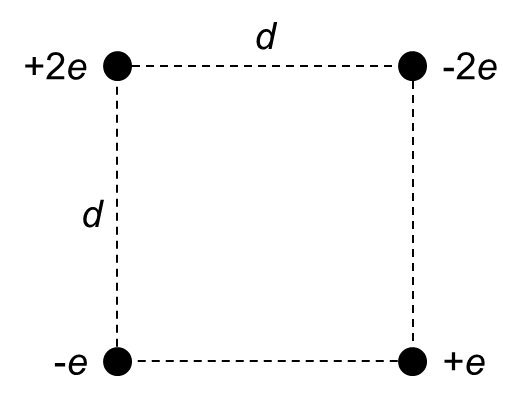
\includegraphics[width=\linewidth]{images/sjpo2016q33.png}
\end{wrapfigure}
\begin{itemize}
\item[] (A) $\quad V=0, F=\frac{1}{\sqrt{2}}\left(\frac{e^2}{\pi \varepsilon_0 d^2}\right)$
\item[] (B) $\quad V=0, F=\frac{e^2}{\pi \varepsilon_0 d^2}$
\item[] (C) $\quad V=0, F=0$
\item[] (D) $\quad V=\frac{1}{\sqrt{2}}\left(\frac{e}{\pi \varepsilon_0 d}\right), F=0$
\item[] (E) $\quad V=\frac{1}{\sqrt{2}}\left(\frac{e}{\pi \varepsilon_0 d}\right), F=\frac{1}{\sqrt{2}}\left(\frac{e^2}{\pi \varepsilon_0 d^2}\right)$
\end{itemize}
Ans: \ifpaper A \fi
\clearpage
\section{Math: Integration Techniques}
We introduce examples by techniques first. At the end we will summarise the different examples by their occurrence in physics, highlighting their similarities.
\subsection{Just Memorise}
For some integrals you just have to memorise the trick. For example
\begin{align}
    \int \sec x\ dx &= \ln |\sec x + \tan x| + C \\
    \int \sec^2 x\ dx &= \tan x + C 
\end{align}
\subsection{Integration by Parts}
If we consider the product rule
\begin{align}
    \frac{d}{dx} (UV) = \frac{dU}{dx} V + U \frac{dV}{dx}
\end{align}
Integrating both sides wrt $dx$ from $x=a$ to $x=b$, and rearranging,
\begin{align}
    \int_a^b U d V&=[U V]_a^b-\int_a^b V d U \\
    \int_a^b g \ f dx &= \left[ g\left(\int f dx \right) \right]_a^b - \int_a^b \left[ \left(\int f dx \right) \frac{dg}{dx}\right] dx 
\end{align}
My mnemonic is "integrate, keep, minus, integral of, integrate differentiate".\\[10pt]
You can use the following 2 expressions to remember integral by parts. The former one being a definite integral, the latter being an indefinite integral. Do note that in both expressions, $\displaystyle \left( \int f\ dx \right)$ does \textbf{not} include $+C$.
\begin{align}
    \int_a^b f g \ dx &= \Biggl[ \underbrace{\left(\int f\ dx \right)}_{\text{integrate}} \underbrace{\biggl. g \biggr.}_{\text{keep}} \Biggr]_a^b - \underbrace{\int_a^b dx }_{\text{integral of}}\Biggl[ \underbrace{\left(\int f\ dx \right)}_{\text{integrate}} \underbrace{\biggl.\frac{dg}{dx}\biggr.}_{\text{differentiate}}\Biggr] \\
    \int f g \ dx &= \Biggl[ \underbrace{\left(\int f\ dx \right)}_{\text{integrate}} \underbrace{\biggl. g \biggr.}_{\text{keep}} \Biggr] - \underbrace{\int dx }_{\text{integral of}}\Biggl[ \underbrace{\left(\int f\ dx \right)}_{\text{integrate}} \underbrace{\biggl.\frac{dg}{dx}\biggr.}_{\text{differentiate}}\Biggr] + C
\end{align}
It is best to just do a few exercises to find your \textbf{personal mnenomic} and stick to it.
\subsubsection{Exercises}
Show the following
\begin{align}
    \int \ln x \ dx &= x \ln x - x + C \\
    \int x \ln x \ dx &= \frac{x^2}{2} \ln x - \frac{x^2}{4} + C
\end{align}
\subsubsection{Physics Examples}

The following requires you to integrate by part twice and rearrange. \\
\noindent Source: \url{https://youtu.be/DoK5ZSGJNwE?t=485}
\begin{align}
    \text{Show that }\int_0^{\frac{\pi}{2}} T_0 e^{\mu \theta}(\mu \sin \theta+\cos \theta) d \theta = T_0 e^{\mu \frac{\pi}{2}}
\end{align}
\subsection{U-Substitution}
\subsubsection{$1/r$ integrals (potentials)}
\label{sec:potential_integral}
\begin{align}
& \int_{-b}^b \frac{d x}{\sqrt{x^2+a^2}} \\
& \text{Sub } x=a \tan \theta, \quad d x=a \sec ^2 \theta\ d \theta 
\end{align}
\begin{align}
\int_{\theta=\tan ^{-1}\left(-\frac{b}{a}\right)}^{\theta=\tan ^{-1}\left(\frac{b}{a}\right)} \frac{a \sec ^2 \theta\ d \theta}{\sqrt{a^2 \tan ^2 \theta+a^2}} &= \int_{-\tan ^{-1}\left(\frac{b}{a}\right)}^{\tan ^{-1}\left(\frac{b}{a}\right)}|\sec \theta|\ d \theta \\ 
& =\int_{-\alpha}^\alpha \sec \theta\ d \theta \text{    where } \alpha := \tan^{-1}(b/a) \notag \\
&= \ln \left| \frac{\sec \alpha + \tan \alpha}{\sec \alpha - \tan \alpha}\right| \\
&= \ln \left| \frac{\sec \left(\tan^{-1}(b/a)\right) + \tan \left(\tan^{-1}(b/a)\right)}{\sec \left(\tan^{-1}(b/a)\right) - \tan \left(\tan^{-1}(b/a)\right)}\right| \notag \\
&= \ln \left| \frac{\sqrt{1+\left(\frac{b}{a}\right)^2} + \frac{b}{a}}{\sqrt{1+\left(\frac{b}{a}\right)^2} - \frac{b}{a}}\right| \notag \\
&= 2 \ln \left( \sqrt{1+\left(\frac{b}{a}\right)^2} + \frac{b}{a} \right)
\end{align}
\subsubsection{$1/r^2$ integrals}
\begin{align}
& \int_{-b}^b \frac{d x}{{x^2+a^2}} \\
& \text{Sub } x=a \tan \theta, \quad d x=a \sec ^2 \theta\ d \theta 
\end{align}
\begin{align}
\int_{\theta=\tan ^{-1}\left(-\frac{b}{a}\right)}^{\theta=\tan ^{-1}\left(\frac{b}{a}\right)} \frac{a \sec ^2 \theta\ d \theta}{{a^2 \tan ^2 \theta+a^2}} &= \frac{1}{a} \int_{-\tan ^{-1}\left(\frac{b}{a}\right)}^{\tan ^{-1}\left(\frac{b}{a}\right)}\ d \theta \\ 
& = \frac{2}{a} \tan^{-1}\left(\frac{b}{a}\right)
\end{align}
\subsubsection{$1/r^3$ integrals (fields)}
\begin{align}
& \int_{-b}^b \frac{d x}{\sqrt{x^2+a^2}^3 } \\
& \text{Sub } x=a \tan \theta, \quad d x=a \sec ^2 \theta\ d \theta 
\end{align}
\begin{align}
\int_{\theta=\tan ^{-1}\left(-\frac{b}{a}\right)}^{\theta=\tan ^{-1}\left(\frac{b}{a}\right)} \frac{a \sec ^2 \theta\ d \theta}{\sqrt{a^2 \tan ^2 \theta+a^2}^3 } &= \frac{1}{a^2}\int_{-\tan ^{-1}\left(\frac{b}{a}\right)}^{\tan ^{-1}\left(\frac{b}{a}\right)} \cos \theta \ d \theta \\ 
& =\frac{1}{a^2} \int_{-\alpha}^\alpha \cos \theta\ d \theta \\
&= \frac{2}{a^2} \sin \alpha \\
&= \frac{2}{a^2} \sin \left( \tan^{-1} \left( \frac{b}{a} \right) \right)\\
&= \frac{2}{a^2} \frac{b}{\sqrt{a^2 + b^2}} 
\end{align}
\clearpage
\subsubsection{Geometrical Interpretation}
Draw a picture in lesson for the limits of integration.
\begin{figure}[h]
    \centering
    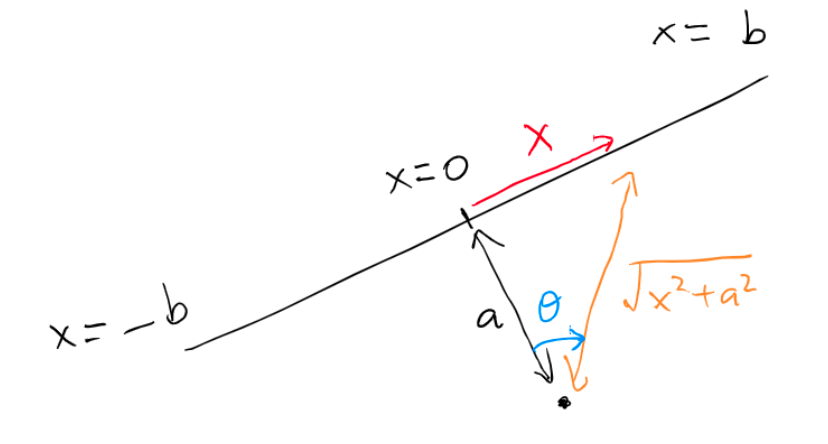
\includegraphics[width=0.5\linewidth]{images/usubgeom.png}
    \caption{U-substitution is a reparametrization of curve}
    \label{fig:usubgoem}
\end{figure}
\begin{figure}[h]
    \centering
    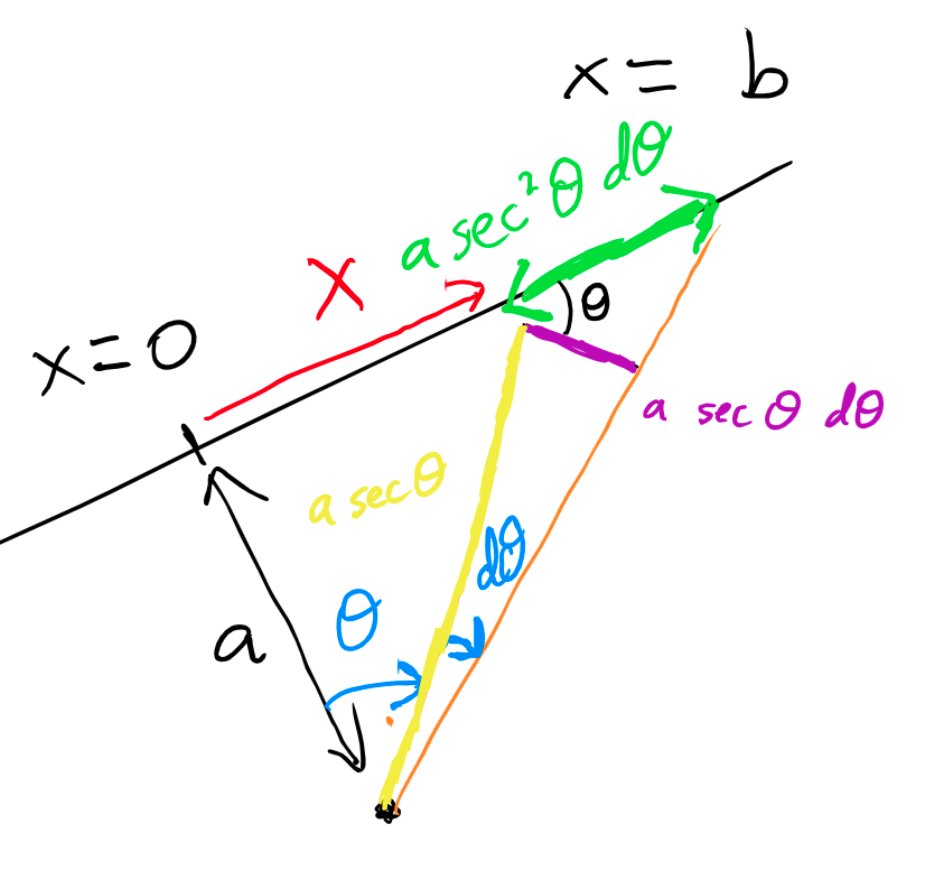
\includegraphics[width=0.5\linewidth]{images/usubgeom2.png}
    \caption{$dx=a \sec^2 \theta\ d\theta$ in greater detail}
    \label{fig:usubgeom2}
\end{figure}
% \subsection{Misc.}
\clearpage 
\section{Math: Line Integrals}
Let's begin by first mentioning a few examples of line integrals. 
\begin{align}
    \text{Work Done} &= \int_\gamma \vec{F}(\mathbf{s}) \cdot \overrightarrow{d\mathbf{s}} \\
    \phi(\rho) &= \int_\gamma \frac{k\ dq}{r} \\
    \vec{E}(\rho) &= \int_\gamma \frac{k \ dq}{r^2} \hat{r}
\end{align}
The common thing all these share is they are integrals over some curve $\gamma$. Pictorially (draw in class), 
\begin{figure}[h]
    \centering
    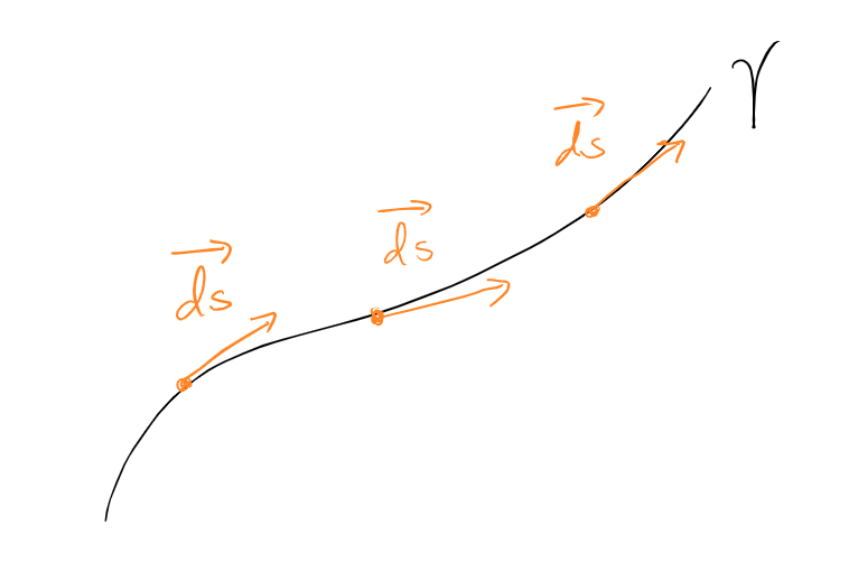
\includegraphics[width=0.5\linewidth]{images/lineintegral.png}
    \caption{$\overrightarrow{ds}$ is tangent vector to the curve}
    \label{fig:lineintegral}
\end{figure}\\
\subsection{Parametrization}
How do we actually perform such a calculation? We perform the following steps 
\begin{enumerate}
    \item Choose a parametrization of the curve $\gamma$
    $$\mathbf{s}(t) = \left(\begin{array}{l}
         x(t) \\
         y(t) \\
         z(t) 
    \end{array}\right) \stackrel{\text{e.g.}}{=} \left(\begin{array}{c}
         5 \sin 2t\\ t^2\\ -t
    \end{array}\right) \quad \text{ for } t \in [0,1]$$
    \item Differentiate the coordinates with respect to the parameter.
    $$\frac{\overrightarrow{d\mathbf{s}}}{dt} = \frac{d}{dt} \left(\begin{array}{c}
         x(t) \\
         y(t) \\
         z(t) 
    \end{array}\right) = \left(\begin{array}{c}
         10 \cos 2t\\ 2t\\ -1
    \end{array}\right)$$
    \item Substitute back into the integral
    $$\int_\gamma \vec{F}(\mathbf{s}) \cdot \overrightarrow{d\mathbf{s}} = \int_0^1 \vec{F}(\mathbf{s}(t)) \cdot \frac{\overrightarrow{d\mathbf{s}}}{dt} dt = \int_0^1 \vec{F}(\mathbf{s}(t)) \cdot \left(\begin{array}{c}
         10 \cos 2t\\ 2t\\ -1
    \end{array}\right) dt$$
    \item Evaluate the 1D integral 
    \begin{align}
    \vec{F}(x,y,z) &\stackrel{\text{e.g.}}{=} \left(\begin{array}{c}
         0 \\ z \\ 0
    \end{array}\right) \\
    \int_0^1 \vec{F}(\mathbf{s}(t)) \cdot \frac{\overrightarrow{d\mathbf{s}}}{dt} dt &= \int_0^1 \left(\begin{array}{c}
         0 \\ -t \\ 0
    \end{array}\right) \cdot \left(\begin{array}{c}
         10 \cos 2t\\ 2t\\ -1
    \end{array}\right) dt = \left[-\frac{2}{3} t^3\right]^1_0 = -\frac{2}{3} \notag
    \end{align}
\end{enumerate}
I would like to place emphasis on this step
\begin{align}
    \int_\gamma \vec{F}(\mathbf{s}) \cdot \overrightarrow{d \mathbf{s}}=\int_0^1 \vec{F}(\mathbf{s}(t)) \cdot \frac{\overrightarrow{d \mathbf{s}}}{d t} d t \label{eq:param}
\end{align}
It is the step where we go from an abstract integral over a curve to an actual calculation which we extract a numerical value from. Moreover, our choice of parametrization will determine how easy our calculation is. \\[10pt]
When we did the integral 
\begin{align}
    \int_{-b}^b \frac{d x}{{\sqrt{x^2+a^2}}^3} = \frac{1}{a^2} \left[ \frac{x}{\sqrt{x^2+a^2}} \right]^b_{-b} 
\end{align}
One can verify that the derivative of the RHS is indeed our integrand. However, it's not immediately obvious how one can go from the LHS to the RHS. In other words, if we had parametrized our curve using $x$, it is hard to perform the integral. However, choosing a different parametrization $\theta = \tan^{-1}(x/a)$ will make our life a lot easier
\begin{align}
    \int_{\theta=\tan ^{-1}\left(-\frac{b}{a}\right)}^{\theta=\tan ^{-1}\left(\frac{b}{a}\right)} \frac{a \sec ^2 \theta d \theta}{{\sqrt{a^2 \tan ^2 \theta+a^2}}^3}=\frac{1}{a^2} \int_{-\tan ^{-1}\left(\frac{b}{a}\right)}^{\tan ^{-1}\left(\frac{b}{a}\right)} \cos \theta d \theta
\end{align}
This is what we are actually doing when we do U-substitution. \\[10pt] \textbf{U-substitution is just a reparametrization of our curve!}\\[10pt]
Although it is easier to perform the calculation in the $\theta$ parametrization, it's geometrically easier to formulate the integral in the $x$ parametrization. U-substitution helps us reap the best of both worlds, by letting us formulate the geometry of the line integral in the $x$ parametrization, and evaluate the integral analytically using the $\theta$ parametrization in a systematic and purely algebraic way (so we won't need to think of the geometry). 
\subsection{Integrating Infinitesimal Charge $dq$}
One might see the line integral for electric potential \begin{align}
    \phi(\rho)=\int_\gamma \frac{k\ d q}{r}
\end{align}
and wonder where our familiar $\overrightarrow{d\mathbf{s}}$ went. In the context of physics, the curve $\gamma$ represents our line charge. Imagine a rope in 3D space, and imagine we sprinkle charges along the rope such that the rope now has charge distribution $\lambda(x)$. $dq$ means a "small segment of line charge" along our curve. If we parametrize our curve with parameter $x$, we may write $dq = \lambda(x)\ dx$. We will cover the example of "finite line charge" in greater detail later, but the parametrized integral will end up being 
\begin{align}
    \phi(\rho)=\int_\gamma \frac{k\ d q}{r} = \int_{-a}^a \frac{k \lambda(x)\ dx}{\sqrt{x^2 + \rho^2}}
\end{align}
\subsection{Integrating Vector Functions}
When we see a vector quantity in the integrand, such as in 
\begin{align}
    \vec{E}(\rho) &= \int_\gamma \frac{k \ dq}{r^2} \hat{r}
\end{align}
It just means we sum up vectors instead of scalars (real numbers). Numerically, it effectively means we perform 3 integrals instead of 1. In most physics questions, however, some components turn out to be zero by symmetry considerations (integral of an odd function vanishes). \\[10pt]
Also it's worth mentioning that when summing up vectors, our choice of coordinate system, and consequently the basis vectors, will determine the difficulty of the calculation. A common choice is the cylindrical coordinate basis vectors $\{\hat{\rho}, \hat{z}, \hat{\phi} \}$.

\section{Math: Cylindrical Coordinates Calculus}
\subsection{Recap: Polar Coordinates}
Refer to section \ref{sec:polar}.
\subsection{Cylindrical Coordinates}
The 3rd dimension is simply $\hat{z}$. Points in 3D space are labelled by coordinates $\rho, z, \phi$. \\[10pt]
\subsection{Cylindrical Basis Vectors}
Recall in section \ref{sec:polarbasis} that a basis vector \textbf{at a point P} is defined by "change \textbf{each} coordinate of P and see where it moves". With this, the basis vectors $\{\hat{rho}, \hat{z}, \hat{\phi}\}$ look like
\begin{figure}[h]
    \centering
    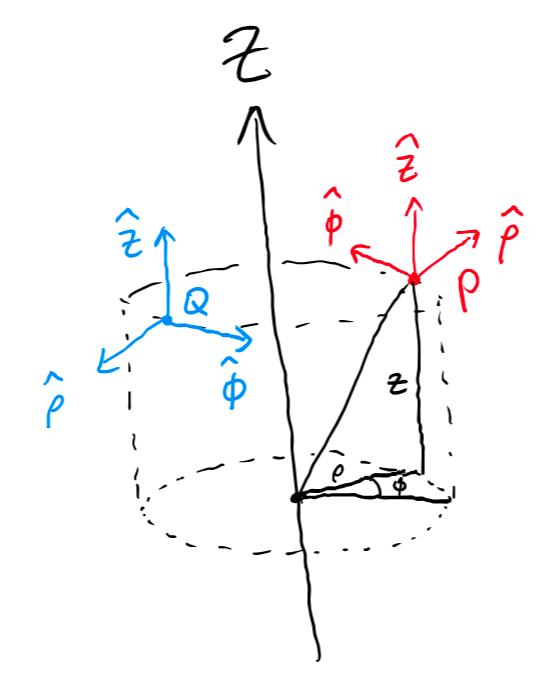
\includegraphics[width=0.5\linewidth]{images/cylindricalbasis2.png}
    \caption{Basis Vectors in Cylindrical Coordinates}
    \label{fig:cylindricalbasis}
\end{figure}\\[10pt]
The position vector is 
\begin{align}
    \vec{r} = \rho \hat{\rho} + z \hat{z}
\end{align}
We can differentiate this vector to obtain velocity and acceleration. We will end up with something like the centrifugal, Coriolis, and Euler force for the $\rho, \phi$ coordinates. This is because ${d\hat{\rho}}/{dt}$ involves both $\hat{\rho}$ and $\hat{\phi}$, and similarly for ${d\hat{\rho}}/{dt}$, whereas $d\hat{z}/dt$ is just $\dot{z} \hat{z}$. And $\hat{\rho}, \hat{\phi}$ change depending on where we are in space, while $\hat{z}$ is a constant basis vector everywhere.
\subsection{Integration in Cylindrical Coordinates}
One can see a nice table at \url{https://en.wikipedia.org/wiki/Del_in_cylindrical_and_spherical_coordinates}.
\subsubsection{Line Integral}
This is useful for Biot-Savart.
\begin{align}
{d\mathbf{s}} = d \rho\ \hat{{\rho}}+\rho\ d \phi \ \hat{{\phi}}+d z\ \hat{{z}}
\end{align}
How one can use the above, is by choosing a parameterization $t$ of the curve $\gamma$. Then recalling Equation \ref{eq:param}
\begin{align}
    \int_\gamma \mathbf{F}(\mathbf{s}) \cdot {d \mathbf{s}}=\int_0^1 \mathbf{F}(\mathbf{s}(t)) \cdot \frac{{d \mathbf{s}}}{d t} d t
\end{align}
Writing $\displaystyle \frac{d\mathbf{s}}{dt}$ from the RHS in polar coordinates means 
\begin{align}
{d\mathbf{s}} &= d \rho\ \hat{{\rho}}+\rho\ d \phi \ \hat{{\phi}}+d z\ \hat{{z}} \\ 
 &\  \bigg| \text{ "Divide" both sides by }dt\\
    \frac{d\mathbf{s}}{dt} &= \frac{d\rho}{dt} \hat{\rho} + \rho \frac{d\phi}{dt} \hat{\phi} + \frac{dz}{dt} \hat{z}
\end{align}
Note: Maybe you're confused about what $d\mathbf{s}$ is, it seems to be both an infinitesimal (due to the $d$) and a vector (due to bolded $\mathbf{s}$), or an "infinitesimal line segment". Moreover, you might be unsure what $d\rho$ on the RHS is (it's actually a "differential form"). \\[10pt]
\textbf{To resolve these conceptual confusions, choose a parameterization}, which means symbolically dividing it by $dt$. Then, it's now much clearer that $\displaystyle \frac{d\mathbf{s}}{dt}$ is the vector tangent to the curve, and $\displaystyle \frac{d\rho}{dt}$ is the derivative of the curve's $\rho(t)$ coordinate with respect to time.\\[10pt]
Extra: In most cases, the value of the line integral \textbf{depends on the path/curve taken}, which means that to calculate the result, we definitely have to parameterize it. However, in some special cases known as \textbf{conservative vector fields}, one can show that the result is independent of our path. In such cases, the vector field $\mathbf{F}(\mathbf{s})$ can be written directly in terms of $\rho, \phi, z$ and their respective basis vectors (e.g. $\mathbf{F} = (1/\rho) \hat{\rho}$ for infinite line charge), and so we can evaluate the line integral without choosing any parameterization. We will talk about conservative vector fields in the Vector Calculus chapter.
\subsubsection{Surface Integral}
This probably isn't used much.
\begin{align}
{d\mathbf{A}} = \rho\ d \phi\ d z\ \hat{{\rho}} 
+d \rho\ d z\ \hat{{\phi}}
+\rho\ d \rho\ d \phi\ \hat{{z}}
\end{align}
We will talk about surface integrals in detail later.
\subsubsection{Volume Integral}
This is useful in Moment of Inertia calculations.
\begin{align}
dV = \rho\ d \rho\ d \varphi\ d z
\end{align}
We will talk about volume integrals in detail later.

\section{Physics: Electrostatics (1D Examples)}
We consider charges of the following shapes
\begin{itemize}
    \item Ring Charge
    \item Finite Line 
    \item Infinite Line 
    % \item Square Loop 
\end{itemize}

\subsection{Ring Charge (Axial)}
"Axial" means along the axis perpendicular to the plane spanned by the ring charge.
\begin{figure}[h]
    \centering
    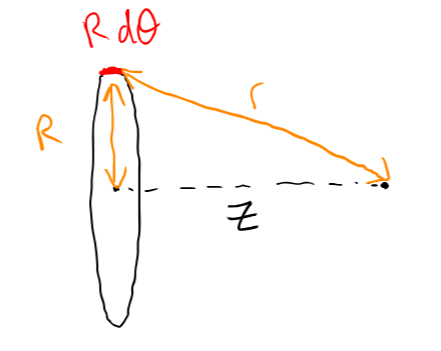
\includegraphics[width=0.8\linewidth]{images/ringcharge.png}
    \caption{Ring Charge}
    \label{fig:ringcharge}
\end{figure}\\[10pt]
We can parameterize the ring by an angle $\theta$, then the infinitesimal charge $ds = R\ d\theta$ where $R$ is the radius of the ring. $dq = k \lambda\ ds = k \lambda R\ d\theta$ and $r = \sqrt{z^2 + R^2}$. \\[10pt]
Calculating the potential,
\begin{align}
\phi(z) &= \int_\mathcal{C} \frac{k\ dq}{r} \\ 
&=\int_0^{2 \pi} \frac{k \lambda R\ d \theta}{\sqrt{z^2+R^2}} \\
&= \frac{ \lambda R}{2 \epsilon_0 \sqrt{z^2+R^2}} 
\end{align}
where we substituted $k=1/4\pi\epsilon_0$ in the final expression. \\[10pt]
For the electric field,
\begin{align} 
\vec{r}&=z \hat{z}-R \hat{\rho} \\
d \vec{E}&= \frac{k\ dq}{r^3} \vec{r}\\
&=\frac{k \lambda R\ d \theta}{\sqrt{z^2+R^2}^3}(z \hat{z}-R \hat{\rho}) \\
&= \frac{k \lambda R\ d \theta}{\sqrt{z^2+R^2}^3}z\ \hat{z}- \frac{k \lambda R\ d \theta}{\sqrt{z^2+R^2}^3} R\ \hat{\rho} \\
&= dE_z\ \hat{z} + dE_\rho\ \hat{\rho} \\
E_\rho &= 0 \text{ by symmetry} \\
E_z&=\int_0^{2 \pi} \frac{k \lambda R\ d \theta}{{\sqrt{z^2+R^2}}^3} z \\
&= \frac{ \lambda R z}{{2\epsilon_0 \sqrt{z^2+R^2}}^3} 
\end{align}
Once again, you can verify that $E_z = -\frac{\partial \phi}{\partial z}$.

\subsection{Finite Line Charge}
Suppose we have a straight line charge of length $2a$ and charge density $\rho$. Find the potential $\phi(\rho)$ and electric field $\vec{E}(\rho)$ at distance $\rho$ away from the center of the line charge.
\begin{figure}[h]
    \centering
    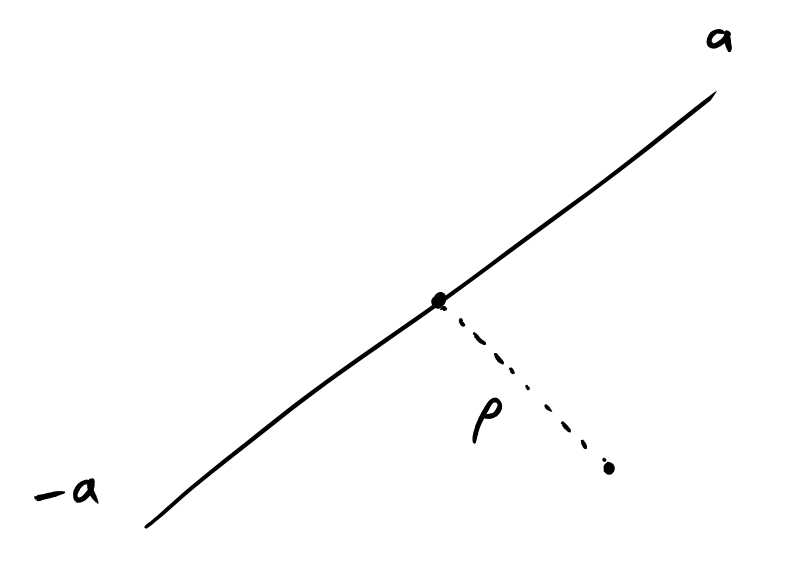
\includegraphics[width=0.8\linewidth]{images/finiteline.png}
    \caption{Finite Line Charge}
    \label{fig:finiteline}
\end{figure}
\subsubsection{Potential}
Each small charge $dq$ contributes $\displaystyle d\phi = \frac{k\ dq}{r}$ to the potential, where $r$ is the distance from the infinitesimal charge $dq$ to the point in space where we are measuring the potential of. Pictorially
\begin{figure}[h]
    \centering
    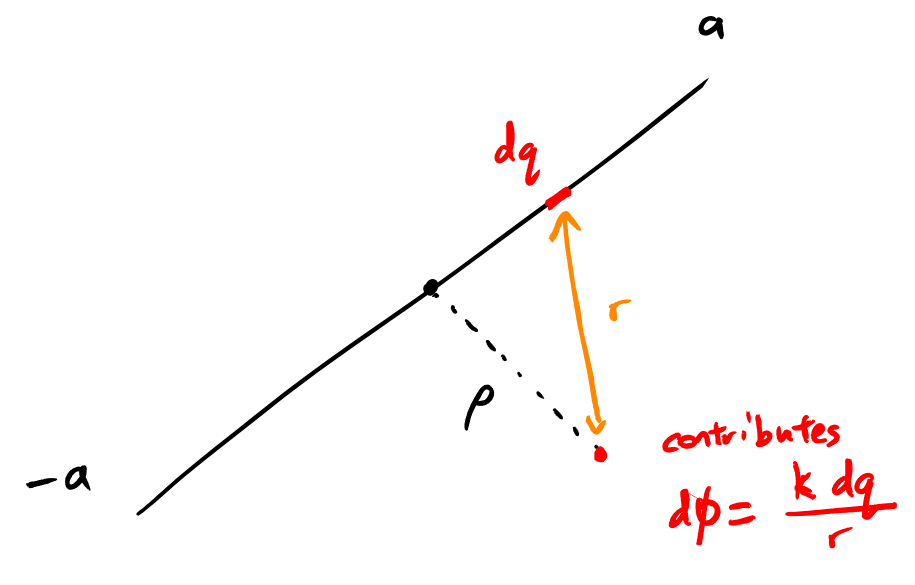
\includegraphics[width=0.8\linewidth]{images/finiteline2.png}
    \caption{Each $dq$ contributes $d\phi$}
    \label{fig:finiteline2}
\end{figure}\\[10pt]
The total electric potential will hence be 
\begin{align}
    \phi(\rho)=\int_\gamma \frac{k\ d q}{r}
\end{align}
where $\gamma$ is the curve representing the line charge. To evaluate this line integral, we choose a parameterization for the curve. In this case we choose $z$ as the parameter.
\begin{align}
    \phi(\rho)&=\int_{-a}^a \frac{k \lambda\ d z}{\sqrt{z^2+\rho^2}} 
\end{align}
This is just the integral in Section \ref{sec:potential_integral}. Evaluating it yields 
\begin{align}
    \phi(\rho) &= 2k\lambda \ln \left( \sqrt{1+\left(\frac{a}{\rho}\right)^2} + \frac{a}{\rho}\right)
\end{align}
Right now we see that if we take the limit $\lim_{a\rightarrow\infty}$, the potential at a finite distance will diverge $\phi(\rho) \rightarrow \infty$. One also observes that the answer is only dependent on the ratio $a/\rho$.
\subsubsection{Electric Field}
Now let's turn out attention to calculating the Electric Field. We will be integrating the the infinitesimal Electric Field (a vector)
\begin{align}
    d\vec{E} &= \frac{k \lambda d z}{{\sqrt{z^2+\rho^2}}^3} \vec{r} \\
    \text{where }\vec{r} &= -z \hat{z} + \rho \hat{\rho} 
\end{align}
Because the direction of $\vec{r}$ changes depending on where you are along the $z$-axis, we need to decompose $\vec{r}$ into \textbf{constant bases} before we perform integration
\begin{align}
\text{Substituting } \vec{r} &= -z \hat{z} + \rho \hat{\rho} \\
    d\vec{E} &= \frac{-z k \lambda d z}{{\sqrt{z^2+\rho^2}}^3} \hat{z}+\frac{\rho k \lambda d z}{{\sqrt{z^2+\rho^2}}^3} \hat{\rho} \\ 
    &= dE_z\ \hat{z} + dE_{\rho}\ \hat{\rho} 
\end{align}
Integrating $dE_z$ and $dE_\rho$ we obtain
\begin{align}
    E_z &= \int_{-a}^{a} \frac{-z k \lambda d z}{{\sqrt{z^2+\rho^2}}^3} = 0 \\
    E_\rho &= \int_{-a}^{a} \frac{\rho k \lambda d z}{{\sqrt{z^2+\rho^2}}^3} = 2k\lambda \frac{  a}{\rho \sqrt{a^2 + \rho^2}}
\end{align}
where $E_z=0$ follows from the fact that the integrand is an odd function.\\[10pt]
Extra: One can verify that electric field is the gradient of potential $$E_\rho = -\frac{\partial \phi(\rho)}{\partial \rho}$$

\subsection{Infinite Line Charge}
\subsubsection{Electric Field}
Taking the limit $a\rightarrow\infty$, we get
\begin{align}
    \lim_{a\rightarrow\infty} E_\rho&= 2 k \lambda\lim_{a\rightarrow\infty} \frac{a}{\rho \sqrt{a^2+\rho^2}} \\
    &=  2 k \lambda\lim_{a\rightarrow\infty} \frac{1}{\rho \sqrt{1+\left(\frac{\rho}{a}\right)^2}}\\
    &= \frac{2k\lambda}{\rho}
\end{align}
\subsubsection{Potential (First Attempt: Pesky Infinity)}
One can take the limit $a\rightarrow\infty$. One sees that 
\begin{align}
    \lim_{a\rightarrow\infty}\phi(\rho)&=2 k \lambda  \lim_{a\rightarrow\infty}\ln \left(\sqrt{1+\left(\frac{a}{\rho}\right)^2}+\frac{a}{\rho}\right) = \infty 
\end{align}
This may seem unintuitive as the potential is infinity no matter where we are in space, but yet there is a notion of "location A has higher potential than location B" which leads to the non-zero electric field. The correct intuition is that wherever you are, you experience electric field proportional to $1/\rho$, which causes you to accelerate and gain kinetic energy by Work-Energy theorem. Suppose you place a stationary test charge at location X with the same polarity as the infinite line charge. As it get repelled, the amount of kinetic energy it gains is proportional to $1/\rho$, which means it approaches $0$ as you move to infinity. However, even though the contribution converges to zero, the partial sum of contributions diverges (\href{https://en.wikipedia.org/wiki/Harmonic_series_(mathematics)}{Harmonic Series}). As it flies off to infinity, it gains infinite amount of kinetic energy. This implies that the potential at the starting location X is infinity. \\[10pt]
The same argument can be made for a test charge of opposite polarity, except it flies towards the line charge instead.
\subsubsection{Potential}
There is a way to resolve the issue of $\phi(\rho) = \infty$ so that we get $\phi(\rho) = - 2k \lambda \ln \rho$, which matches textbook results. Resolving this will also be a pedagogical exercise in solidifying our conceptual understanding. \\[10pt]
\textbf{Point}: Only potential \textit{differences} matter.\\[10pt]
The electric potential difference between two points is defined by 
\begin{align}
    \phi_{B} - \phi_{A} = -\int_A^B \vec{E} \cdot d\vec{s}
\end{align}
For the infinite line charge, 
\begin{align}
    \vec{E} = \frac{2k\lambda}{\rho}\ \hat{\rho} 
\end{align}
(Extra: Because this vector field is curl-free, line integral doesn't depend on path taken)\\[10pt]
Choosing a radial path from $A$ to $B$, we get
\begin{align}
    \phi_B - \phi_A &= -\int_A^B \vec{E} \cdot d\vec{s} \\
    &= -\int_{\rho_A}^{\rho_B} \frac{2k\lambda}{\rho} d\rho \\
    &= - 2k\lambda \ln \left( \frac{\rho_B}{\rho_A} \right) \\ 
    &= - 2k\lambda \left( \ln \rho_B - \ln \rho_A \right) 
\end{align}
Or for an indefinite integral,
\begin{align}
    \phi(\rho) &= -2k \lambda \ln \rho + C \\
    \text{where } C &\text{ is an arbitrary constant}
\end{align}
Even though this \textit{seems like} doesn't make sense dimensionally since we can't plug in a dimensional quantity $\rho$ (meters) into the $\ln$ function, the $C$ here actually saves the day. $C/2k\lambda$ has units of $\ln (\text{meters})$, and if we write $C = 2k\lambda \ln \rho_0$ then $C$ sets the radius $\rho_0$ of \textit{zero potential}.
\begin{align}
    \phi(\rho) = -2k \lambda \ln \left(\frac{\rho}{\rho_0}\right) \label{eq:phirho}
\end{align}
We could choose any distance $\rho_0$ to be our point of zero potential. \\[10pt]
Remark: In fact, this illuminates why our first attempt gets infinity for the potential! When we said that each infinitesimal line element $dq$ had potential of $d\phi = k\ dq / r$, we implicitly set the zero potential to be at infinity. That worked well for the point charge, but if we set $\rho_0=\infty$ in \ref{eq:phirho}, we see that gives us $\phi(\rho) = -2k \lambda \ln 0 = \infty$. \\[10pt]
\textbf{When} we set the location of zero potential matters! The 2 attempts of calculating potential of line charge
\begin{enumerate}
    \item E field of point charge $\Rightarrow$ Potential of point charge $\Rightarrow$ Potential field of line charge
    \item E field of point charge $\Rightarrow$ E field of line charge $\Rightarrow$ Potential of line charge
\end{enumerate}
Calculation 1 yields infinity because when we go from E field to potential (of point charge), we implicitly set the point of zero potential to be at infinity. \\[10pt]
Calculation 2 yields a sensible potential function because when we go from E field to potential (of line charge), we set the point of zero potential to be some finite distance.
\section{Math: Spherical Coordinates Calculus}
\section{Math: 2D Integrals}
\section{Physics: Electrostatics (2D Examples)}
\begin{itemize}
    \item Infinite Sheet 
    \item Spherical Shell (Inside)
    \item Spherical Shell (Outside)
    \item Disk (Axial) (Morin)
    \item Disk (Rim) (Morin)
\end{itemize}
\section{Math: Surface Integrals}
\subsection{Moment of Inertia}
Integrating scalar functions over a surface is something we need to perform, for say, finding the moment of inertia of a 2D laminar. Once again, to calculate a surface integral, we need to find a parameterization of the surface. We illustrate this with the following examples:
\begin{itemize}
    \item Rectangular Laminar
    \item Disk (Perpendicular Axis)
    \item Disk (Parallel Axis)
\end{itemize}
\subsubsection{Rectangular Laminar}
We may parameterize a rectangular surface $\mathcal{S}$ as 
\begin{align}
\mathcal{S} = \{(x,y)\ \vert -a/2 \leq x \leq a/2,\ -b/2 \leq y \leq b/2 \}
\end{align}
Then performing the integral would just be substituting the parameterization into the limits of integration
\begin{align}
    I &= \iint_{\mathcal{S}} r^2\ dm \\
    &= \int_{y=-b/2}^{y=b/2} \underbrace{\int_{x=-a/2}^{x=a/2} (x^2 + y^2)\ \sigma dx}dy \\
    &= \sigma \int_{y=-b/2}^{y=b/2} \left[ \frac{x^3}{3} + xy^2 \right]^{x=a/2}_{x=-a/2} \ dy \\
    &= \sigma \int_{y=-b/2}^{y=b/2} \left( \frac{a^3}{12} + ay^2 \right)  \ dy\\
    &= \sigma \left[ \frac{a^3}{12}y + \frac{ay^3}{3} \right]^{y=b/2}_{y=-b/2} \\ 
    &= \sigma \left(\frac{a^3 b}{12} + \frac{a b^3}{12} \right) \\
    &= \frac{1}{12} m (a^2 + b^2)
\end{align}
\subsubsection{Disk (Perpendicular Axis)}
Parameterizing the disk $\mathcal{S}$ as 
\begin{align}
    \mathcal{S} = \{ (\rho,\theta)\ \vert\ 0 \leq \rho \leq R, \ 0 \leq \theta \leq 2\pi \} 
\end{align}
And remembering that for polar coordinates, the differential area form 
\begin{align}
    dA = \rho\ d\rho \ d\theta
\end{align}
Finding the moment of inertia of the disk about an axis perpendicular to the disk,
\begin{align}
    I &= \iint_\mathcal{S} r^2\ dm \\
    &= \int_{\theta=0}^{\theta=2\pi} \int_{\rho=0}^{\rho=R} \rho^2\ \sigma \ \rho\  d\rho \ d\theta \\
    &= \sigma \int_{\theta=0}^{\theta=2\pi} \left[\frac{\rho^4}{4}\right]^R_0 d\theta \\
    &= \frac{m}{\pi R^2} \int_{\theta=0}^{\theta=2\pi} \left(\frac{R^4}{4}\right) d\theta \\
    &= \frac{m}{\pi R^2} 2\pi \frac{R^4}{4} \\
    &= \frac{1}{2} m R^2
\end{align}
\subsubsection{Disk (Parallel Axis)}
We parameterize the disk the same way, except now the distance $r$ to the parallel axis is
\begin{align}
    r = \rho \sin \theta
\end{align}
So the moment of inertia with respect to an axis parallel to the disk is
\begin{align}
    I &= \iint_\mathcal{S} r^2\ dm \\
    &= \int_{\theta=0}^{\theta=2\pi} \int_{\rho=0}^{\rho=R} \rho^2 \sin^2 \theta \ \sigma \ \rho\  d\rho \ d\theta \\
    &= \sigma \int_{\theta=0}^{\theta=2\pi} \left[\frac{\rho^4}{4}\right]^R_0 \sin^2 \theta\ d\theta \\
    &= \frac{m}{\pi R^2} \int_{\theta=0}^{\theta=2\pi} \left(\frac{R^4}{4} \sin^2 \theta \right) d\theta \\
    &= \frac{m}{\pi R^2} \frac{R^4}{4} \pi \\
    &= \frac{1}{4} m R^2
\end{align}
\subsection{Flux}
Flux of a vector field $\vec{E}$ through a surface $\mathcal{S}$ is given by 
\begin{align}
    \Phi = \iint_\mathcal{S} \vec{E} \cdot \overrightarrow{dA}
\end{align}
We need to parameterize the surface as usual, but this time our $\overrightarrow{dA}$ is a vector. The simplest example would be a point charge and a spherical surface surrounding it.
\subsubsection{Point Charge}
To calculate the electric flux of a point charge, through a spherical Gaussian surface $\mathcal{S}$ centered at the point charge, we can parameterize the Gaussian surface as
\begin{align}
    \mathcal{S} &= \{ (\rho,\theta,\varphi)\ \vert\ \rho = R,\ \theta \in [0,\pi],\ \varphi \in [0,2\pi] \} \\
    \overrightarrow{dA} &= \rho^2 \sin \theta\ d\theta\ d\varphi\ \hat{\rho} + \rho\sin\theta\ d\rho\ d\varphi\ \hat{\theta} + \rho\ d\rho\ d\theta\ \hat{\varphi} 
\end{align}
where we obtained $\overrightarrow{dA}$ from \url{https://en.wikipedia.org/wiki/Del_in_cylindrical_and_spherical_coordinates}. \\[10pt]
The electric field of a point charge is 
\begin{align}
    \vec{E} = \frac{kQ}{\rho^2} \hat{\rho}
\end{align}
Hence the flux may be evaluated
\begin{align}
    \Phi &= \iint_\mathcal{S} \vec{E} \cdot \overrightarrow{dA} \\
    &= \iint_\mathcal{S} \frac{kQ}{\rho^2} \hat{\rho} \cdot (\rho^2 \sin \theta\ d\theta\ d\varphi\ \hat{\rho} + \rho\sin\theta\ d\rho\ d\varphi\ \hat{\theta} + \rho\ d\rho\ d\theta\ \hat{\varphi}) \\
    &= \iint_\mathcal{S} \frac{kQ}{\rho^2} \hat{\rho} \cdot \rho^2 \sin \theta\ d\theta\ d\varphi\ \hat{\rho} \\
    &= \int_0^{\pi} d\theta \int_0^{2\pi} d\varphi \frac{kQ}{\rho^2} \rho^2 \sin \theta \\
    &= kQ \int_0^{\pi} d\theta \int_0^{2\pi} d\varphi \sin \theta \\
    &= 2\pi kQ \int_0^{\pi} d\theta\ \sin \theta \\
    &= 4\pi kQ \\
    &= \frac{Q}{\epsilon_0}
\end{align}
This is a boring result, but it does illustrate how one performs flux calculations. Another boring result you can check is that the flux of a dipole is $0$.
\subsubsection{Point Charge (Cartesian)}
We could very well have chosen a different parameterization of our Gaussian surface,
\begin{align}
    \mathcal{S} &= \{ (x,y,z)\ \vert\ x^2 + y^2 + z^2 = R \}  \\
    \overrightarrow{dA} &= dx\ dy\ \hat{z} + dy\ dz\ \hat{x} + dx\ dz\ \hat{y}
\end{align}
This leads to a more complicated integral where the symmetry of the problem is not manifest, but it'll be a good exercise to verify that it leads to the same answer for flux.
\section{Gauss Law \& Gaussian Surfaces}
The integral form of Gauss law for electric field is 
\begin{align}
    \iint_\mathcal{S} \mathbf{E} \cdot d\mathbf{A} = \frac{Q_{\text{enclosed}}}{\epsilon_0}
\end{align}
The integral form of Gauss law for magnetic field is 
\begin{align}
    \iint_\mathcal{S} \mathbf{B} \cdot d\mathbf{A} = 0
\end{align}
\subsection{Infinite Sheet revisited}
Consider a pillbox as a Gaussian surface. The flux through the sides of the pillbox are $0$ since the electric field is purely vertical due to symmetry of the system. Hence, the total flux is through the top and bottom surfaces of the cylindrical pillbox. By Gauss' law, 
\begin{align}
    \Phi_{\text{top}} + \Phi_{\text{bottom}} = \frac{\sigma A}{\epsilon_0}
\end{align}
Since $\Phi_{\text{top}} = \Phi_{\text{bottom}}$, 
\begin{align}
    \Phi_{\text{top}} = \frac{\sigma A}{2\epsilon_0}
\end{align}
The flux is also by definition 
\begin{align}
    \Phi_{\text{top}} = E_{z} A 
\end{align}
So equating the two gets us
\begin{align}
    E_{z} = \frac{\sigma}{2\epsilon_0}
\end{align}
which coincides with the answer we get through direct integration over the infinite surface.
\subsection{Shell Theorem}
\textbf{Theorem}: A spherically symmetric charge distribution affects \textbf{external} objects as though all the charge was concentrated at a point at its center.\\[10pt]
(Draw picture in class) Consider a spherical Gaussian surface of radius $R$ around the charge distribution. By spherical symmetry, total flux is just 
\begin{align}
    \Phi = E\ 4\pi R^2
\end{align}
Gauss Law tells us 
\begin{align}
    \Phi = \frac{Q}{\epsilon_0}
\end{align}
where $Q$ is the total charge of the charge distribution. Equating the two, the electric field is 
\begin{align}
    E = \frac{kQ}{R^2}
\end{align}
which is the same result if we pretended all the charge was concentrated into a point charge at the center of the charge distribution. \\[10pt]
\textbf{Note:} If you are inside the charge distribution, however, you need to be more careful when calculating how much charge your Gaussian surface encloses. Let's illustrate this with an example.
\subsection{Uniformly Charged Solid Sphere}
\textbf{Qn}: If we have a uniformly charged solid (not hollow) sphere of radius $R$ with charge density $\rho$, find the electric field $E$ and potential $\phi$ as a function of distance $r$ from the center. Consider regions both inside and outside the sphere. \\[10pt]
We first find the electric field using Gaussian surface, then we integrate it to find the potential. 
\subsection{Exercises}
(Competitive Physics 5.4.1) Problem: Determine the electric field at a point $\frac{l}{2}$ above the center of a square with a uniform surface charge density $\sigma$ and edge length $l$. \\[20pt]
Prove Earnshaw's theorem with Gauss' theorem.
\section{Math: 3D Integrals}
\section{Math: Volume Integrals}
\begin{itemize}
    \item Filled Shell (Inside/Outside)
\end{itemize}
\section{Assorted Questions II}
\subsubsection{SJPO 2016 General Round Q25}
A circular disc with an axle of diameter $2 \mathrm{~cm}$, is attached with strings to the ceiling. The disc is rotated so that the strings wind up along the axle so that the disc is raised up to the ceiling. The string is long such that that when the disc is released from rest, its center of mass falls $2.0 \mathrm{~m}$. The disc does not slip from the string. Assume that the axle is massless and the disc has all of its $5 \mathrm{~kg}$ mass at radius $3 \mathrm{~cm}$. Estimate the acceleration of the center of mass of the disc near the bottom of the fall. \\
{
\begin{wrapfigure}{r}{0.4\textwidth} 
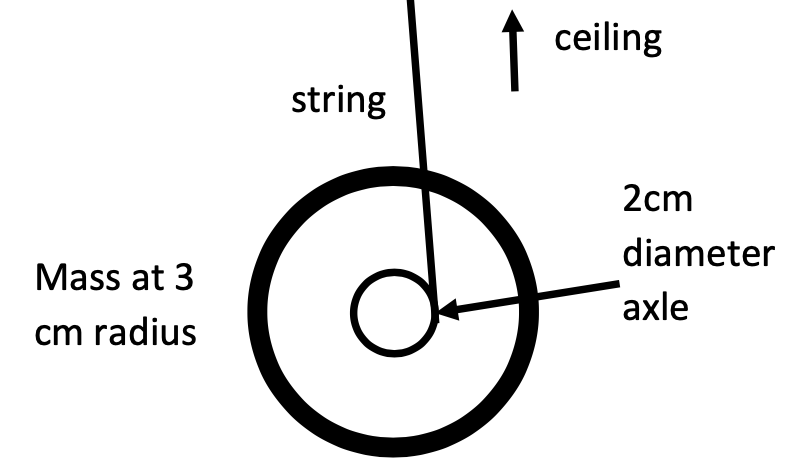
\includegraphics[width=\linewidth]{images/sjpo2016q25.png}
\end{wrapfigure}
\begin{itemize}
\item[](A) $g$
\item[](B) $2 g / 3$
\item[](C) $g / 3$
\item[](D) $g / 5$
\item[](E) $g / 10$
\end{itemize}
}
\subsubsection{SJPO 2018 General Round Q4}
A sphere rolls without slipping down a rough inclined plane. The gain in rotational kinetic energy is due directly to the work done by
\begin{itemize}
\item[](A) Static friction
\item[](B) Kinetic friction
\item[](C) Weight
\item[](D) Normal contact force
\item[](E) Air resistance
\end{itemize}
\subsubsection{Taylor Problem 3.5}
Consider an elastic collision between two \textbf{equal mass} bodies, one of which is initially at rest. Let their velocities be $\mathbf{v}_1$ and $\mathbf{v}_2=0$ before the collision, and $\mathbf{v}_1^{\prime}$ and $\mathbf{v}_2^{\prime}$ after. Show that $\mathbf{v}_1^{\prime} \cdot \mathbf{v}_2^{\prime}=0$. \\[10pt]
Extra: This result was important in the history of atomic and nuclear physics: That two bodies emerged from a collision traveling on perpendicular paths was strongly suggestive that they had equal mass and had undergone an elastic collision.
\subsubsection{(JUICY) Sliding Mass Down a Hemisphere}
A small marble placed at the top of a smooth hemisphere slides off the hemisphere. At what angle $\theta$ from the vertical does the marble lose contact with the hemisphere?
\subsubsection{Morin Problem 2.4 (Keeping a book up)}
A book of mass $M$ is positioned against a vertical wall. The coefficient of friction between the book and the wall is $\mu$. You wish to keep the book from falling by pushing on it with a force $F$ applied at an angle $\theta$ with respect to the horizontal $(-\pi / 2<\theta<\pi / 2)$, as shown in Figure \ref{fig:morinkeepingbookup}. \\[10pt]
{
(a) For a given $\theta$, what is the minimum $F$ required? \\[5pt]
(b) For what $\theta$ is this minimum $F$ the smallest? What is the corresponding minimum $F$ ?\\[5pt]
(c) What is the limiting value of $\theta$, below which there does not exist an $F$ that keeps the book up?\\[5pt]
\begin{wrapfigure}{r}{0.4\textwidth} 
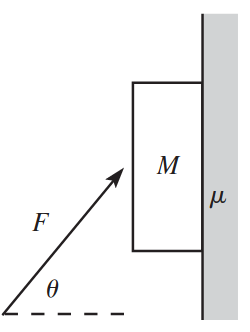
\includegraphics[width=\linewidth]{images/morinkeepingbookup.png}
\label{fig:morinkeepingbookup}
\end{wrapfigure}
}
\clearpage
\subsubsection{Morin Problem 2.14 (Leaning sticks)}
One stick leans on another as shown in Figure \ref{fig:morin2.14}. A right angle is formed where they meet, and the right stick makes an angle $\theta$ with the horizontal. The left stick extends infinitesimally beyond the end of the right stick. The coefficient of friction between the two sticks is $\mu$. The sticks have the same mass density per unit length and are both hinged at the ground. What is the minimum angle $\theta$ for which the sticks don't fall? \\
{
\begin{wrapfigure}{r}{0.4\textwidth} 
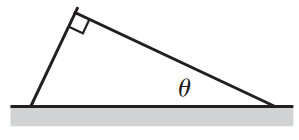
\includegraphics[width=\linewidth]{images/morin2.14.png}
\label{fig:morin2.14}
\end{wrapfigure}\\[70pt]
}
\subsubsection{Morin Problem 2.15 (Supporting a ladder)}
A ladder of length $L$ and mass $M$ has its bottom end attached to the ground by a pivot. It makes an angle $\theta$ with the horizontal and is held up by a massless stick of length $\ell$ that is also attached to the ground by a pivot (see Figure \ref{fig:morin2.15}). The ladder and the stick are perpendicular to each other. Find the force that the stick exerts on the ladder.\\
{
\begin{wrapfigure}{r}{0.4\textwidth} 
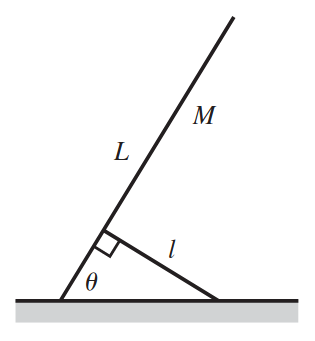
\includegraphics[width=\linewidth]{images/morin2.15.png}
\label{fig:morin2.15}
\end{wrapfigure}
}
\clearpage
\subsubsection{(JUICY) Morin Problem 7.8 (Wrapping around a pole)}
A puck of mass $m$ sliding on frictionless ice is attached by a horizontal string of length $\ell$ to a thin vertical pole of radius $R$. The puck initially travels in (essentially) a circle around the pole at speed $v_0$. The string wraps around the pole, and the puck gets drawn in and eventually hits the pole. What quantity is conserved during this motion? What is the puck's speed right before it hits the pole?\\[5pt]

\clearpage

\section{Physics: Springs}
\subsubsection{SJPO 2018 General Round Q19}
Two adventurous Physics students, each weighing $60 \mathrm{~kg}$, jump off a $43 \mathrm{~m}$ high bridge on a Bungee cord. The length of the cord is such that the students together will just touch the water and rebound. While Bungee cords become softer (more elastic) with increasing extension, for our calculations we can approximate the cord as having a constant stiffness of $k=330 \mathrm{~N} / \mathrm{m}$, and we can ignore the height of the students and where the cord is tied on their body. What is the unstretched length of the cord?
\begin{itemize}
\item[] (A) $10.0 \mathrm{~m}$
\item[] (B) $17.5 \mathrm{~m}$
\item[] (C) $25.5 \mathrm{~m}$
\item[] (D) $32.5 \mathrm{~m}$
\item[] (E) $40.0 \mathrm{~m}$
\end{itemize}
\subsubsection{SJPO 2016 General Round Q13}
An ideal uniform spring of mass $m \mathrm{~kg}$, unstretched length $L \mathrm{~m}$ and spring constant $k\  \mathrm{Nm}^{-1}$ stretches by an extension of $x \mathrm{~m}$ when hung vertically. Which statement below is correct? (You may want to know that the sum of $\mathrm{N}$ terms in an arithmetic progression from 1 to $\mathrm{N}$ is $\frac{N(N+1)}{2}$)
\begin{itemize}
\item[] (A) The top half of the spring with mass $\frac{m}{2} \mathrm{~kg}$ has an extension $\frac{x}{2} \mathrm{~m}$.
\item[] (B) The top half of the spring with length $\frac{L+x}{2} \mathrm{~m}$ supports $\frac{m g}{2} \mathrm{~N}$.
\item[] (C) The top half of the spring with mass $\frac{m}{2} \mathrm{~kg}$ has a spring constant of $\frac{k}{2} \mathrm{Nm}^{-1}$.
\item[] (D) The extension of the whole spring is $\frac{m g}{k} \mathrm{~m}$
\item[] (E) The length of the whole spring is $L+\frac{m g}{2 k} \mathrm{~m}$
\end{itemize}
Ans: \ifpaper E \fi

\clearpage
\section{Physics: Center of Mass}
\subsubsection{SJPO 2018 General Round Q5}
A thin wire is bent into the form of a three-sided shape as shown below. Each segment has equal length $l$. The height of the centre of mass from the bottom of the shape is \\
{
\begin{wrapfigure}{r}{0.3\textwidth}
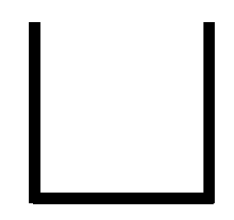
\includegraphics[width=1.0\linewidth]{images/sjpo2018q5.png}
\end{wrapfigure}
\begin{itemize}
\item[] (A) $l / 2$
\item[] (B) $2 l / 3$
\item[] (C) $l / 3$
\item[] (D) $l / 4$
\item[] (E) $2 l / 5$
\end{itemize}
}

\subsubsection{SJPO 2018 General Round Q20}
A dog weighing $10 \mathrm{~kg}$ is standing on a flatboat so that he is $20 \mathrm{~m}$ from the shore. The boat weighs $40 \mathrm{~kg}$ and has uniform mass distribution. The dog walks $8.0 \mathrm{~m}$ on the boat towards the shore and stops. For this calculation, one can assume no friction or drag between the boat and the water. How far is the dog from the shore now? \\
{
\begin{wrapfigure}{r}{0.6\textwidth}
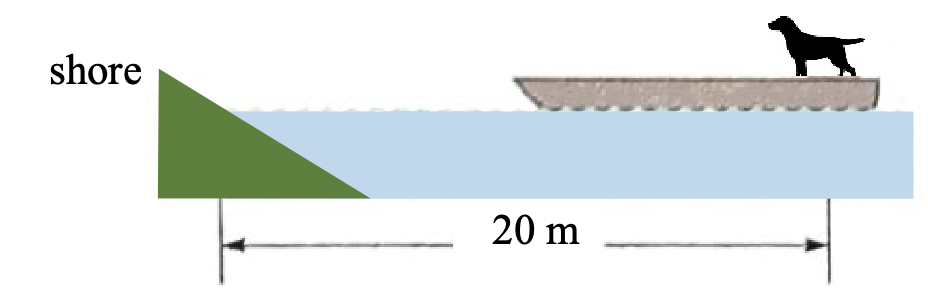
\includegraphics[width=1.0\linewidth]{images/sjpo2018q20.png}
\end{wrapfigure}
\begin{itemize}
\item[] (A) $12.0 \mathrm{~m}$
\item[] (B) $13.6 \mathrm{~m}$
\item[] (C) $14.0 \mathrm{~m}$
\item[] (D) $16.8 \mathrm{~m}$
\item[] (E) $29.8 \mathrm{~m}$
\end{itemize}
}
\clearpage


\section{Physics: Moment of Inertia}
Examples: uniform rod, uniform disc, shell, solid sphere, rectangular plate, griffiths textbook exercises.

\subsubsection{SPhO 2020 Q1}
A cylindrical rod has a radius of 1.0 cm and length 1.0 m. It is made up of two sections, each of length 0.5 m. The material of one section is zinc and that of the other section is copper. The end of the rod made of zinc is pivoted to a fixed point O. The rod is first held so that it is horizontal and then released. Determine the angular velocity of the rod when it is in the vertical position. (Densities: zinc: 7135 kg $\text{m}^{-3}$; copper: 8940 kg $\text{m}^{-3}$) [10]\\
\noindent Ans: $0.91258 \text{ kg m}^2$
\clearpage
\section{Math: Vector Calculus}
\noindent The approach I will take in this book will differ from conventional methods. I plan to use surface and line integrals to introduce divergence and curl respectively. 
\clearpage
\section{Physics: Potentials \& Potential Energy}
\subsubsection{SJPO 2018 General Round Q1}
The figure shows the potential energy $V(x)$ as a function of molecular separation $x$ for a diatomic molecule of reduced mass $\mu$.
If $V(x)=V_0\left(1-e^{-\left(x-x_0\right)/\delta}\right)^2-V_0$, the vibrational frequency $f$ at the equilibrium position is
(Hint: This series expansion may be useful. $e^x \approx 1+x+\frac{x^2}{2 !}$ ) \\
\begin{wrapfigure}{r}{0.6\textwidth}
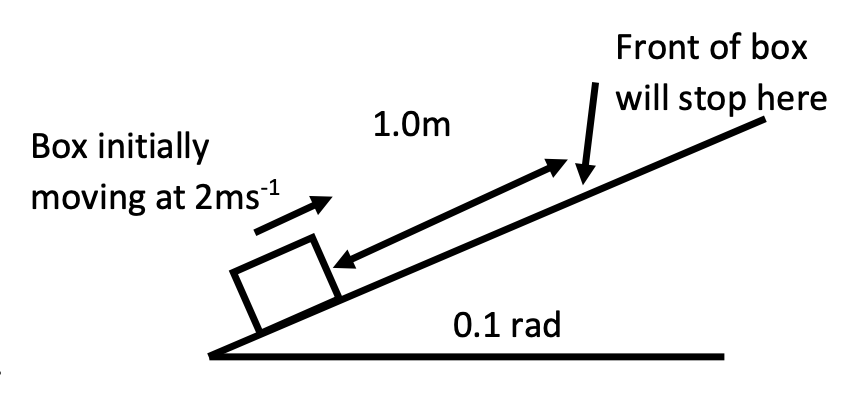
\includegraphics[width=1.0\linewidth]{images/sjpo2016q4.png}
\end{wrapfigure}
\begin{itemize}
\item[] (A) $\frac{2 V_0}{\mu \delta}$
\item[] (B) $\frac{V_0}{2 \pi^2 \mu \delta}$
\item[] (C) $\sqrt{\frac{2 V_0}{\mu \delta^2}}$
\item[] (D) $\frac{1}{2 \pi} \sqrt{\frac{2 V_0}{\mu \delta^2}}$
\item[] (E) $\frac{1}{2 \pi} \sqrt{\frac{V_0}{\mu \delta^2}}$
\end{itemize}
Ans: \ifpaper D \fi
\clearpage
\section{Physics: Electromagnetism}
\section{Physics: AC Circuits}

\section{Math: Differential Equations}
\subsection{SHM: Driven and Damping}
\subsection{Laplace Transform}

\section{Physics: Ropes}
\subsection{Friction - Capstan Equation}
\section{Physics: Pulleys}
\subsubsection{Qn: Morin Problem 8.1 (Massive pulley)}
Consider the Atwood's machine shown in Figure \ref{fig:morin8.1}. The masses are $m$ and $2 m$, and the pulley is a uniform disk of mass $m$ and radius $r$. The string is massless and does not slip with respect to the pulley. Find the acceleration of the masses. Use conservation of energy. \\
\begin{wrapfigure}{r}{0.6\textwidth}
\includegraphics[width=1.0\linewidth]{images/morin8.1.png}
\label{fig:morin8.1}
\end{wrapfigure}
Ans: $2g/7$
\section{Physics: DC Circuits}
\section{Physics: Effective Resistance}
\subsection{Equipotential Method}
\subsection{Recursive}
\subsubsection{SJPO 2014 General Round Q35}
As shown in the following figure, each resister has a resistance of $R$. What is the effective resistance between point $a$ and $b$ ?
\begin{wrapfigure}{r}{0.6\textwidth}
\includegraphics[width=1.0\linewidth]{images/sjpo2016q4.png}
\end{wrapfigure}
\begin{itemize}
\item[] (A) $(1+\sqrt{3}) R$
\item[] (B) $(1+\sqrt{5}) R$
\item[] (C) $(1+\sqrt{5}) R / 2$
\item[] (D) $(1+\sqrt{3}) R / 2$
\item[] (E) $R$
\end{itemize}
Ans: \ifpaper A \fi 
\subsection{Injecting Current}
\subsection{Extra: Circuit Laplacian}
\section{Physics: Fluid Mechanics}
\section{Physics: Waves}
\section{Physics: Optics}
\section{Physics: Thermodynamics}
\section{Physics: Non-Inertial Reference Frame}

\subsubsection{SJPO 2014 General Round Q34}
A candle is lighted in a gas jar as shown below. If the jar swings in a circle about O at a constant speed, in which direction will the flame of the candle point?
\begin{wrapfigure}{r}{0.6\textwidth}
\includegraphics[width=1.0\linewidth]{images/sjpo2014q34.png}
\end{wrapfigure}
\begin{itemize}
\item[] (A) Forward, in the direction of motion.
\item[] (B) Backward, opposite to its velocity.
\item[] (C) Still vertically upwards.
\item[] (D) Inward, points towards $\mathrm{O}$.
\item[] (E) Outwards, away from O.
\end{itemize}
Ans: \ifpaper D \fi

\subsubsection{SJPO 2018 General Round Q3}
A plumb line is held steady while being carried in a moving train. The mass of the plumb bob is $m$, and the train is accelerating in the forward direction at $0.5 g$. What is the tension in the string?
\begin{itemize}
\item[] (A) $0.5 mg$
\item[] (B) $1.12 mg$
\item[] (C) $1.22 mg$
\item[] (D) $2 mg$
\item[] (E) Cannot be determined from the given information.
\end{itemize}
\end{document}
